\clearpage
\chapter{HNL discovery with the DUNE experiment}
\label{cha:hnl_dune}

In a \emph{beam dump} experiment, an energetic beam of protons is directed into %
a fixed dense block of material, such as concrete or graphite, %
in order to absorb the hadronic cascade and stop secondary charged particles.
This facilitates the study of stable and long-lived particles.
The approach resembles accelerator neutrino experiments, in which %
the production of pions, kaon, and muons is maximised to generate an intense and focused neutrino beam.
A crucial difference between oscillation detectors and %
dedicated beam dump searches of the past is that the former are devised to enhance %
the SM neutrino scattering rate, while the latter try to suppress it in order to reduce %
backgrounds and favour the search for exotic and rare long-lived particles.
It is exciting to note, however, that neutrino oscillation detectors are able to %
perform beam-dump-like measurements~\cite{Kusenko:2004qc, Asaka:2012bb, Abe:2019kgx}. 
This is most favourable for searches of heavy neutral leptons (HNL), %
since they could be produced at accelerator facilities in the beam %
with light neutrinos (see \refsec{sec:production}).
The HNL can subsequently decay in one of the ways described in \refsec{sec:decay} inside a detector %
in proximity of the beam target, leaving a detectable signature.
The event rate is directly linked to the sterile--active neutrino mixings of the extended PMNS matrix.
The strongest limits on mixing angles with heavy states were set by %
the PS191 experiment~\cite{Bernardi:1985ny, Bernardi:1987ek}, a beam dump experiment which ran at CERN in 1984.
Its most stringent upper bounds on the novel mixing angles are $|U_{eN}|^2 \leq \np{e-8}$ and %
$|U_{\mu N}|^2 \leq \np{e-9}$ for neutrino masses between the pion and the kaon mass.
Powerful proton beams and strong particle reconstruction capabilities of current and upcoming %
neutrino detectors will allow competitive searches for heavy and long-lived neutrinos %
and possible improvement of present limits.
Among the running experiments, T2K has recently reached similar constraints to PS191~\cite{Abe:2019kgx}.
As an example of planned experiments, it has been shown that the Short Baseline Neutrino (SBN) program~\cite{Antonello:2015lea} %
can reach interesting bounds on HNL searches~\cite{Ballett:2016opr}, despite a naively large background  %
which can be controlled thanks to the distinctive kinematics of neutrino decays and %
the high performance of Liquid Argon (LAr) technologies.
Future long baseline oscillation experiments, such as the Deep Underground Neutrino Experiment %
(DUNE)~\cite{Abi:2018dnh}, will see a greatly diluted flux of nearly-sterile neutrinos %
at their far detectors and consequently poor sensitivity.
However, the near detector of DUNE (DUNE ND), placed \np{574}\,m from the target, has a great potential %
for searches for new physics~\cite{Adams:2013qkq}.
Close proximity to a very intense neutrino beam and cutting-edge event reconstruction capabilities %
will allow DUNE ND to undertake valuable searches for BSM physics in a entirely complementary way %
to the central oscillation physics programme. 

In this chapter, a detailed analysis of the sensitivity of DUNE ND to HNL in beam-dump-style searches is presented.
The following analysis is based on the theoretically consistent models from \refcha{cha:mass_models}, %
in which sterile neutrinos are associated with neutrino mass generation via a low-scale seesaw mechanism.
In particular, the production modes of \reftab{tab:branch} and most of the decay channels of \reftab{tab:decays} %
are considered.
The analysis presented here is refined and extended in comparison with previous works~\cite{Krasnov:2019kdc, Adams:2013qkq}, %
thanks to the polarised rates computed in \refcha{cha:mass_models} and the latest configuration of the DUNE ND~\cite{Abi:2020wmh}.
The ND and the neutrino beam are described in \refsec{sec:dunend}; %
a first estimate of the $\nu_\tau$ flux component is also presented.
The simulation used to compute the number of HNL decays at the ND site is explained in \refsec{sec:experiment}, %
and possible backgrounds for the most relevant discovery channels are there discussed.
Results of the sensitivity to HNL discovery are reported in \refsec{sec:results}.
Finally discussions of the possibility of resolving mass models and the fermionic nature of HNLs is %
carried out respectively in \refsec{sec:combined} and \refsec{sec:majorana_dirac}.

%Differently from previous sensitivity studies
%we ground our discussion in theoretically consistent models, in which sterile neutrinos are associated with neutrino %
%mass generation via a low-scale seesaw mechanism. %, such as inverse seesaw (ISS) mechanisms.
%We note that the range of masses and mixing angles testable at DUNE~ND is of interest for the generation of %
%the baryon asymmetry in the context of the ASR mechanism~\cite{Akhmedov:1998qx, Asaka:2005pn, Hernandez:2015wna, Hernandez:2016kel, Drewes:2017zyw}.
%We consider both Majorana and pseudo-Dirac states and calculate their decay and production rates, 
%with careful consideration given to helicity arguments.
%These formulae are then used to estimate the sensitivity of the experiment, %
%taking into account the beam and detector performance capabilities thanks to simulations of both event and background signals.
%We stress that DUNE will be able to extend the current limits on new fermionic singlets, %
%including those with masses above 500\,MeV, probing models of theoretical significance for the generation of neutrino mass.
%We show that bounds can be put also on the mixing with tau neutrinos, thanks to the high energy~beam.

\section{The near detector of DUNE}
\label{sec:dunend}

DUNE~\cite{Abi:2018dnh} is a long-baseline oscillation experiment that %
will study neutrino physics in great detail, focusing mainly on the determination %
of the CP violating phase, $\delta_\text{CP}$, and the mass ordering, i.e.\ the sign of $\Delta m_{32}^2$, %
and on the precision measurement of other oscillation parameters, in particular $\theta_{23}$.
These goals can be achieved thanks to both an intense neutrino beam and a high-resolution Far Detector (FD), %
consisting of a 40\,kt Liquid Argon Time Projection Chamber (LArTPC), situated \np{1300}\,km from the beam target.
The drift velocity of ionised electrons in LAr, typically of the order of cm/\textmu s, %
can be controlled with sufficient precision, by tuning the electric field, %
to result in high spatial resolution for event reconstruction~\cite{Rubbia:1977zz}.
The LAr is advantageous compared to the gaseous counterpart because it is around one thousand times denser, %
increasing the interaction probability, which is valuable for neutrino physics.
Employing very pure argon, the recombination of released electrons can be reduced and %
so the LArTPC design can be scaled to large volumes, as it will be done for DUNE.
To overcome high-purity challenges, the TPC can be operated in dual phase mode, in which a portion of the chamber is filled %
with argon vapour.
Once the drifting electrons are extracted from the liquid phase to the gaseous one, %
avalanche multiplication of the electrons amplifies the signal.
LAr also scintillates with a high light yield, around 40 photons/keV and differently from other %
liquefied noble gasses LAr is transparent to its scintillation wavelength, which peaks at \np{126.8}~nm.
A photo-detection system can collect the scintillation light giving an additional handle on event reconstruction.
All these exceptional properties make LArTPC a powerful tool for precision neutrino physics.

\begin{figure}
	\centering
	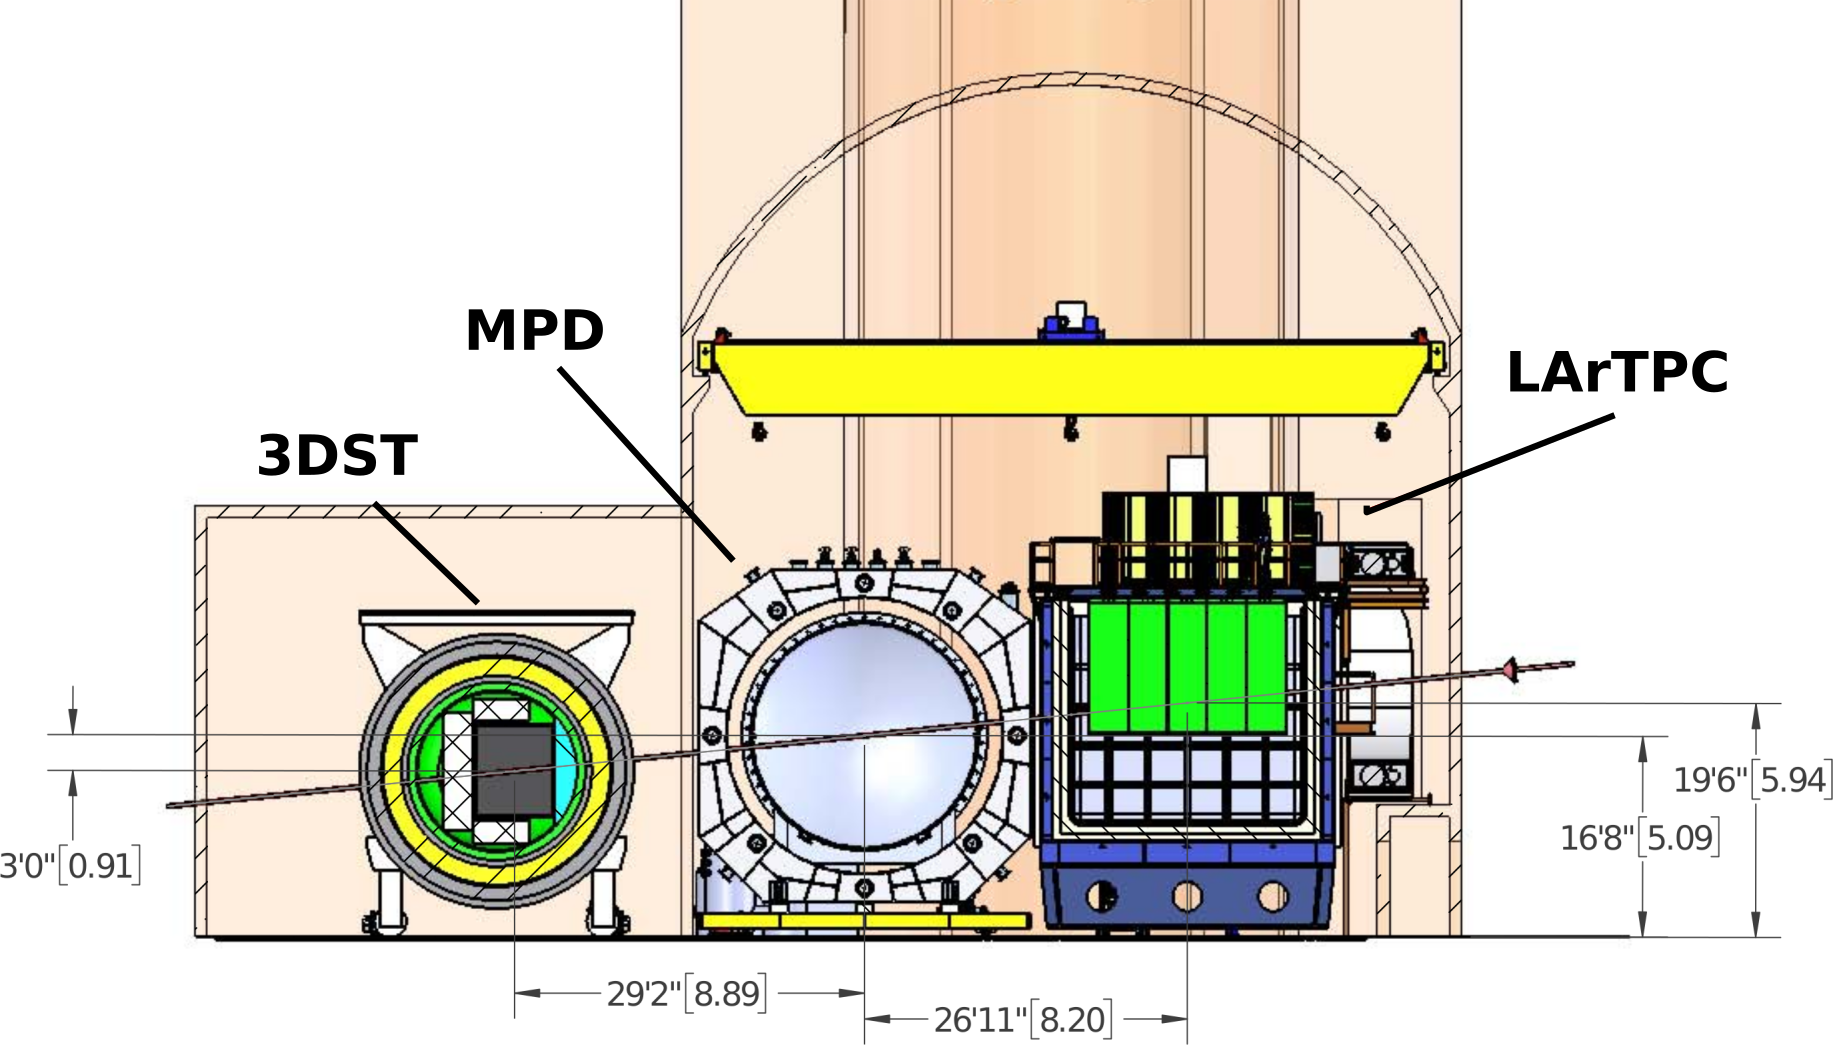
\includegraphics[width=0.7\textwidth]{pics/duneND.png}
	\caption[View of the near detector complex of DUNE]%
	{Lateral view of the near detector complex of DUNE.}
	\label{fig:duneND}
\end{figure}

A very sensitive FD alone, however, is not enough due to numerous uncertainties on the neutrino flux and cross-section parameters.
A smaller and closer detector, called near detector (ND), is therefore adopted to normalise %
the flux of neutrinos reaching the FD and to help cancel out many of the neutrino-nucleon cross-section systematics.
The DUNE ND will be placed \np{574}\,m from the target.
Its design is a hybrid concept, consisting of a small LArTPC placed in front of a magnetised high-pressure gaseous TPC~\cite{Abi:2020wmh}.
This module is complementary to the LArTPC, controlling escaping or below-threshold particles from the LArTPC, %
but is also capable of performing standalone measurement.
For its versatile nature, it is called Multi-Purpose Detector (MPD).
The subsystem LArTPC/MPD will be movable inside the ND hall\,---\,following the DUNE-PRISM concept~\cite{Abi:2020wmh}\,---\,for %
better profiling the neutrino flux at different angles.
There will be a third module, a 3D Scintillation Tracker (3DST), on-axis, to monitor %
the stability of the beam flux and neutron contamination.
The configuration is shown in \reffig{fig:duneND}.
Currently, the proposed fiducial volume for the LArTPC module is 36\,m\tapi{3} and 50\,t of LAr, %
employing the ArgonCube technology~\cite{Asaadi:2018xfh}, %
whereas the design for the MPD is based on the TPC of \mbox{ALICE}~\cite{Glassel:2004jv}.
It consists of a cylinder of 102\,m\tapi{3} with gas at a pressure of 10\,atm and a fiducial mass of~1\,t; %
the gas assumed for the study is a an 80--20 mixture of Ar--CH\tped{4}.
The 3DST is designed to have a fiducial mass of around \np{8.7}\,t of plastic scintillating material and %
wavelength shifting plates.
%($3\times2\times6$)\,m\tapi{3},
%and for the HPArFGT is ($3.5\times3.5\times6.4$)\,m\tapi{3}.
For this analysis, only the two core subdetectors, the LArTPC and the MPD, are taken into account.
The main difference between these two ND modules is that the gaseous TPC has a larger volume than the LArTPC.
This feature is favourable when studying rare events, like heavy neutrino decays, because more neutrinos enter the fiducial volume.
Furthermore, the lower density of the MPD helps reduce the number of neutrino scattering events, which are background to rare signatures.
Apart from volume and density differences and relative positions in the detector hall, %
the two ND units are assumed to have similar detection performances and to be on-axis; %
the magnetisation of the gaseous TPC is not considered for HNL discovery.
%Optical partitioning, short electron drift distance, and pixelated readout are features being taken in consideration to %
%improve the performance of the LArTPC to the anticipated high-rate environment %
%and the efficiency of reconstructing events at the near site.

Thanks to its proximity to the accelerator, the ND will be exposed to an extremely intense neutrino beam, %
with a flux peak around five million times greater than at the FD.
The Long Baseline Neutrino Facility (LBNF) at Fermilab will deploy a very energetic beam of protons, %
extracted from the Fermilab main injector and delivered to a graphite target.
The collision produces secondary particles, which are collimated by a focusing horn system and then decay forming a neutrino beam.
Assuming an 80\,GeV proton beam at 1.2\,MW for the first six years and at 2.4\,MW for a second set of six years~\cite{Abi:2018dnh}, 
the ND will collect a total of \np{2.65e22} protons on target (POT) over the lifespan of the experiment, %
running for the same amount of time in neutrino and antineutrino mode.
The ND will be placed on-axis for half of the total runtime, whereas it will be positioned %
at different angles off-axis for the remaining acquisition period, enacting the DUNE-PRISM concept.
The search for HNL decays can benefit to some extent with the detector positioned at off-axis angles, %
as the SM neutrino background is particularly reduced despite a lower signal rate.
However, the modelling of the neutrino beam profile at different angles using only %
information from the on-axis spectrum is not trivial.
Half of the total statistics will be collected with a reversed horn current configuration, %
but the parentage composition of the neutrino beam in $\cj{\nu}$-mode was not provided, %
as well as the off-axis beam flux.
In this work, just the on-axis configuration of the ND with a forward horn current configuration is considered, %
which would correspond to a quarter of the runtime, or \np{0.66e22}\,POT.
The same analysis of this study can nonetheless be applied equally to the beam in antineutrino mode, %
which should result in a sensitivity similar to the neutrino mode configuration, %
being wary of the different composition of the neutrino spectrum.
Even though a precise estimate of the DUNE ND sensitivity cannot be achieved, %
with the above caveats the total sensitivity to HNL\,---\,including off-axis angles and antineutrino mode beam\,---\,%
can be naively equivalent to six years of data taking, i.e.\ \np{1.32e22}\,POT, %
with the beam in neutrino mode and the ND on-axis.

%In this work we consider only the beam in the neutrino mode configuration, %
%which corresponds to half of the total runtime, or \np{1.32e22}\,POT.
%The same study of this article can be applied equally to the beam in reversed horn current configuration, %
%but its details are not available to us.
%Including the analysis for the beam in antineutrino mode should result in an increment on the overall sensitivity, %
%approximately a factor of two better.

%Moreover, the ND system could implement the $\nu$PRISM concept~\cite{Bhadra:2014oma}, which would make the detector %
%	movable, to take advantage of the monochromatic nature of the neutrino beam off-axis.

\subsection{Exposure}
\label{sec:exposure}

\begin{table}
	\centering
	\caption[Exposures of major beam dump experiments]%
		{Comparison between experiments mentioned in this work.
		Using PS191 as a reference unit, the exposure is defined as %
		POT$\times$Energy$\times$Volume$\times$Baseline\tapi{$-$2}, %
		where ``Energy'' is the proton beam energy.
		The NA62 and SHiP experiments are not directly comparable with SBND and DUNE ND, %
		in that different technologies are involved;
		the RICH detectors are adopted as fiducial volume for NA62, whereas %
		the volume of SHiP is estimated as the cone contained in the ``hidden sector'' vacuum vessel. 
		The volume is a driving feature in the definition of the total exposure and it is of utter importance %
		for searches of decay-in-flight events.}
	\label{tab:nd}
	\small
	\begin{tabular}{lccccc}
		\toprule
		&\textbf{PS191}	& \textbf{DUNE ND}& \textbf{SBND}	& \textbf{NA62} & \textbf{SHiP} \\
		\midrule
		Baseline& 128\,m		    & 574\,m			& 110\,m		    & 220\,m         & 60\,m          \\
		Volume  & 216\,m\tapi{3} & 150\,m\tapi{3} & 80\,m\tapi{3}  & 750\,m\tapi{3} & 590\,m\tapi{3} \\
		Energy	& 19.2\,GeV	    & 80\,GeV	    & 8\,GeV		    & 400\,GeV       & 400\,GeV       \\
		POT	    & \np{0.86e19}	& \np{1.32e22}	& \np{6.6e20}	& \np{3e18}     & \np{2e20}     \\
		\midrule
		Exposure& 1.0 	        & 220.9         & 16.4	        & 8.5           & 5820          \\
		\bottomrule
	\end{tabular}
\end{table}

A summary of the features of the ND system relevant for this analysis is reported in~\reftab{tab:nd}, %
where it is compared to other beam dump experiments: %
PS191~\cite{Bernardi:1985ny,Bernardi:1987ek}, SBND which is the detector of the SBN programme with the best sensitivity to %
HNL~\cite{Ballett:2016opr}, NA62~\cite{NA62:2017rwk}, and SHiP~\cite{Anelli:2015pba}.
The total exposure of the experiment is defined as the proton accelerator beam power, integrated over the total run time, %
and scaled by the volume of the detector over its baseline squared.
The beam power times the run time corresponds to the number of POT times the proton energy. 
With this definition, an exposure twelve times bigger is expected for the DUNE ND system with respect to SBND, %
and around two hundred times bigger than PS191.
Although NA62 and SHiP can be considered beam dump experiments, these experiments have a different design %
and use technologies not directly comparable to TPC and tracker experiments; %
they are reported here for thoroughness since they give competitive sensitivities to HNL searches.
The estimated exposure of NA62 is limited by its number of POT and by just one year of data taking; %
in spite of this, the experiment is optimised to study kaon decays and has good %
sensitivity to HNL~\cite{Drewes:2018irr}.
The SHiP experiment presents an exposure thirty times bigger than DUNE ND, but the detector is specifically %
designed to search for BSM physics, including heavy neutrinos~\cite{SHiP:2018xqw,Caputo:2016ojx}.
The decay-in-flight search hugely benefits from its 50\,m long decay vessel and short baseline.
On the collider physics frontier, the MATHUSLA~\cite{Curtin:2018mvb} and the FASER~\cite{Ariga:2018uku} experiments %
will perform a dedicated search for extremely weakly-interacting and long lived particles, %
like HNLs for which they present interesting sensitivity~\cite{Curtin:2018mvb, Kling:2018wct}.
MATHUSLA will be a \np{800e3}\,m\tapi{3} hodoscope placed on the surface above the ATLAS or the CMS detectors.
FASER will consist of a 10\,m cylindrical decay volume located 480\,m downstream of the ATLAS interaction point. 

\subsection{Flux prediction}
\label{sec:tauneutrino}

\begin{figure}[t]
	\centering
	\resizebox{.5\textwidth}{!}{% GNUPLOT: LaTeX picture with Postscript
\begingroup
  \makeatletter
  \providecommand\color[2][]{%
    \GenericError{(gnuplot) \space\space\space\@spaces}{%
      Package color not loaded in conjunction with
      terminal option `colourtext'%
    }{See the gnuplot documentation for explanation.%
    }{Either use 'blacktext' in gnuplot or load the package
      color.sty in LaTeX.}%
    \renewcommand\color[2][]{}%
  }%
  \providecommand\includegraphics[2][]{%
    \GenericError{(gnuplot) \space\space\space\@spaces}{%
      Package graphicx or graphics not loaded%
    }{See the gnuplot documentation for explanation.%
    }{The gnuplot epslatex terminal needs graphicx.sty or graphics.sty.}%
    \renewcommand\includegraphics[2][]{}%
  }%
  \providecommand\rotatebox[2]{#2}%
  \@ifundefined{ifGPcolor}{%
    \newif\ifGPcolor
    \GPcolortrue
  }{}%
  \@ifundefined{ifGPblacktext}{%
    \newif\ifGPblacktext
    \GPblacktexttrue
  }{}%
  % define a \g@addto@macro without @ in the name:
  \let\gplgaddtomacro\g@addto@macro
  % define empty templates for all commands taking text:
  \gdef\gplbacktext{}%
  \gdef\gplfronttext{}%
  \makeatother
  \ifGPblacktext
    % no textcolor at all
    \def\colorrgb#1{}%
    \def\colorgray#1{}%
  \else
    % gray or color?
    \ifGPcolor
      \def\colorrgb#1{\color[rgb]{#1}}%
      \def\colorgray#1{\color[gray]{#1}}%
      \expandafter\def\csname LTw\endcsname{\color{white}}%
      \expandafter\def\csname LTb\endcsname{\color{black}}%
      \expandafter\def\csname LTa\endcsname{\color{black}}%
      \expandafter\def\csname LT0\endcsname{\color[rgb]{1,0,0}}%
      \expandafter\def\csname LT1\endcsname{\color[rgb]{0,1,0}}%
      \expandafter\def\csname LT2\endcsname{\color[rgb]{0,0,1}}%
      \expandafter\def\csname LT3\endcsname{\color[rgb]{1,0,1}}%
      \expandafter\def\csname LT4\endcsname{\color[rgb]{0,1,1}}%
      \expandafter\def\csname LT5\endcsname{\color[rgb]{1,1,0}}%
      \expandafter\def\csname LT6\endcsname{\color[rgb]{0,0,0}}%
      \expandafter\def\csname LT7\endcsname{\color[rgb]{1,0.3,0}}%
      \expandafter\def\csname LT8\endcsname{\color[rgb]{0.5,0.5,0.5}}%
    \else
      % gray
      \def\colorrgb#1{\color{black}}%
      \def\colorgray#1{\color[gray]{#1}}%
      \expandafter\def\csname LTw\endcsname{\color{white}}%
      \expandafter\def\csname LTb\endcsname{\color{black}}%
      \expandafter\def\csname LTa\endcsname{\color{black}}%
      \expandafter\def\csname LT0\endcsname{\color{black}}%
      \expandafter\def\csname LT1\endcsname{\color{black}}%
      \expandafter\def\csname LT2\endcsname{\color{black}}%
      \expandafter\def\csname LT3\endcsname{\color{black}}%
      \expandafter\def\csname LT4\endcsname{\color{black}}%
      \expandafter\def\csname LT5\endcsname{\color{black}}%
      \expandafter\def\csname LT6\endcsname{\color{black}}%
      \expandafter\def\csname LT7\endcsname{\color{black}}%
      \expandafter\def\csname LT8\endcsname{\color{black}}%
    \fi
  \fi
    \setlength{\unitlength}{0.0500bp}%
    \ifx\gptboxheight\undefined%
      \newlength{\gptboxheight}%
      \newlength{\gptboxwidth}%
      \newsavebox{\gptboxtext}%
    \fi%
    \setlength{\fboxrule}{0.5pt}%
    \setlength{\fboxsep}{1pt}%
\begin{picture}(7200.00,5040.00)%
    \gplgaddtomacro\gplbacktext{%
      \csname LTb\endcsname%%
      \put(924,704){\makebox(0,0)[r]{\strut{}\np{e8}}}%
      \put(924,2285){\makebox(0,0)[r]{\strut{}\np{e9}}}%
      \put(924,3867){\makebox(0,0)[r]{\strut{}\np{e10}}}%
      \put(1056,484){\makebox(0,0){\strut{}0}}%
      \put(2526,484){\makebox(0,0){\strut{}5}}%
      \put(3996,484){\makebox(0,0){\strut{}10}}%
      \put(5465,484){\makebox(0,0){\strut{}15}}%
      \put(6935,484){\makebox(0,0){\strut{}20}}%
    }%
    \gplgaddtomacro\gplfronttext{%
      \csname LTb\endcsname%%
      \put(176,2761){\rotatebox{-270}{\makebox(0,0){\strut{}$\nu_e / \text{cm}^2 / \text{GeV}$}}}%
      \put(3995,154){\makebox(0,0){\strut{}Energy (GeV)}}%
      \csname LTb\endcsname%%
      \put(6318,4624){\makebox(0,0)[r]{\strut{}Total}}%
      \csname LTb\endcsname%%
      \put(6318,4360){\makebox(0,0)[r]{\strut{}$\pi$}}%
      \csname LTb\endcsname%%
      \put(6318,4096){\makebox(0,0)[r]{\strut{}$K$}}%
      \csname LTb\endcsname%%
      \put(6318,3832){\makebox(0,0)[r]{\strut{}$K^0$}}%
      \csname LTb\endcsname%%
      \put(6318,3568){\makebox(0,0)[r]{\strut{}$\mu$}}%
      \csname LTb\endcsname%%
      \put(6318,3304){\makebox(0,0)[r]{\strut{}$D_s$}}%
    }%
    \gplbacktext
    \put(0,0){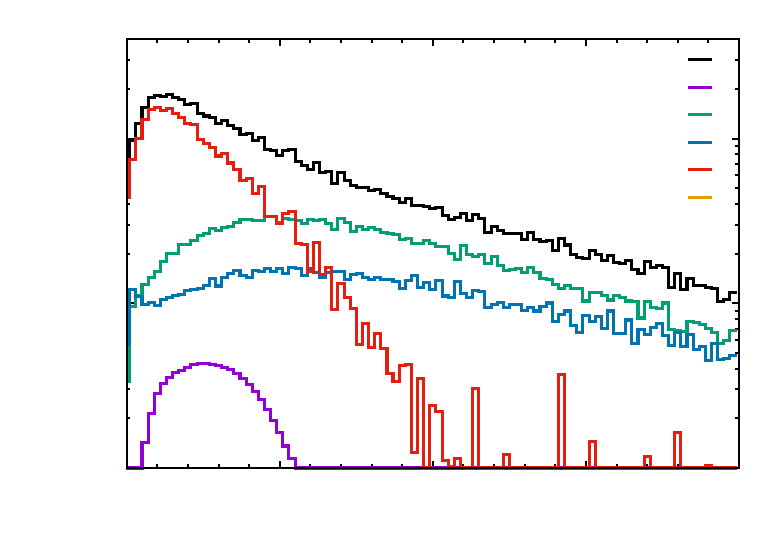
\includegraphics{pics/fluxnue}}%
    \gplfronttext
  \end{picture}%
\endgroup
}
	\hspace{-1em}
	\resizebox{.5\textwidth}{!}{% GNUPLOT: LaTeX picture with Postscript
\begingroup
  \makeatletter
  \providecommand\color[2][]{%
    \GenericError{(gnuplot) \space\space\space\@spaces}{%
      Package color not loaded in conjunction with
      terminal option `colourtext'%
    }{See the gnuplot documentation for explanation.%
    }{Either use 'blacktext' in gnuplot or load the package
      color.sty in LaTeX.}%
    \renewcommand\color[2][]{}%
  }%
  \providecommand\includegraphics[2][]{%
    \GenericError{(gnuplot) \space\space\space\@spaces}{%
      Package graphicx or graphics not loaded%
    }{See the gnuplot documentation for explanation.%
    }{The gnuplot epslatex terminal needs graphicx.sty or graphics.sty.}%
    \renewcommand\includegraphics[2][]{}%
  }%
  \providecommand\rotatebox[2]{#2}%
  \@ifundefined{ifGPcolor}{%
    \newif\ifGPcolor
    \GPcolortrue
  }{}%
  \@ifundefined{ifGPblacktext}{%
    \newif\ifGPblacktext
    \GPblacktexttrue
  }{}%
  % define a \g@addto@macro without @ in the name:
  \let\gplgaddtomacro\g@addto@macro
  % define empty templates for all commands taking text:
  \gdef\gplbacktext{}%
  \gdef\gplfronttext{}%
  \makeatother
  \ifGPblacktext
    % no textcolor at all
    \def\colorrgb#1{}%
    \def\colorgray#1{}%
  \else
    % gray or color?
    \ifGPcolor
      \def\colorrgb#1{\color[rgb]{#1}}%
      \def\colorgray#1{\color[gray]{#1}}%
      \expandafter\def\csname LTw\endcsname{\color{white}}%
      \expandafter\def\csname LTb\endcsname{\color{black}}%
      \expandafter\def\csname LTa\endcsname{\color{black}}%
      \expandafter\def\csname LT0\endcsname{\color[rgb]{1,0,0}}%
      \expandafter\def\csname LT1\endcsname{\color[rgb]{0,1,0}}%
      \expandafter\def\csname LT2\endcsname{\color[rgb]{0,0,1}}%
      \expandafter\def\csname LT3\endcsname{\color[rgb]{1,0,1}}%
      \expandafter\def\csname LT4\endcsname{\color[rgb]{0,1,1}}%
      \expandafter\def\csname LT5\endcsname{\color[rgb]{1,1,0}}%
      \expandafter\def\csname LT6\endcsname{\color[rgb]{0,0,0}}%
      \expandafter\def\csname LT7\endcsname{\color[rgb]{1,0.3,0}}%
      \expandafter\def\csname LT8\endcsname{\color[rgb]{0.5,0.5,0.5}}%
    \else
      % gray
      \def\colorrgb#1{\color{black}}%
      \def\colorgray#1{\color[gray]{#1}}%
      \expandafter\def\csname LTw\endcsname{\color{white}}%
      \expandafter\def\csname LTb\endcsname{\color{black}}%
      \expandafter\def\csname LTa\endcsname{\color{black}}%
      \expandafter\def\csname LT0\endcsname{\color{black}}%
      \expandafter\def\csname LT1\endcsname{\color{black}}%
      \expandafter\def\csname LT2\endcsname{\color{black}}%
      \expandafter\def\csname LT3\endcsname{\color{black}}%
      \expandafter\def\csname LT4\endcsname{\color{black}}%
      \expandafter\def\csname LT5\endcsname{\color{black}}%
      \expandafter\def\csname LT6\endcsname{\color{black}}%
      \expandafter\def\csname LT7\endcsname{\color{black}}%
      \expandafter\def\csname LT8\endcsname{\color{black}}%
    \fi
  \fi
    \setlength{\unitlength}{0.0500bp}%
    \ifx\gptboxheight\undefined%
      \newlength{\gptboxheight}%
      \newlength{\gptboxwidth}%
      \newsavebox{\gptboxtext}%
    \fi%
    \setlength{\fboxrule}{0.5pt}%
    \setlength{\fboxsep}{1pt}%
\begin{picture}(7200.00,5040.00)%
    \gplgaddtomacro\gplbacktext{%
      \csname LTb\endcsname%%
      \put(924,704){\makebox(0,0)[r]{\strut{}\np{e8}}}%
      \put(924,1527){\makebox(0,0)[r]{\strut{}\np{e9}}}%
      \put(924,2350){\makebox(0,0)[r]{\strut{}\np{e10}}}%
      \put(924,3173){\makebox(0,0)[r]{\strut{}\np{e11}}}%
      \put(924,3996){\makebox(0,0)[r]{\strut{}\np{e12}}}%
      \put(924,4819){\makebox(0,0)[r]{\strut{}\np{e13}}}%
      \put(1056,484){\makebox(0,0){\strut{}0}}%
      \put(2526,484){\makebox(0,0){\strut{}5}}%
      \put(3996,484){\makebox(0,0){\strut{}10}}%
      \put(5465,484){\makebox(0,0){\strut{}15}}%
      \put(6935,484){\makebox(0,0){\strut{}20}}%
    }%
    \gplgaddtomacro\gplfronttext{%
      \csname LTb\endcsname%%
      \put(176,2761){\rotatebox{-270}{\makebox(0,0){\strut{}$\nu_\mu / \text{cm}^2 / \text{GeV}$}}}%
      \put(3995,154){\makebox(0,0){\strut{}Energy (GeV)}}%
      \csname LTb\endcsname%%
      \put(6318,4624){\makebox(0,0)[r]{\strut{}Total}}%
      \csname LTb\endcsname%%
      \put(6318,4360){\makebox(0,0)[r]{\strut{}$\pi$}}%
      \csname LTb\endcsname%%
      \put(6318,4096){\makebox(0,0)[r]{\strut{}$K$}}%
      \csname LTb\endcsname%%
      \put(6318,3832){\makebox(0,0)[r]{\strut{}$K^0$}}%
      \csname LTb\endcsname%%
      \put(6318,3568){\makebox(0,0)[r]{\strut{}$\mu$}}%
      \csname LTb\endcsname%%
      \put(6318,3304){\makebox(0,0)[r]{\strut{}$D_s$}}%
    }%
    \gplbacktext
    \put(0,0){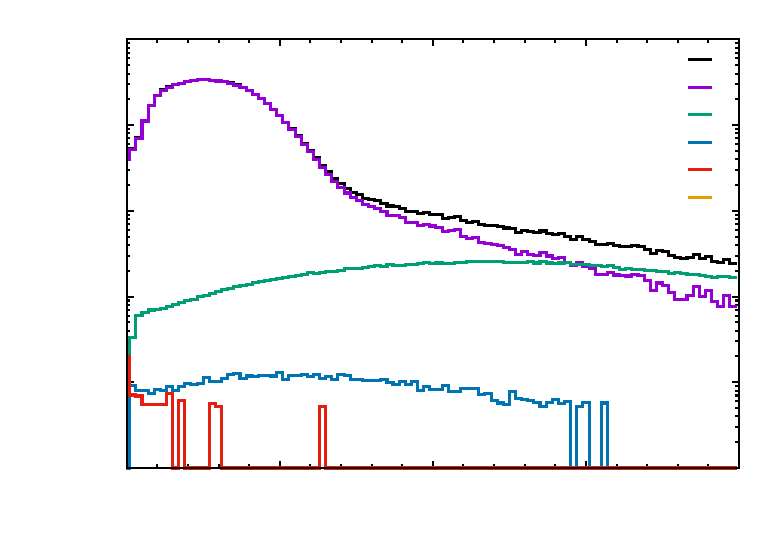
\includegraphics{pics/fluxnumu}}%
    \gplfronttext
  \end{picture}%
\endgroup
}
	\\
	\resizebox{.5\textwidth}{!}{% GNUPLOT: LaTeX picture with Postscript
\begingroup
  \makeatletter
  \providecommand\color[2][]{%
    \GenericError{(gnuplot) \space\space\space\@spaces}{%
      Package color not loaded in conjunction with
      terminal option `colourtext'%
    }{See the gnuplot documentation for explanation.%
    }{Either use 'blacktext' in gnuplot or load the package
      color.sty in LaTeX.}%
    \renewcommand\color[2][]{}%
  }%
  \providecommand\includegraphics[2][]{%
    \GenericError{(gnuplot) \space\space\space\@spaces}{%
      Package graphicx or graphics not loaded%
    }{See the gnuplot documentation for explanation.%
    }{The gnuplot epslatex terminal needs graphicx.sty or graphics.sty.}%
    \renewcommand\includegraphics[2][]{}%
  }%
  \providecommand\rotatebox[2]{#2}%
  \@ifundefined{ifGPcolor}{%
    \newif\ifGPcolor
    \GPcolortrue
  }{}%
  \@ifundefined{ifGPblacktext}{%
    \newif\ifGPblacktext
    \GPblacktexttrue
  }{}%
  % define a \g@addto@macro without @ in the name:
  \let\gplgaddtomacro\g@addto@macro
  % define empty templates for all commands taking text:
  \gdef\gplbacktext{}%
  \gdef\gplfronttext{}%
  \makeatother
  \ifGPblacktext
    % no textcolor at all
    \def\colorrgb#1{}%
    \def\colorgray#1{}%
  \else
    % gray or color?
    \ifGPcolor
      \def\colorrgb#1{\color[rgb]{#1}}%
      \def\colorgray#1{\color[gray]{#1}}%
      \expandafter\def\csname LTw\endcsname{\color{white}}%
      \expandafter\def\csname LTb\endcsname{\color{black}}%
      \expandafter\def\csname LTa\endcsname{\color{black}}%
      \expandafter\def\csname LT0\endcsname{\color[rgb]{1,0,0}}%
      \expandafter\def\csname LT1\endcsname{\color[rgb]{0,1,0}}%
      \expandafter\def\csname LT2\endcsname{\color[rgb]{0,0,1}}%
      \expandafter\def\csname LT3\endcsname{\color[rgb]{1,0,1}}%
      \expandafter\def\csname LT4\endcsname{\color[rgb]{0,1,1}}%
      \expandafter\def\csname LT5\endcsname{\color[rgb]{1,1,0}}%
      \expandafter\def\csname LT6\endcsname{\color[rgb]{0,0,0}}%
      \expandafter\def\csname LT7\endcsname{\color[rgb]{1,0.3,0}}%
      \expandafter\def\csname LT8\endcsname{\color[rgb]{0.5,0.5,0.5}}%
    \else
      % gray
      \def\colorrgb#1{\color{black}}%
      \def\colorgray#1{\color[gray]{#1}}%
      \expandafter\def\csname LTw\endcsname{\color{white}}%
      \expandafter\def\csname LTb\endcsname{\color{black}}%
      \expandafter\def\csname LTa\endcsname{\color{black}}%
      \expandafter\def\csname LT0\endcsname{\color{black}}%
      \expandafter\def\csname LT1\endcsname{\color{black}}%
      \expandafter\def\csname LT2\endcsname{\color{black}}%
      \expandafter\def\csname LT3\endcsname{\color{black}}%
      \expandafter\def\csname LT4\endcsname{\color{black}}%
      \expandafter\def\csname LT5\endcsname{\color{black}}%
      \expandafter\def\csname LT6\endcsname{\color{black}}%
      \expandafter\def\csname LT7\endcsname{\color{black}}%
      \expandafter\def\csname LT8\endcsname{\color{black}}%
    \fi
  \fi
    \setlength{\unitlength}{0.0500bp}%
    \ifx\gptboxheight\undefined%
      \newlength{\gptboxheight}%
      \newlength{\gptboxwidth}%
      \newsavebox{\gptboxtext}%
    \fi%
    \setlength{\fboxrule}{0.5pt}%
    \setlength{\fboxsep}{1pt}%
\begin{picture}(7200.00,5040.00)%
    \gplgaddtomacro\gplbacktext{%
      \csname LTb\endcsname%%
      \put(924,1079){\makebox(0,0)[r]{\strut{}\np{e9}}}%
      \put(924,2326){\makebox(0,0)[r]{\strut{}\np{e10}}}%
      \put(924,3572){\makebox(0,0)[r]{\strut{}\np{e11}}}%
      \put(924,4819){\makebox(0,0)[r]{\strut{}\np{e12}}}%
      \put(1056,484){\makebox(0,0){\strut{}0}}%
      \put(2526,484){\makebox(0,0){\strut{}5}}%
      \put(3996,484){\makebox(0,0){\strut{}10}}%
      \put(5465,484){\makebox(0,0){\strut{}15}}%
      \put(6935,484){\makebox(0,0){\strut{}20}}%
    }%
    \gplgaddtomacro\gplfronttext{%
      \csname LTb\endcsname%%
      \put(176,2761){\rotatebox{-270}{\makebox(0,0){\strut{}$\cj{\nu}_\mu / \text{cm}^2 / \text{GeV}$}}}%
      \put(3995,154){\makebox(0,0){\strut{}Energy (GeV)}}%
      \csname LTb\endcsname%%
      \put(6318,4624){\makebox(0,0)[r]{\strut{}Total}}%
      \csname LTb\endcsname%%
      \put(6318,4360){\makebox(0,0)[r]{\strut{}$\pi$}}%
      \csname LTb\endcsname%%
      \put(6318,4096){\makebox(0,0)[r]{\strut{}$K$}}%
      \csname LTb\endcsname%%
      \put(6318,3832){\makebox(0,0)[r]{\strut{}$K^0$}}%
      \csname LTb\endcsname%%
      \put(6318,3568){\makebox(0,0)[r]{\strut{}$\mu$}}%
    }%
    \gplbacktext
    \put(0,0){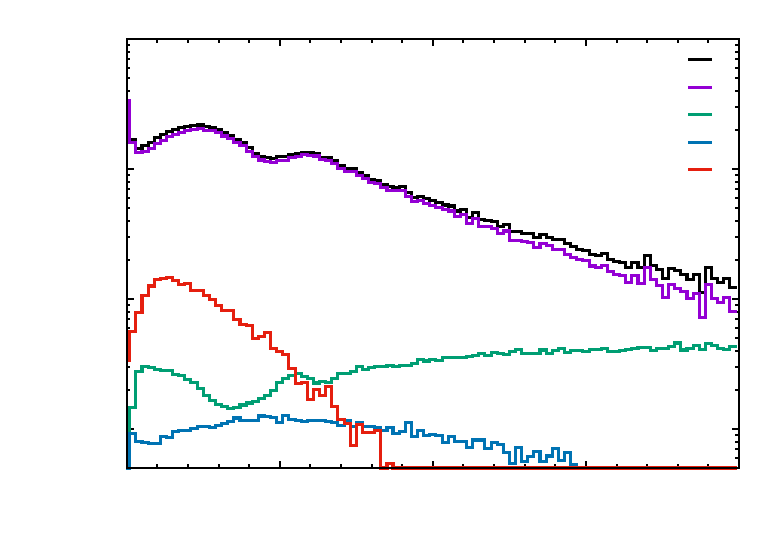
\includegraphics{pics/fluxnubar}}%
    \gplfronttext
  \end{picture}%
\endgroup
}
	\hspace{-1em}
	\resizebox{.5\textwidth}{!}{% GNUPLOT: LaTeX picture with Postscript
\begingroup
  \makeatletter
  \providecommand\color[2][]{%
    \GenericError{(gnuplot) \space\space\space\@spaces}{%
      Package color not loaded in conjunction with
      terminal option `colourtext'%
    }{See the gnuplot documentation for explanation.%
    }{Either use 'blacktext' in gnuplot or load the package
      color.sty in LaTeX.}%
    \renewcommand\color[2][]{}%
  }%
  \providecommand\includegraphics[2][]{%
    \GenericError{(gnuplot) \space\space\space\@spaces}{%
      Package graphicx or graphics not loaded%
    }{See the gnuplot documentation for explanation.%
    }{The gnuplot epslatex terminal needs graphicx.sty or graphics.sty.}%
    \renewcommand\includegraphics[2][]{}%
  }%
  \providecommand\rotatebox[2]{#2}%
  \@ifundefined{ifGPcolor}{%
    \newif\ifGPcolor
    \GPcolortrue
  }{}%
  \@ifundefined{ifGPblacktext}{%
    \newif\ifGPblacktext
    \GPblacktexttrue
  }{}%
  % define a \g@addto@macro without @ in the name:
  \let\gplgaddtomacro\g@addto@macro
  % define empty templates for all commands taking text:
  \gdef\gplbacktext{}%
  \gdef\gplfronttext{}%
  \makeatother
  \ifGPblacktext
    % no textcolor at all
    \def\colorrgb#1{}%
    \def\colorgray#1{}%
  \else
    % gray or color?
    \ifGPcolor
      \def\colorrgb#1{\color[rgb]{#1}}%
      \def\colorgray#1{\color[gray]{#1}}%
      \expandafter\def\csname LTw\endcsname{\color{white}}%
      \expandafter\def\csname LTb\endcsname{\color{black}}%
      \expandafter\def\csname LTa\endcsname{\color{black}}%
      \expandafter\def\csname LT0\endcsname{\color[rgb]{1,0,0}}%
      \expandafter\def\csname LT1\endcsname{\color[rgb]{0,1,0}}%
      \expandafter\def\csname LT2\endcsname{\color[rgb]{0,0,1}}%
      \expandafter\def\csname LT3\endcsname{\color[rgb]{1,0,1}}%
      \expandafter\def\csname LT4\endcsname{\color[rgb]{0,1,1}}%
      \expandafter\def\csname LT5\endcsname{\color[rgb]{1,1,0}}%
      \expandafter\def\csname LT6\endcsname{\color[rgb]{0,0,0}}%
      \expandafter\def\csname LT7\endcsname{\color[rgb]{1,0.3,0}}%
      \expandafter\def\csname LT8\endcsname{\color[rgb]{0.5,0.5,0.5}}%
    \else
      % gray
      \def\colorrgb#1{\color{black}}%
      \def\colorgray#1{\color[gray]{#1}}%
      \expandafter\def\csname LTw\endcsname{\color{white}}%
      \expandafter\def\csname LTb\endcsname{\color{black}}%
      \expandafter\def\csname LTa\endcsname{\color{black}}%
      \expandafter\def\csname LT0\endcsname{\color{black}}%
      \expandafter\def\csname LT1\endcsname{\color{black}}%
      \expandafter\def\csname LT2\endcsname{\color{black}}%
      \expandafter\def\csname LT3\endcsname{\color{black}}%
      \expandafter\def\csname LT4\endcsname{\color{black}}%
      \expandafter\def\csname LT5\endcsname{\color{black}}%
      \expandafter\def\csname LT6\endcsname{\color{black}}%
      \expandafter\def\csname LT7\endcsname{\color{black}}%
      \expandafter\def\csname LT8\endcsname{\color{black}}%
    \fi
  \fi
    \setlength{\unitlength}{0.0500bp}%
    \ifx\gptboxheight\undefined%
      \newlength{\gptboxheight}%
      \newlength{\gptboxwidth}%
      \newsavebox{\gptboxtext}%
    \fi%
    \setlength{\fboxrule}{0.5pt}%
    \setlength{\fboxsep}{1pt}%
\begin{picture}(7200.00,5040.00)%
    \gplgaddtomacro\gplbacktext{%
      \csname LTb\endcsname%%
      \put(924,704){\makebox(0,0)[r]{\strut{}\np{1}}}%
      \put(924,1733){\makebox(0,0)[r]{\strut{}\np{10}}}%
      \put(924,2762){\makebox(0,0)[r]{\strut{}\np{e2}}}%
      \put(924,3790){\makebox(0,0)[r]{\strut{}\np{e3}}}%
      \put(924,4819){\makebox(0,0)[r]{\strut{}\np{e4}}}%
      \put(1056,484){\makebox(0,0){\strut{}0}}%
      \put(2526,484){\makebox(0,0){\strut{}5}}%
      \put(3996,484){\makebox(0,0){\strut{}10}}%
      \put(5465,484){\makebox(0,0){\strut{}15}}%
      \put(6935,484){\makebox(0,0){\strut{}20}}%
    }%
    \gplgaddtomacro\gplfronttext{%
      \csname LTb\endcsname%%
      \put(308,2761){\rotatebox{-270}{\makebox(0,0){\strut{}$\overset{(-)}{\nu}_\tau / \text{cm}^2 / \text{GeV}$}}}%
      \put(3995,154){\makebox(0,0){\strut{}Energy (GeV)}}%
      \csname LTb\endcsname%%
      \put(6318,4624){\makebox(0,0)[r]{\strut{}$D_s\to\nu_\tau$}}%
      \csname LTb\endcsname%%
      \put(6318,4360){\makebox(0,0)[r]{\strut{}$\tau\to\cj{\nu}_\tau e$}}%
      \csname LTb\endcsname%%
      \put(6318,4096){\makebox(0,0)[r]{\strut{}$\tau\to\cj{\nu}_\tau \mu$}}%
      \csname LTb\endcsname%%
      \put(6318,3832){\makebox(0,0)[r]{\strut{}$\tau\to\cj{\nu}_\tau \pi$}}%
      \csname LTb\endcsname%%
      \put(6318,3568){\makebox(0,0)[r]{\strut{}$\tau\to\cj{\nu}_\tau \pi\pi^0$}}%
    }%
    \gplbacktext
    \put(0,0){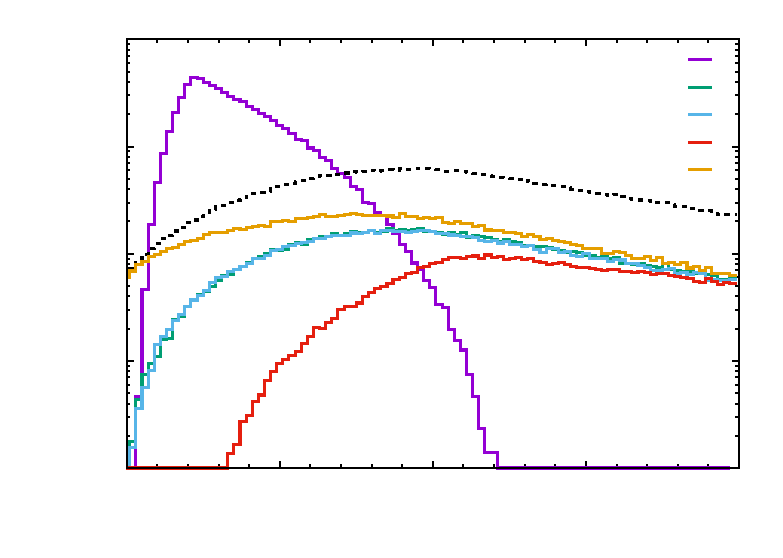
\includegraphics{pics/fluxnutau}}%
    \gplfronttext
  \end{picture}%
\endgroup
}
	\caption[Prediction of neutrino fluxes at the near detector of DUNE]%
		{The prediction of neutrino fluxes, in neutrino mode, divided by parentage at the ND are shown above, %
		normalised to \np{e20}\,POT.
		The $\nu_e$ component (top left) predominately originates from $\mu^+$ decays;
		kaon decays are responsible for the high energy part of the spectrum.
		The $\nu_\mu$ component (top right) obtains its main contribution from $\pi^+$ decays at low energies, %
		whereas the $K^+$ decays are accountable for the long tail of the spectrum.
		Contributions from $D_s^+$ decay are out of scale for both $\nu_e$ and $\nu_\mu$.
		The distribution of the $\cj{\nu}_\mu$ component (bottom left) is due to %
		negative charged secondary particles which are not successfully deflected by the horn system;
		the muon contribution is much more relevant than for the $\nu_\mu$ component.
		The $\nu_\tau$ component (bottom right) is only sourced from $D_s$ decays and presents a prominent peak at low energies, %
		whereas the $\cj{\nu}_\tau$ are produced in $\tau^+$ lepton decays.
		The dotted black line is the total $\cj{\nu}_\tau$ component of the flux.}
	\label{fig:fluxes}
\end{figure}

%A powerful proton beam is responsible for the very intense neutrino flux at the LBNF facility.
The study of HNL requires the various components of the flux by parentage to be known separately, %
as explained in \refsec{sec:production}.
Only the beam operating with a forward horn current is considered here.
Positively charged secondary particles are therefore selected at the target and this results %
in a beam dominantly made of neutrinos with a smaller component of antineutrinos.
The flux predictions for $\nu_e$, $\nu_\mu$, and $\cj{\nu}_\mu$ at DUNE, provided by \refref{LauraFields} for the reference beam, %
are shown in~\reffig{fig:fluxes} subdivided in their parent components.
The $\cj{\nu}_e$ component was not provided.
The $\nu_\mu$ flux is the dominant component and is principally originated %
by pion decays, whilst its long tail comes from kaon decays.
Unsuccessfully deflected negative particles, like $\pi^-$ or $K^-$, and the $\mu^+$ are the main contributors %
to the $\cj{\nu}_\mu$ components, and $\nu_e$ comes predominately from muon decays %
and both $K^+$ and $K^0$ decays.
The energy range considered is limited to $E < 20\,\text{GeV}$, because it is the most intense region of the flux %
and, as it will be explained in~\refsec{sec:numevt}, the most relevant for this study.

\begin{figure}[t]
	\centering
	\resizebox{\linewidth}{!}{% GNUPLOT: LaTeX picture with Postscript
\begingroup
  \makeatletter
  \providecommand\color[2][]{%
    \GenericError{(gnuplot) \space\space\space\@spaces}{%
      Package color not loaded in conjunction with
      terminal option `colourtext'%
    }{See the gnuplot documentation for explanation.%
    }{Either use 'blacktext' in gnuplot or load the package
      color.sty in LaTeX.}%
    \renewcommand\color[2][]{}%
  }%
  \providecommand\includegraphics[2][]{%
    \GenericError{(gnuplot) \space\space\space\@spaces}{%
      Package graphicx or graphics not loaded%
    }{See the gnuplot documentation for explanation.%
    }{The gnuplot epslatex terminal needs graphicx.sty or graphics.sty.}%
    \renewcommand\includegraphics[2][]{}%
  }%
  \providecommand\rotatebox[2]{#2}%
  \@ifundefined{ifGPcolor}{%
    \newif\ifGPcolor
    \GPcolortrue
  }{}%
  \@ifundefined{ifGPblacktext}{%
    \newif\ifGPblacktext
    \GPblacktexttrue
  }{}%
  % define a \g@addto@macro without @ in the name:
  \let\gplgaddtomacro\g@addto@macro
  % define empty templates for all commands taking text:
  \gdef\gplbacktext{}%
  \gdef\gplfronttext{}%
  \makeatother
  \ifGPblacktext
    % no textcolor at all
    \def\colorrgb#1{}%
    \def\colorgray#1{}%
  \else
    % gray or color?
    \ifGPcolor
      \def\colorrgb#1{\color[rgb]{#1}}%
      \def\colorgray#1{\color[gray]{#1}}%
      \expandafter\def\csname LTw\endcsname{\color{white}}%
      \expandafter\def\csname LTb\endcsname{\color{black}}%
      \expandafter\def\csname LTa\endcsname{\color{black}}%
      \expandafter\def\csname LT0\endcsname{\color[rgb]{1,0,0}}%
      \expandafter\def\csname LT1\endcsname{\color[rgb]{0,1,0}}%
      \expandafter\def\csname LT2\endcsname{\color[rgb]{0,0,1}}%
      \expandafter\def\csname LT3\endcsname{\color[rgb]{1,0,1}}%
      \expandafter\def\csname LT4\endcsname{\color[rgb]{0,1,1}}%
      \expandafter\def\csname LT5\endcsname{\color[rgb]{1,1,0}}%
      \expandafter\def\csname LT6\endcsname{\color[rgb]{0,0,0}}%
      \expandafter\def\csname LT7\endcsname{\color[rgb]{1,0.3,0}}%
      \expandafter\def\csname LT8\endcsname{\color[rgb]{0.5,0.5,0.5}}%
    \else
      % gray
      \def\colorrgb#1{\color{black}}%
      \def\colorgray#1{\color[gray]{#1}}%
      \expandafter\def\csname LTw\endcsname{\color{white}}%
      \expandafter\def\csname LTb\endcsname{\color{black}}%
      \expandafter\def\csname LTa\endcsname{\color{black}}%
      \expandafter\def\csname LT0\endcsname{\color{black}}%
      \expandafter\def\csname LT1\endcsname{\color{black}}%
      \expandafter\def\csname LT2\endcsname{\color{black}}%
      \expandafter\def\csname LT3\endcsname{\color{black}}%
      \expandafter\def\csname LT4\endcsname{\color{black}}%
      \expandafter\def\csname LT5\endcsname{\color{black}}%
      \expandafter\def\csname LT6\endcsname{\color{black}}%
      \expandafter\def\csname LT7\endcsname{\color{black}}%
      \expandafter\def\csname LT8\endcsname{\color{black}}%
    \fi
  \fi
    \setlength{\unitlength}{0.0500bp}%
    \ifx\gptboxheight\undefined%
      \newlength{\gptboxheight}%
      \newlength{\gptboxwidth}%
      \newsavebox{\gptboxtext}%
    \fi%
    \setlength{\fboxrule}{0.5pt}%
    \setlength{\fboxsep}{1pt}%
\begin{picture}(14400.00,5040.00)%
    \gplgaddtomacro\gplbacktext{%
      \csname LTb\endcsname%%
      \put(444,440){\makebox(0,0)[r]{\strut{}\np{10}}}%
      \put(444,1509){\makebox(0,0)[r]{\strut{}\np{e2}}}%
      \put(444,2579){\makebox(0,0)[r]{\strut{}\np{e3}}}%
      \put(444,3648){\makebox(0,0)[r]{\strut{}\np{e4}}}%
      \put(444,4717){\makebox(0,0)[r]{\strut{}\np{e5}}}%
      \put(576,220){\makebox(0,0){\strut{}$0$}}%
      \put(2336,220){\makebox(0,0){\strut{}$5$}}%
      \put(4095,220){\makebox(0,0){\strut{}$10$}}%
    }%
    \gplgaddtomacro\gplfronttext{%
      \csname LTb\endcsname%%
      \put(-172,2739){\rotatebox{-270}{\makebox(0,0){\strut{}$\nu_\tau$/cm\tapi{2}/GeV}}}%
      \put(2687,-110){\makebox(0,0){\strut{}Energy (GeV)}}%
      \csname LTb\endcsname%%
      \put(4182,4844){\makebox(0,0)[r]{\strut{}0 MeV}}%
      \csname LTb\endcsname%%
      \put(4182,4580){\makebox(0,0)[r]{\strut{}100 MeV}}%
      \csname LTb\endcsname%%
      \put(4182,4316){\makebox(0,0)[r]{\strut{}150 MeV}}%
      \csname LTb\endcsname%%
      \put(4182,4052){\makebox(0,0)[r]{\strut{}180 MeV}}%
      \csname LTb\endcsname%%
      \put(4182,3788){\makebox(0,0)[r]{\strut{}190 MeV}}%
    }%
    \gplgaddtomacro\gplbacktext{%
      \csname LTb\endcsname%%
      \put(5820,440){\makebox(0,0)[r]{\strut{}0.8}}%
      \put(5820,1590){\makebox(0,0)[r]{\strut{}0.85}}%
      \put(5820,2740){\makebox(0,0)[r]{\strut{}0.9}}%
      \put(5820,3889){\makebox(0,0)[r]{\strut{}0.95}}%
      \put(5820,5039){\makebox(0,0)[r]{\strut{}1}}%
      \put(5952,220){\makebox(0,0){\strut{}$0$}}%
      \put(6936,220){\makebox(0,0){\strut{}$0.5$}}%
      \put(7920,220){\makebox(0,0){\strut{}$1$}}%
      \put(8903,220){\makebox(0,0){\strut{}$1.5$}}%
      \put(9887,220){\makebox(0,0){\strut{}$2$}}%
    }%
    \gplgaddtomacro\gplfronttext{%
      \csname LTb\endcsname%%
      \put(5072,2739){\rotatebox{-270}{\makebox(0,0){\strut{}Factor}}}%
      \put(7919,-110){\makebox(0,0){\strut{}Mass $m_N$ (GeV)}}%
      \csname LTb\endcsname%%
      \put(9270,4844){\makebox(0,0)[r]{\strut{}$\tau \to \cj{\nu}_\tau e$}}%
      \csname LTb\endcsname%%
      \put(9270,4580){\makebox(0,0)[r]{\strut{}$\tau \to \cj{\nu}_\tau \mu$}}%
      \csname LTb\endcsname%%
      \put(9270,4316){\makebox(0,0)[r]{\strut{}$\tau \to \cj{\nu}_\tau \pi$}}%
      \csname LTb\endcsname%%
      \put(9270,4052){\makebox(0,0)[r]{\strut{}$\tau \to \cj{\nu}_\tau \pi \pi^0$}}%
    }%
    \gplgaddtomacro\gplbacktext{%
      \csname LTb\endcsname%%
      \put(10332,440){\makebox(0,0)[r]{\strut{}0}}%
      \put(10332,1276){\makebox(0,0)[r]{\strut{}0.2}}%
      \put(10332,2112){\makebox(0,0)[r]{\strut{}0.4}}%
      \put(10332,2949){\makebox(0,0)[r]{\strut{}0.6}}%
      \put(10332,3785){\makebox(0,0)[r]{\strut{}0.8}}%
      \put(10332,4621){\makebox(0,0)[r]{\strut{}1}}%
      \put(10464,220){\makebox(0,0){\strut{}$0$}}%
      \put(11448,220){\makebox(0,0){\strut{}$0.5$}}%
      \put(12432,220){\makebox(0,0){\strut{}$1$}}%
      \put(13415,220){\makebox(0,0){\strut{}$1.5$}}%
      \put(14399,220){\makebox(0,0){\strut{}$2$}}%
    }%
    \gplgaddtomacro\gplfronttext{%
      \csname LTb\endcsname%%
      \put(12431,-110){\makebox(0,0){\strut{}Mass $m_N$ (GeV)}}%
      \csname LTb\endcsname%%
      \put(13782,4844){\makebox(0,0)[r]{\strut{}$\tau \to \cj{\nu}_\tau e$}}%
      \csname LTb\endcsname%%
      \put(13782,4580){\makebox(0,0)[r]{\strut{}$\tau \to \cj{\nu}_\tau \mu$}}%
      \csname LTb\endcsname%%
      \put(13782,4316){\makebox(0,0)[r]{\strut{}$\tau \to \cj{\nu}_\tau \pi$}}%
      \csname LTb\endcsname%%
      \put(13782,4052){\makebox(0,0)[r]{\strut{}$\tau \to \cj{\nu}_\tau \pi \pi^0$}}%
    }%
    \gplbacktext
    \put(0,0){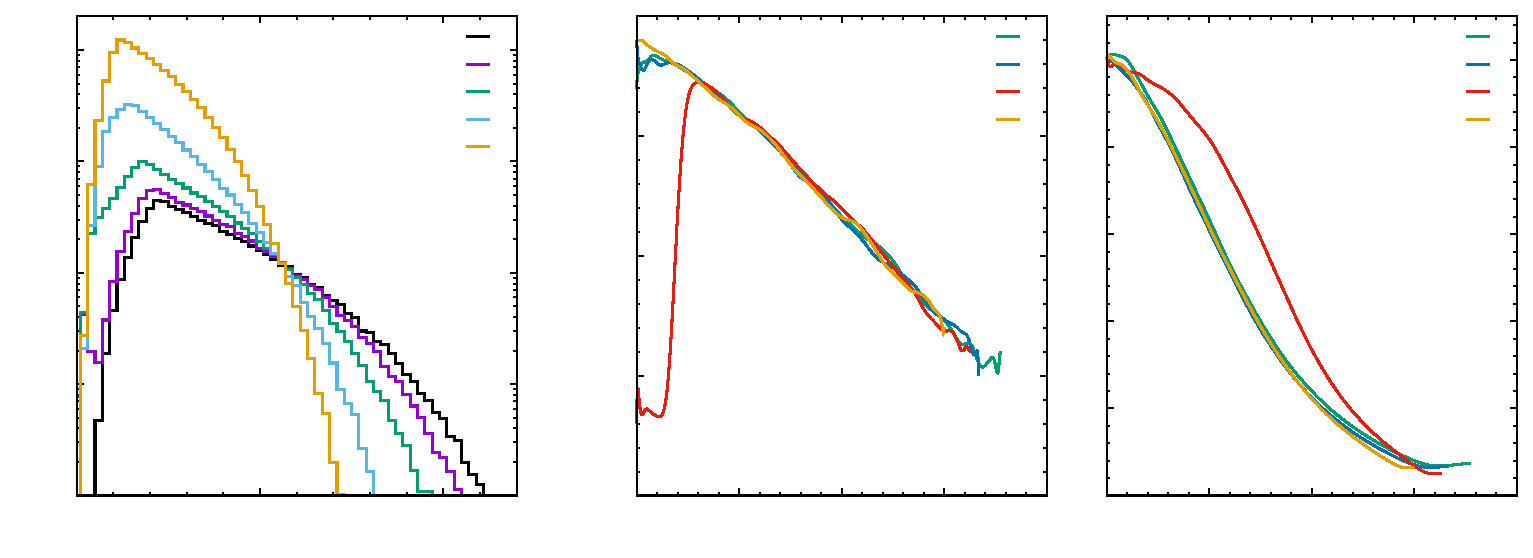
\includegraphics{pics/modmulti}}%
    \gplfronttext
  \end{picture}%
\endgroup
}
	\caption[Fluxes of heavy neutrinos from the decay channel $D_s^+\to \tau^+ N$]%
		{The fluxes of heavy neutrinos from $D_s^+\to \tau^+ N$ (left) are presented %
		for different neutrino masses and normalised to \np{e20}~POT at the ND.
		Only phase space effects are considered here.
		For each different value of the neutrino mass, information on the start and end point of the spectrum %
		and the peak of the flux are extracted and used to reshape the $\nu_\tau$ spectrum.
		The distortion factors used to build the heavy neutrino flux from mixing with $\cj{\nu}_\tau$ are also shown: %
		the energy range normalised to 20\,GeV (middle) and the inverse of the rescaled distribution peak (right). }
	\label{fig:taudist}
\end{figure}

An albeit-small flux of HNLs with masses above the kaon one is nonetheless expected.
This could be inferred from the $\nu_\tau$ flux, but this is not available in the literature.
In fact, the lightest meson with an interesting decay width to tau neutrinos is the charmed-strange meson~$D_s^+$, %
which has a mass $m_{D_s} = \np{1968.34}\pm\np{0.07}$\,MeV~\cite{Tanabashi:2018oca}.
It decays mostly into $\tau^+ \nu_\tau$ with a branching ratio of $(\np{5.48}\pm\np{0.23})$\,\%.
HNL with masses above the $K^0$ can be produced via the tau mixing, but more importantly via %
the muonic and electronic ones which are enhanced, as shown in \refsec{sec:production}.
The meson $D^+$ also decays into $\tau^+ \nu_\tau$, but being lighter than the $D_s^+$, %
the decay is disfavoured by the smaller phase space, with a branching ratio~50 times smaller.
This meson presents three-body decay channels into $\nu_e$ and $\nu_\mu$ with much higher branching ratio, %
but there is no enhancement for such channels into HNL, as explained in \refsec{sec:production}, and so these subdominant components %
are not taken in account in the present study.
%However, HNL with masses above the $K^0$ mass can only be produced by the decays of $D^+$ and $D_s^+$, %
%and the production of massive neutrinos could be enhanced, especially if produced via the $|U_{e 4}|^2$ mixing.
%{\color{red} What about the decay of $D^+$?? The considerations of it being disfavoured because of phase space would not apply to decay into N and muons or N and electron, which are enhanced compared to the standard case.}
%We make an estimate of the $\nu_\tau$ spectrum, starting from the $D_s^+$ production by %
%an 80\,GeV proton beam hitting a fixed graphite target.
The proton beam has a relatively low energy for producing charm quarks with a high cross-section, %
so the prediction of $\nu_\tau$ has not been carried out by the collaboration.
For the reasons stated above, a prediction for the $D_s^+$ production is carried out, %
assuming an 80\,GeV proton beam hitting a fixed graphite target.
The distribution at the production site will be then used to estimate the $\nu_\tau$ flux at the ND system.
In the literature, the following parametrisation has been successfully used to describe %
the charm meson production in proton--proton collision in the centre of mass frame~\cite{Ammar:1988ta}
\begin{equation}
	\label{eq:dsflux}
	\frac{\dd[2]{\sigma}}{\dd{x_F}\dd{p_T^2}} \sim (1-|x_F|)^n e^{-b p_T^2}~,
\end{equation}
where $x_F = 2 p_z/\sqrt{s}$, with $p_z$ the longitudinal momentum in the CM frame. %
The parameters $n$ and $b$ were fitted from the E769 experiment and found to be %
$n = \np{6.1}\pm\np{0.7}$ and \mbox{$b = \np{1.08}\pm\np{0.09}$}~\cite{Alves:1996qz}.
It is reasonable to assume that the $D_s^+$ meson production at the target follows the same distribution.
With the help of a custom Monte Carlo simulation, the $D_s^+$ four-momenta are generated starting from~\refeq{eq:dsflux} %
and simulate the meson decay and the subsequent tau decays.
A key simplification here is that because of the short lifetime of the $D_s^+$ and $\tau^+$, %
of the order of \np{e-13}\,s, their path is not affected by the horn system nor by interactions with other accelerator components. 
This results in no focusing of these secondary particles, and so only neutrinos emitted %
within the geometric acceptance of the ND are considered to form the $\nu_\tau$ and $\cj{\nu}_\tau$ spectrum.
The overall normalisation comes from an open charm calculation (see~\refapp{cha:opencc} for details): %
the number of $D_s^+$ per POT is found to be $(2.8 \pm 0.2) \times \np{e-6}$.
The result of the simulation is reported in \reffig{fig:fluxes}, %
where the different contributions to the $\nu_\tau$ spectrum are shown.
Thanks to the large number of POTs in DUNE, the total number of $D_s^+$ mesons produced is comparable %
to other dedicated experiments~\cite{Alekhin:2015byh}; %
however, the beamline design is not optimised for heavy mesons production %
and the $\nu_\tau$ flux seen at the ND is strongly attenuated.%: %
%according to our simulation, only \np{0.13}\,\% of the neutrinos produced at the target reaches the ND.

Having knowledge of the parent meson distribution, the production of nearly-sterile neutrinos %
are directly simulated from the $D_s$ decays.
The spectrum of heavy neutrinos is distorted when their mass approaches the various phase space thresholds, %
which appears as a further enhancement of the flux. 
This is because heavier neutrinos are more easily boosted inside the geometric acceptance of the detector.
Besides the peak height, the start and the end point of the energy flux are also affected,
as illustrated in~\reffig{fig:taudist} where the enhancement discussed in \refsec{sec:production} is not included.
The distribution of heavy neutrinos from $\tau$ decays also changes with the neutrino mass.
These effects are taken in account by modifying the scaled neutrino flux using information retrieved by the $\nu_\tau$ and $\cj{\nu}_\tau$~simulation. 


\section{Simulation of events at DUNE ND}
\label{sec:experiment}

\begin{table}
	\newcommand{\us}{\hphantom{${}^0$}}
	\newcommand{\ms}{\hphantom{${}^-$}}
	\caption[Expected rates for CC and NC interaction in the near detector of DUNE]%
		{The expected rates for CC and NC interaction in the near detector are presented here, normalised to \np{e20}\,POT.
		The values were computed starting from~\refeq{eq:numev}, convolving the fluxes of~\reffig{fig:fluxes} 
		with the CC and NC cross-section predictions from GENIE~\cite{Andreopoulos:2009rq}.
		Detector efficiencies are not applied.
		The first columns show the total number of events per tonne of argon, the second ones %
		the proportion of CC or NC events with respect to the totality, and the last columns the event frequencies %
		assuming \np{1e14}\,POT/s.}
	\label{tab:rate}
	\centering
	\small
	\iffalse
	\begin{tabular}{lrrrrrr}
		\toprule
		& \multicolumn{3}{c}{CC events}	&  \multicolumn{3}{c}{NC events}	\\
		%\midrule
		\cmidrule(lr){2-4} \cmidrule(lr){5-7}
		& Per tonne	& Ratio		& Rate (Hz)	& Per tonne 	& Ratio	& Rate (Hz)	\\
		\cmidrule(lr){2-4} \cmidrule(lr){5-7}
		%\midrule
		$\nu_e$		    & \np{3.0e3}\ms	& 75.6\,\%	& \np{152e-3}\us& \np{1.0e3}\ms	& 24.4\,\%	& \np{48.9e-3}\us	\\
		$\nu_\mu$	    & \np{236e3}\ms	& 75.2\,\%	& \np{12.0e0}\ms\us& \np{77.8e3}\ms& 24.8\,\%	& \np{3.95e0}\ms\us	\\
		$\cj{\nu_\mu}$	& \np{17.7e3}\ms& 70.9\,\%	& \np{898e-3}\us	& \np{7.2e3}\ms	& 29.1\,\%	& \np{368e-3}\us	\\
		$\nu_\tau$	    & \np{1.6e-5}	& 17.1\,\%	& \np{8.3e-10}	& \np{7.9e-5}	& 82.9\,\%	& \np{4.0e-10}	\\
		$\cj{\nu_\tau}$	& \np{5.2e-5}	& 45.3\,\%	& \np{2.6e-9}\us	& \np{6.1e-5}	& 54.7\,\%	& \np{3.0e-9}\us	\\
		\bottomrule
	\end{tabular}
	\fi
	\begin{tabular}{lrrr@{\,}lrrr@{\,}l} 
		\toprule
		& \multicolumn{3}{c}{CC events}	&  \multicolumn{3}{c}{NC events}	\\
		%\midrule
		\cmidrule(lr){2-5} \cmidrule(lr){6-9}
		& Per tonne	& Ratio		& \multicolumn{2}{c}{Rate (Hz)}	& Per tonne 	& Ratio	& \multicolumn{2}{c}{Rate (Hz)}	\\
		\cmidrule(lr){2-5} \cmidrule(lr){6-9}
		%\midrule
	$\nu_e$		    & %
	\np{3.0e3}\ms	& 75.6\,\%	& 152  & $\times\,10^{-3}$ & \np{1.0e3}\ms  & 24.4\,\% & 48.9 & $\times\,10^{-3}$	\\
	$\nu_\mu$	    & %
	\np{236e3}\ms	& 75.2\,\%	& 12.0 &                 & \np{77.8e3}\ms & 24.8\,\% & 3.95 &                  	\\
	$\cj{\nu_\mu}$	& %
	\np{17.7e3}\ms& 70.9\,\%	& 898  & $\times\,10^{-3}$ & \np{7.2e3}\ms  & 29.1\,\% & 368 & $\times\,10^{-3}$	\\
	$\nu_\tau$	    & %
	\np{1.6e-5}	& 17.1\,\%      & 8.3  & $\times\,10^{-10}$& \np{7.9e-5}    & 82.9\,\% & 4.0 & $\times\,10^{-10}$	\\
	$\cj{\nu_\tau}$	& %
	\np{5.2e-5}	& 45.3\,\%      & 2.6  & $\times\,10^{-3}$ & \np{6.1e-5}    & 54.7\,\% & 3.0 & $\times\,10^{-9}$	\\
		\bottomrule
	\end{tabular}
\end{table}

The number of SM neutrino--nucleon interactions expected at the DUNE ND, without considering detector effects, is calculated %
by integrating the charged current (CC) and neutral current (NC) total cross-sections multiplied %
by the light neutrino spectrum~$\dv*{\phi_\nu}{E}$:
\begin{equation}
	\label{eq:numev}
	\mathcal{N}_\text{tot} = \mathcal{N}_\text{CC} + \mathcal{N}_\text{NC} = 
	N_\text{target} \int \dd{E} \qty[\sigma_\text{CC}(E) + \sigma_\text{NC}(E)] \, \dv{\phi_\nu}{E}\ ,
\end{equation}
where $\sigma_\text{CC}(E)$ and $\sigma_\text{NC}(E)$ are the cross-section predictions in argon %
calculated with GENIE~\cite{Andreopoulos:2009rq}, and $N_\text{target}$ is the %
total number of Ar targets. 
The event rates are shown in~\reftab{tab:rate}.
It turns out that less than one $\nu_\tau$ event is expected in the total run of the experiment.
As~a~comparison, the number of $\nu_\mu$ events will be \np{e10} times higher.
This confirms the expectations that the $\nu_\tau$ component of the flux is negligible %
for standard oscillation physics in~DUNE ND.
On the other hand $\nu_\tau$ appearance is expected at the FD.
These neutrino scatterings occurring within the fiducial volume of the detector could mimic %
the rare signal of neutrino in-flight decays, as some final state particles are common to both processes.
A good estimate of the number of possible background events for each discovery channel is very important, %
since it dictates the true sensitivity of the experiment.
A conservative background analysis is performed only to decay modes available for neutrino masses below $m_{K^0}$.
They are $N\to\nu e^+ e^-$, $\nu e^\pm \mu^\mp$, $\nu \mu^+ \mu^-$, $\nu \pi^0$, $e^\mp \pi^\pm$, and $\mu^\mp \pi^\pm$.
These channels have the best discovery potential, thanks high branching ratios and easy-to-reconstruct final state particles.

Particles are typically tagged by studying the topology of the tracks and the energy loss $\dv*{E}{x}$ in the active medium, %
but instead of dealing with a full detector simulation, a fast Monte Carlo (MC) analysis is preferred, %
using as input neutrino--nucleon scattering events in argon generated by the neutrino event generator GENIE~\cite{Andreopoulos:2009rq}.
The tracks are randomly placed inside the ND system and then smeared according to a normal distribution centred on the simulated value of energy/momentum; %
particles with a kinetic energy above the detection threshold are then assumed to be reconstructed.
%
The relative position between the two detectors is taken into account, in that %
particle tracks exiting the LArTPC end entering the MPD are reconstructed as a single track.
Escaping or partially reconstructed tracks are not discarded, but treated with a different energy/momentum resolution: %
the initial particle energy can be estimated, with some limitations, thanks to the energy dependence of the mean energy loss %
during the particle propagation.
Possible sources of background mis-identification specific to each channel are then implemented.
Detector resolutions and thresholds, summarised in~\reftab{tab:fastmc}, are taken from~\refref{Alion:2016uaj} %
and used for both modules of the ND.

\subsection{Background evaluation}
\label{sec:background}

%The major source of noise comes from ordinary neutrino-nucleon interactions happening within the fiducial volume of the detector.
%As shown in~\reftab{tab:rate}, the ND will expect a copious number of CC and NC events. %, usually categorised as: %
%\begin{itemize}
%	\item Charged Current Quasi-Elastic (CCQE) interactions whether a charged lepton is present in the final state, %
%		revealing the flavour state of the incoming neutrino;
%	\item Neutral Current Elastic (NCE) scatterings if there is no charged lepton;
%	\item CC resonant pion production (CC1$\pi$) when a pion is also emitted;
%	\item NC resonant pion production (NC1$\pi$) if it is mediated by neutral currents;
%	\item Deep Inelastic Scattering (DIS) which classifies all interaction happening at high energy and with high level %
%	of hadronization.
%\end{itemize}


%\clearpage

\begin{table}
	\centering
	\caption[Detection thresholds and energy/momentum and angular resolutions used in the near detector simulation]%
		{The table lists detection thresholds and energy/momentum and angular resolutions used in the fast MC, %
		where ``EM'' delineates electro-magnetic showers and ``Hadron'' any other charged particle %
		which is neither a lepton nor a pion.
		The momenta of pions and muons are smeared according to the containment of their tracks.
		If the particles enter the MPD in which they cover a length longer than the detector's diameter or %
		if 80\,\% of the tracks are contained inside the LArTPC then the relative resolution on the momentum is 5\,\%, %
		otherwise a resolution of 30\,\% is applied.
		Neutrons are treated with ``Hadron'' resolutions, but with a 90\,\% detection efficiency. }
	\label{tab:fastmc}
	\small
	\begin{tabular}{lccc}
		\toprule
		Particle& Threshold	& $\sigma_\text{rel}$	&  $\sigma_\theta$		\\
		\midrule
		EM	& 30\,MeV	& $5\%/\sqrt{E} \oplus 1\%$	& 1\textdegree	\\
		Hadron	& 50\,MeV	& $30\%/\sqrt{E} \oplus 5\%$	& 5\textdegree	\\
		Muon	& 30\,MeV	& 1\% or 30\% of $|\vb{p}|$	& 0.3\textdegree	\\
		Pion	& 100\,MeV	& 1\% or 30\% of $|\vb{p}|$	& 0.3\textdegree	\\
		\bottomrule
	\end{tabular}
\end{table}
%
A strong discriminant for background events is the presence of protons, neutrons, and other hadrons in the final states, %
from nucleus recoils of neutrino--nucleon interactions or multinucleon resonance processes.
%If the nucleon or nucleus recoil in a neutrino-nucleon interaction can be identified, %
If hadronic activity is reconstructed at the interaction vertex, then the event is clearly originated by %
SM neutrino--nucleon scattering and tagged as background.
In the case this does not happen, for instance when the hadrons are below threshold, the multiplicity of final state particles %
becomes fundamental to distinguish signal events from intrinsic background.

Mis-identification of certain tracks can worsen the channel-specific background.
The main background to the pseudoscalar meson channels, $N\to \ell^\mp \pi^\pm$, are resonance $\nu_e$ or $\nu_\mu$ CC %
interaction with single pion production or charged current incoherent and deep inelastic scatterings %
in which only a pair $\ell\,\pi$ is detected.
Three-body lepton decays suffers from mis-identification of additional pions and photons emitted in CC neutrino scatterings %
which are mistaken for charged leptons.
Despite having a similar mass, pion and muon tracks differ on average in length, as the meson track often culminates in a hadronic shower.
In the implementation of detector effects, if no hadronic shower is detected and the track length is longer than two metres, %
the pion is identified as a muon.
Electromagnetic shower induced by photons are identified by looking at the vertex displacement and at the $\dv*{E}{x}$, %
which is twice as large being it the energy loss of a $e^\pm$ pair.
If a photon converts within two centimetres from the interaction point, and either the electron or the positron of the pair is below threshold, %
the photon is reconstructed as a single electron.
%assuming the other electron of the pair doesn't shower or is below threshold.
A pair of electrons with a small separation angle, less than 3\textdegree, is tagged as an electron--positron pair %
and the parent photon is reconstructed.
The main source of photons comes from the decay of the neutral pion, which is abundantly produced in %
NC neutrino--nucleon interactions.
Certain hadronic transitions from secondary particles of deep inelastic scatterings also emit photons.
If a pair of photons shows an invariant mass comparable with the $\pi^0$ mass, the parent pion is identified.
Interactions in which multiple neutral pions are produced, but only a pair of photons is detected and reconstructed, %
are background to the $N\to \nu \pi^0$ channel.
The table of \reftab{tab:signals_backgrounds} summarises the main background events of the channels considered.
It is found that between 2.5\,\% down to 0.0025\,\% of the neutrino--nucleon scattering events %
survive the particle identification process, becoming background events.
%the rejection of which strongly depends on the analysed channel.

%A million neutrino-nucleon events in argon is generated using the neutrino event generator \textsc{genie}~\cite{Andreopoulos:2009rq} %
%and then smeared according to a normal distribution centred on the simulated value of energy/momentum: %
%%{\color{red} true value of what? energy??} %
%particles with a kinetic energy above the detection threshold are assumed to be reconstructed.
%We use the same resolutions and thresholds from~\refref{Alion:2016uaj} for both parts of the ND.
%These are summarised in~\reftab{tab:fastmc}.
%We then implement detector geometry effects and possible sources of misidentification.
%{\color{red} but wouldn't it appear as 2 electrons???} 
%Likewise, if a pair of photons shows an invariant mass comparable with the $\pi^0$ mass, %
%the parent pion is identified.
%{color{red} WHAT DO WE MEAN WITH THIS????? Relying solely on particle counting,} the background is reduced by at least a factor of $\sim$10 %
%and up to a factor of $\sim\np{e4}$.

The channels which open up for masses above the kaon mass are more challenging from an experimental point of view.
The final state particles of these modes are mostly neutral pseudoscalar mesons, which decay electromagnetically, %
or vector mesons, which usually decay into a multiple lighter mesons, depending on the initial flavour content,
and sometimes accompanied by photon emission.
The correct identification of these short-lived states is non trivial.
For very high masses $\tau$ leptons are also produced, but their precise reconstruction requires \emph{ad hoc} techniques.
These tasks are beyond the scope of the analysis presented here and are best left to the collaboration's superior simulation tools.
Cosmogenic background is also not considered, even though a rate of \np{2.7}\,Hz/m\tapi{2} cosmic rays %
is expected at the ND hall~\cite{Abi:2020wmh}, which has very little over burden.
Given an area of a few square meters, the number of cosmic rays per drift window can be nonnegligible~\cite{Abi:2018dnh}, %
but rejection techniques are being developed with good signal efficiencies~\cite{Adams:2018lzd}.
%%% SOMETHING ON MUONS FROM BEAM? Comparing to ship active muon shield
%distinctive directionality compared to beam related events, and can be removed %
%using a veto detector installed at the top of the ND hall.


%
\subsection{HNL decay events and signal efficiency}
\label{sec:numevt}

\begin{table}
	\renewcommand{\cellalign}{tl}
	\centering
	\caption[Decay channels with good discovery prospect and their signals and backgrounds]%
		{The decay channels with the best discovery prospect are listed here, together with their signatures %
			and most likely background events. }
	\label{tab:signals_backgrounds}
	\small
	\begin{tabular}{lll}
		\toprule
		Channel			& Signal	& Background	\\
		\midrule
		$N\to\nu e^+ e^-$	& \makecell{Two electron-like tracks}	& %
					  \makecell{CC $\nu_e$ event with photon emission \\ or mis-reconstructed $\pi^0$ decay}	\\
		\addlinespace[0.8em]
		$N\to\nu e^\pm \mu^\mp$	& \makecell{A muon- and \\electron-like tracks}	& %
					  \makecell{CC $\nu_\mu$ event with mis-reconstructed photon \\ %
						  or CC $\nu_e$ event with mis-reconstructed pion}	\\
		\addlinespace[0.8em]
		$N\to\nu \mu^+ \mu^-$	& \makecell{Two muon-like tracks}	& %
					  \makecell{CC $\nu_\mu$ event with mis-reconstructed pion}	\\
		\addlinespace[0.8em]
		$N\to\nu \pi^0$		& \makecell{Two photons with \\invariant mass $m_{\pi^0}$} & %
					  \makecell{Neutrino interaction with $\pi^0$ emission \\ and only its decay is detected}	\\
		\addlinespace[0.8em]
		$N\to e^\mp \pi^\pm$	& \makecell{Electron- and \\pion-like tracks}	& %
					  \makecell{CC $\nu_e$ resonance interaction \\with single pion emission}	\\
		\addlinespace[0.8em]
		$N\to\mu^\mp \pi^\pm$	& \makecell{Muon- and pion-like \\tracks}	& %
					  \makecell{CC $\nu_\mu$ resonance interaction \\with single pion emission}	\\
		\bottomrule
	\end{tabular}
\end{table}

Except for $N$ decaying into three neutrinos, all the other decay channels listed in \refsec{sec:decay} are in principle detectable.
Some decay modes contribute more significantly to the physics reach thanks to larger branching ratios and lower backgrounds.
Along with the number of background events, a correct estimation of the number of decays in visible channels %
is necessary in order to evaluate the sensitivity of DUNE ND to the discovery of HNL.
For a given visible decay mode~$d$, the number of signal events is
%The expected number of heavy neutrino decays inside the detector for a given decay channel~$d$ %
%can be estimated with the following formula:
\begin{equation}
	\label{eq:event}
	\mathcal{N}_d = \int\!\! \dd{E}\ \Pi_d(E) W_d(E)\, \dv{\phi_N}{E}\ ,
\end{equation}
where $\dv*{\phi_N}{E}$ is the number of heavy neutrinos expected at the ND, %
computed in the way described in~\refsec{sec:production}.
The function $\Pi_d(E)$ accounts for the probability of a heavy neutrino of energy $E$ to decay inside the ND after covering the baseline distance $L$.
It is expressed in the following form:
\begin{equation}
	\Pi_d(E) = e^{-\frac{\Gamma_\text{tot} L}{\gamma \beta}} %
	\qty(1-e^{-\frac{\Gamma_\text{tot} \lambda}{\gamma \beta}}) \frac{\Gamma_d}{\Gamma_\text{tot}}\ , 
\end{equation}
where $\lambda$ is the length of the ND, $\Gamma_d$ the decay rate for the channel $d$ and %
$\Gamma_\text{tot}$ the total decay rate.
The total effect of $\Pi_d$ is to favour low-energy bins of the neutrino spectrum for which the %
relativistic factor $\gamma\beta$ is small.
The term $W_d(E)$ is a signal efficiency factor, estimated as the binned ratio of the true $N$ energy spectrum after %
and before a background rejection procedure.
This process aims at further reducing the number of background events still present after particle identification.
It consists of simple data selection cuts optimised to reject the background while keeping an acceptable signal efficiency %
($\geq 30\,\%$), exploiting differences in the energy and angular distributions between signal and background events.
The HNL decays inside the detector are simulated by a custom MC code and the tracks are processed in the same way %
as it is done for background events (see~\refsec{sec:background}).
The resulting signal efficiency therefore embeds also detector effects.
If no background is expected for the channel $d$, there is no need for applying any rejection procedure %
and so the signal efficiency is maximal, i.e.\ $W_d(E) = 1$ at all energies.
The final number of background events $\mathcal{B}_d$ and the number of signal events $\mathcal{N}_d$ are %
eventually used to build the Confidence Level (C.L.) regions of sensitivity (see \refsec{sec:results}).




\subsection{Selection example}
\label{sec:selection}

A more detailed discussion on the background reduction cuts is left to \refapp{cha:background}, %
in which the rates of background reduction and signal selection are presented %
for all decay channels of both Majorana and Dirac neutrinos of a given mass.
%%%NOT TRUE ANYMORE 
%%%%
It turns out that selection cuts are slightly different for Dirac or Majorana HNL decays.
This is a consequence of certain combinations of production and decay modes which are forbidden for Dirac neutrinos, %
as they would lead to LNV, and so the energy and angular distributions are not identical.
NC--mediated decay modes also present distinct decay widths for Majorana and Dirac neutrinos in the rest frame %
and the difference angular dependency can be reflected in the laboratory frame.

The background evaluation is only performed for the decay channels with an important discovery potential, %
and these are $N \to \nu e^+ e^-$, $\nu e^\pm \mu^\mp$, $\nu \mu^+\mu^-$, $\nu\pi^0$, $e^\mp\pi^\pm$, and $\mu^\mp\pi^\pm$. 
In~order to reject background events, conservative event selection cuts are outlined using the differences %
between kinematic properties of the final state particles from neutrino--nucleon interactions and %
from the rare HNL in-flight decays.
Simulations of signal events with a given mass inside either the LArTPC or the MPD are input to a %
channel-specific algorithm that discards low energy events and %
defines limits on angular and transverse momentum distributions.
The algorithm aims at keeping an integrated signal efficiency $\widehat{W}_d$ greater than 30\,\%, where 
\begin{equation}
    \widehat{W}_d = \int \dd{E} W_d(E)\ ,
\end{equation}
where the signal efficiency $W_d(E)$ is introduced in \refsec{sec:numevt}.
%%BETTER!!!!!!

As an example of the selection process, the results of the background analysis for a heavy neutrino with mass $m_N = 450$\,MeV %
is reported here.
In the following tables the number of background events is reported %
in the form ``$\mathcal{X} \to \mathcal{Y}\ \mathcal{Z}$'', %
where $\mathcal{X}$ is the per mille (\np{e-3}) fraction of background events %
from mis-identification and $\mathcal{Y}$ and $\mathcal{Z}$ are fractions of irreducible background %
after the application of selection cuts to respectively Majorana and Dirac neutrino simulations.
When the value $\np{0.000}$ is shown, less than one background event per million is expected.
The average $\langle\nu\rangle$ is computed by weighting the flux components contribution to the background, %
using the respective interaction rates as weights, reported in Tab.~\ref{tab:rate}.
To obtain the number of background events, each fraction must be multiplied by the number of %
SM neutrino--nucleon interactions expected in the ND during the experiment lifetime.
It is assumed that the $\nu_\tau$ and $\cj{\nu}_\tau$ components are not responsible for background events, %
therefore only the $\nu_e$, $\nu_\mu$, and $\cj{\nu}_\mu$ components are studied.
The last row of the tables shows the integrated efficiency of the selection cuts.
%It is interesting to report that if charge identification were possible, the background events would be %
%drastically reduced. %EXTEND?
%Because of the overwhelming background, the number of signal events are most of the time substantially influenced.

The studied channels are grouped in three categories, which have similar kinematic features: %
two-body decay, which are semi-leptonic, three-body decay channels, which are purely leptonic instead, and %
decays which can be only detected via photon reconstruction.
%We limit our analysis only for events with a total energy greater than 5~GeV, unless stated differently.

\subsubsection{Two-body decays}

The two-body decays $N \to e^\pm \pi^\mp$ and $N \to \mu^\pm \pi^\mp$ are the most promising channels for the detection %
of a heavy neutrino, being the decay mode with the highest branching ratios.
%The typical signal is a two charged particle tracks with a common vertex, in a $V^0$-like fashion.
%Muons and pions leave a clean signature in the LArTPC and the MPD, %
%and electrons are easily reconstructed.
Since all final state particles are charged, direct information on the parent particle in easily reconstructed, %
as for instance the mass of the decaying neutrino, which is the invariant mass of the process
\begin{equation}
    m_N^2 = s = m_\ell^2 + m_\pi^2 + 2E_\ell E_\pi - 2|\vb{p}_\ell| |\vb{p}_\pi| \cos \theta\ ,
\end{equation}
where $\theta$ is the opening angle between the lepton and the pion.
In a two-body decay, the two particles are emitted back-to-back in the neutrino reference frame, %
so in the laboratory frame the relative position on the perpendicular plane is mostly preserved %
and $(\phi_\ell - \phi_\pi)$ is expected to be close to $\pm \pi$.
Despite these distinctive signatures, these two channels are the ones with most background events, %
coming from charged-current interactions of $\nu_e$, $\nu_\mu$, and $\cj{\nu_\mu}$ in which %
additional pions can be easily emitted in coherent or deep inelastic scatterings.
Background events typically peak at low energies and present more isotropic angular distributions.
Therefore, a tight energy threshold on the energies of the charge particles is imposed to accept %
70\,\% of the signal events and a threshold on the energy of the reconstructed neutrino is defined %
by 90\,\% of the retained events.
A cut is also placed on the reconstructed $m_N$ to retain 80\,\% of signal events, %
as well as an upper limit on the transverse momenta and angles to the beamline %
and a lower and an upper limit on the separation angle between the charged particles.
After the cuts are applied, the background events are reduced up to a factor of 2500, %
and the signal efficiency are $\sim$35\,\% for the electronic channel and $\sim$40\,\% %
for the muonic channel, with little difference (respectively 1\,\% and 3\,\%) %
between Dirac or Majorana selection windows.

\begin{center}
\smallskip
	\small
	\begin{tabular}{cr@{~}c@{~~}cr@{~}c@{~~}c}
		%%%%%%
	\toprule

	& \multicolumn{3}{c}{$N\to e^\mp \pi^\pm$}		& \multicolumn{3}{c}{$N\to \mu^\mp \pi^\pm$}	\\

	\cmidrule(lr){2-4} \cmidrule(lr){5-7}   

	& & Majorana		& Dirac	 & & Majorana	& Dirac	\\

	\cmidrule(lr){2-4} \cmidrule(lr){5-7} 

	$\nu_e$         &\np{19.090}~~$\to$ & \np{0.015} & \np{0.015}	&\np{ 0.007}~~$\to$ & \np{0.000} & \np{0.000}	\\
	$\nu_\mu$       &\np{ 0.027}~~$\to$ & \np{0.000} & \np{0.000}	&\np{25.030}~~$\to$ & \np{0.011} & \np{0.012}	\\
	$\cj{\nu}_\mu$  &\np{ 0.025}~~$\to$ & \np{0.000} & \np{0.000}	&\np{29.822}~~$\to$ & \np{0.046} & \np{0.053}	\\

	\cmidrule(lr){2-4} \cmidrule(lr){5-7}

	$\langle\nu\rangle$		&\np{ 0.239}~~$\to$ & \np{0.000} & \np{0.000}	&\np{24.302}~~$\to$ & \np{0.013} & \np{0.014}	\\

	\cmidrule(lr){2-4} \cmidrule(lr){5-7}

	$\widehat{W}_{\ell\pi}$&		& 36.4\,\%	& 35.2\,\%	&		& 43.3\,\%	& 40.2\,\% \\

	\bottomrule
		%%%%%%
	\end{tabular}
\medskip
\end{center}

\subsubsection{Three-body decays}

The three-body decays studied are $N\to \nu e^- e^+$, $N\to \nu e^\mp \mu^\pm$, and $N\to \nu \mu^- \mu^+$.
The event selection in this case is more challenging compared to two-body decays event, due the loss of the light neutrino %
which precludes the reconstruction of the decaying HNL, and so cuts as rigorous cannot be defined.
However, since two charged leptons are needed to identify these channels, the resulting background rate, %
from mis-identified photons (from $\pi^0$ decays) and long-track pions, is low.
Even in this case, only high energy events are considered, but with a lower threshold on the charged lepton energies.
The invariant mass of the two leptons has as upper limit $m_N$ and this constrain helps with reducing the background.
Lower and upper limits are also defined for the transverse momenta, as well as separation angles from the beamline.

The background events are reduced from a factor of 40 up to a factor of 200, with the selection requirements %
for Dirac neutrinos being more effective.
The signal efficiency results to be better (6--8\,\% better) for Majorana neutrinos in the $N\to \nu e^- e^+$ and $\mu^-\mu^+$ %
channels, whereas the Dirac neutrino have give a better efficiency in the $N\to e^\mp \mu^\pm$ channel.
High efficiency and low background make these three channels competitive for HNL discovery, despite having %
lower branching ratio and so weaker sensitivity.
%\enlargethispage{\baselineskip}

\begin{center}
\smallskip
	\small
	\begin{tabular}{cr@{~}c@{~~}cr@{~}c@{~~}cr@{~}c@{~~}c}
	%\begin{tabular}{cr@{~}r@{\ |\ }rr@{~}r@{\ |\ }rr@{~}r@{\ |\ }r}
		%%%%%%
	\toprule

	%& \multicolumn{3}{c}{$N\to e^\mp \pi^\pm$}		& \multicolumn{3}{c}{$N\to \mu^\mp \pi^\pm$}	\\
 & \multicolumn{3}{c}{$N\to \nu e^- e^+$}	& \multicolumn{3}{c}{$N\to \nu e^\mp \mu^\pm$}	& \multicolumn{3}{c}{$N\to \nu \mu^- \mu^+$} \\

	\cmidrule(lr){2-4} \cmidrule(lr){5-7}  \cmidrule(lr){8-10} 

	& & Majorana		& Dirac	 & & Majorana	& Dirac & & Majorana & Dirac	\\

	\cmidrule(lr){2-4} \cmidrule(lr){5-7}    \cmidrule(lr){8-10}

	$\nu_e$         &\np{0.190}~~$\to$ & \np{0.003} & \np{0.002}  &\np{0.078}~~$\to$ & \np{0.002} & \np{0.002}  &\np{0.000}~~$\to$ & \np{0.000} & \np{0.000} \\
	$\nu_\mu$       &\np{0.193}~~$\to$ & \np{0.001} & \np{0.000}  &\np{0.092}~~$\to$ & \np{0.000} & \np{0.000}  &\np{0.081}~~$\to$ & \np{0.001} & \np{0.001} \\
	$\cj{\nu}_\mu$  &\np{0.224}~~$\to$ & \np{0.003} & \np{0.002}  &\np{0.160}~~$\to$ & \np{0.000} & \np{0.000}  &\np{0.090}~~$\to$ & \np{0.008} & \np{0.006} \\
                                                                                                                                                                  
	\cmidrule(lr){2-4} \cmidrule(lr){5-7}    \cmidrule(lr){8-10}
	$\langle\nu\rangle$		&\np{0.168}~~$\to$ & \np{0.001} & \np{0.000}  &\np{0.090}~~$\to$ & \np{0.000} & \np{0.000}  &\np{0.022}~~$\to$ & \np{0.000} & \np{0.000}\\

	\cmidrule(lr){2-4} \cmidrule(lr){5-7}    \cmidrule(lr){8-10}

	$\widehat{W}_{\nu\ell\ell}$	&	& 63.4\,\%	& 55.4\,\%	&	& 68.6\,\%	& 71.2\,\% &	& 74.0\,\%	& 68.4\,\%	\\

	\bottomrule
		%%%%%%
	\end{tabular}
\end{center}

\subsubsection{EM--detected decays}

The semi-leptonic decay $N \to \nu \pi^0$ may only be identified by a correct photon reconstruction, %
since the neutral pion decays almost 100\,\% of the time in two photons.
This particle is produced in NC1$\pi^0$ interactions and deep inelastic scattering interactions.
Background events occur if only two final state photons from the neutral pion decay %
are above detection threshold and properly reconstructed with an invariant mass equal to $m_{\pi^0}$.
The energy of the reconstructed pion is the best discriminant against background events, %
thanks to their high energy.
Lower and upper limits can be placed on the $\pi^0$ transverse momentum and angle with the beamline, %
but also a threshold on the energy of the photons as well as an upper limit on their angular distributions %
help in defining the kinematics of the event.
The residual background for this channel is the highest among the ones studied: only reduction factors up to 130 can be achieved, %
with a notable difference between selection cuts for Majorana and Dirac HNL decays (the latter ones being more strict).
The signal efficiency is $\sim$46\,\% for Majorana and $\sim$42\,\% for Dirac.
It is, however, one of the decay modes with the highest branching ratio, %
and with advanced and dedicated techniques~\cite{Ankowski:2008aa, Back:2012wc}
the background rejection can be improved.

\begin{center}
\smallskip
	\small
	%\begin{tabular}{cr@{\ }r@{\ |\ }r}
	\begin{tabular}{cr@{~}c@{~~}c}
		%%%%%%
	\toprule

	& \multicolumn{3}{c}{$N\to \nu \pi^0$}	\\

	\cmidrule(lr){1-4}

	& & Majorana		& Dirac	 \\

	\cmidrule(lr){2-4} 
	%\cmidrule(lr){2-2} \cmidrule(lr){3-4}

	$\nu_e$         &\np{4.135}~~$\to$ & \np{0.058}	& \np{0.048}	\\
	$\nu_\mu$       &\np{5.862}~~$\to$ & \np{0.053}	& \np{0.039}	\\
	$\cj{\nu}_\mu$  &\np{7.428}~~$\to$ & \np{0.179}	& \np{0.138}	\\

	\cmidrule(lr){2-4} 
	%\cmidrule(lr){2-2} \cmidrule(lr){3-4}

	$\langle\nu\rangle$		&\np{5.797}~~$\to$ & \np{0.061}	& \np{0.045}	\\

	\cmidrule(lr){2-4} 
	%\cmidrule(lr){2-2} \cmidrule(lr){3-4}

	$\widehat{W}_{\nu\pi^0}$	& & 46.3\,\%	& 42.3\,\%	 \\

	\bottomrule
		%%%%%%
	\end{tabular}
	\medskip
\end{center}

%We note that the selection cuts for Dirac neutrino decays are generally more strict than the corresponding %
%Majorana cuts for masses $m_N \gtrsim 0.25$.
%This results in less background for Dirac HNL decays, but also in a slightly worse signal efficiency.
%at rejecting background events for %
%expected HNL masses $m_N \gtrsim 0.25$ compared to the Majorana kinematic cuts.
%All decay rates not listed above are forbidden for a Dirac (anti-)particle %
%as the combination of production and decay would amount to a LNV process.
%The final true energy distributions of Majorana and Dirac neutrinos can therefore be different.
%When looking at the NC decay $N\to\nu \pi^0$, the difference in signal efficiency is almost recovered, %
%thanks to the angular dependence of Dirac neutrino decays which makes it more distinguishable from background.
%%%%

%This is a consequence of the different angular distribution between Majorana and Dirac neutrino decays.
%Because we are not taking in account charge identification in our analysis, Majorana neutrino decays are isotropic in the CM.
%{\color{red} THIS IS NOT CLEAR. In the case of Dirac neutrinos, there is a forward-backward asymmetry resulting from the unbalanced components of neutrinos and antineutrinos in the beam.
%	The difference in the angular distributions is slightly reflected in the laboratory frame and hence the signal efficiency can be affected.}

%	This can be seen as the limit in which the size of the detector $\lambda$ is %
%	greater than the decay length of the Majorana neutrino, $\beta \gamma\ \Gamma_\text{tot}^{\np{-1}}$, %
%	and the probability is approximated by
%	\begin{equation}
%		\Pi_d(E) \simeq e^{-\frac{\Gamma_\text{tot} L}{\gamma \beta}} \frac{\Gamma_d}{\Gamma_\text{tot}}\ .
%	\end{equation}
%	In this regime the event rate does not dependent on the detector size, as heavy neutrinos decay within a few %
%	decay lengths.

%The number of signal events is then compared to the expected number of background events.
%For a specific channel $d$, the probability of observing $n$ events with a signal mean $\sigma = \mathcal{N}_d$ %
%and background $b = \mathcal{B}_d$ follows a Poisson distribution:
%\begin{equation*}
%	P(n|\sigma,b) = (\sigma+b) \frac{e^{-(\sigma+b)}}{n!}\ .
%\end{equation*}
%The null hypothesis $H_0$ is that no sterile neutrino decays are seen ($\sigma = 0$), %
%while only background events $b$ are expected.
%We employ the Feldman and Cousins method~\cite{Feldman:1997qc} to estimate the number of events needed in order %
%to reject $H_0$ with the desired confidence level.
%For example, if no background is expected ($W_d = 1$), an average of $n = 2.44$ events %
%must be detected to reject $H_0$ with 90\,\% C.L.
%This criterion is used to define the sensitivity regions shown in~\refsec{sec:results} and~\ref{sec:combined}.



\section{Sensitivities of DUNE ND}
\label{sec:results}

In this section, the sensitivity regions for the discovery of heavy neutrino decays are presented %
for a total amount of \np{1.32e22}\,POT collected with the beam in neutrino mode.
All the regions are estimated at the 90\,\% C.L.\ in rejecting the null hypothesis, $H_0$, %
by which no HNL decays are seen ($\sigma = 0$), but only background events $b$ are expected.
For a specific channel~$d$, the probability of observing $n$ events with a signal mean $\sigma = \mathcal{N}_d$ %
and background $b = \mathcal{B}_d$ (see~\refsec{sec:numevt}) follows a Poisson distribution
\begin{equation}
	P(n|\sigma,b) = (\sigma+b)^n \frac{e^{-(\sigma+b)}}{n!}\ .
\end{equation}
The number of events needed in order to reject $H_0$ at the desired C.L. is estimated %
with the Feldman-Cousins method~\cite{Feldman:1997qc}.
For example, if no background is expected \mbox{($W_d = 1$)}, an average of $n = 2.44$ events %
must be detected to reject $H_0$ with 90\,\% C.L.\ 
This criterion is used to define the sensitivity regions shown in this section, for both Majorana and Dirac neutrinos.
The lines of the figures in this section and in \refsec{sec:combined} encompass regions of the parameter space %
which if true could allow to exclude the null hypothesis within the confidence level assumed.
%It is found in every case that the MPD alone has a better sensitivity than the LArTPC, %
It is expected that the MPD alone has a better sensitivity than the LArTPC, %
thanks not only to a larger volume, but also to a less dense medium which gives lower backgrounds.
As the two modules are assumed to have the same detection performance, just a combined sensitivity of the %
two detectors is reported, with particle propagation between them taken into account when necessary.
Charge identification capabilities of the ND are neglected and therefore this information is washed out %
in presenting the sensitivity plots in this and next sections.
Because of this charge-blind analysis, the number of events expected for Majorana neutrinos is twice as large as %
the number in the case of Dirac neutrinos, therefore the sensitivity to Dirac neutrino decays is %
a factor of $\sqrt{2}$ worse than the Majorana case.
The factor is justified noting that for high numbers the sensitivity %
is roughly quantified by $\flatfrac{\mathcal{N}_d}{\sqrt{\mathcal{N}_d + \mathcal{B}_d}}$, %
which it simplifies to $\sqrt{\mathcal{N}_d}$ for zero background.
The limits reported here below refer to Majorana heavy neutrinos; %
the corresponding limit for which $N$ is a Dirac fermion is easily retrieved by multiplying the upper limit %
by~$\sqrt{2}$.

\refsec{sec:dominant} shows the constraint that DUNE ND can place on a simplified scenario %
in which a single mixing matrix element between HNL and active neutrinos dominates.
The scenario in which two mixings are dominant with respect to the third one is also considered, %
the results of which are reported in~\refsec{sec:bimax}.
%Finally, we make a comparison of this analysis with previous and recent results of beam dump experiment.
%and explain the how the experiment %
%can explore the parameter spaces of different neutrino mass models in the next section, \ref{sec:combined}.

%%%%%%%%%%%%%%%%%%%%%%%%%%%%%%%%%%%%%%%%%%%
\subsection{Single dominant mixing}
\label{sec:dominant}

\begin{figure}
	\centering
	%{\resizebox{\linewidth}{!}{\input{pics/sensmulti_EW.tex}}}
	{\resizebox{\linewidth}{!}{% GNUPLOT: LaTeX picture with Postscript
\begingroup
  \makeatletter
  \providecommand\color[2][]{%
    \GenericError{(gnuplot) \space\space\space\@spaces}{%
      Package color not loaded in conjunction with
      terminal option `colourtext'%
    }{See the gnuplot documentation for explanation.%
    }{Either use 'blacktext' in gnuplot or load the package
      color.sty in LaTeX.}%
    \renewcommand\color[2][]{}%
  }%
  \providecommand\includegraphics[2][]{%
    \GenericError{(gnuplot) \space\space\space\@spaces}{%
      Package graphicx or graphics not loaded%
    }{See the gnuplot documentation for explanation.%
    }{The gnuplot epslatex terminal needs graphicx.sty or graphics.sty.}%
    \renewcommand\includegraphics[2][]{}%
  }%
  \providecommand\rotatebox[2]{#2}%
  \@ifundefined{ifGPcolor}{%
    \newif\ifGPcolor
    \GPcolortrue
  }{}%
  \@ifundefined{ifGPblacktext}{%
    \newif\ifGPblacktext
    \GPblacktexttrue
  }{}%
  % define a \g@addto@macro without @ in the name:
  \let\gplgaddtomacro\g@addto@macro
  % define empty templates for all commands taking text:
  \gdef\gplbacktext{}%
  \gdef\gplfronttext{}%
  \makeatother
  \ifGPblacktext
    % no textcolor at all
    \def\colorrgb#1{}%
    \def\colorgray#1{}%
  \else
    % gray or color?
    \ifGPcolor
      \def\colorrgb#1{\color[rgb]{#1}}%
      \def\colorgray#1{\color[gray]{#1}}%
      \expandafter\def\csname LTw\endcsname{\color{white}}%
      \expandafter\def\csname LTb\endcsname{\color{black}}%
      \expandafter\def\csname LTa\endcsname{\color{black}}%
      \expandafter\def\csname LT0\endcsname{\color[rgb]{1,0,0}}%
      \expandafter\def\csname LT1\endcsname{\color[rgb]{0,1,0}}%
      \expandafter\def\csname LT2\endcsname{\color[rgb]{0,0,1}}%
      \expandafter\def\csname LT3\endcsname{\color[rgb]{1,0,1}}%
      \expandafter\def\csname LT4\endcsname{\color[rgb]{0,1,1}}%
      \expandafter\def\csname LT5\endcsname{\color[rgb]{1,1,0}}%
      \expandafter\def\csname LT6\endcsname{\color[rgb]{0,0,0}}%
      \expandafter\def\csname LT7\endcsname{\color[rgb]{1,0.3,0}}%
      \expandafter\def\csname LT8\endcsname{\color[rgb]{0.5,0.5,0.5}}%
    \else
      % gray
      \def\colorrgb#1{\color{black}}%
      \def\colorgray#1{\color[gray]{#1}}%
      \expandafter\def\csname LTw\endcsname{\color{white}}%
      \expandafter\def\csname LTb\endcsname{\color{black}}%
      \expandafter\def\csname LTa\endcsname{\color{black}}%
      \expandafter\def\csname LT0\endcsname{\color{black}}%
      \expandafter\def\csname LT1\endcsname{\color{black}}%
      \expandafter\def\csname LT2\endcsname{\color{black}}%
      \expandafter\def\csname LT3\endcsname{\color{black}}%
      \expandafter\def\csname LT4\endcsname{\color{black}}%
      \expandafter\def\csname LT5\endcsname{\color{black}}%
      \expandafter\def\csname LT6\endcsname{\color{black}}%
      \expandafter\def\csname LT7\endcsname{\color{black}}%
      \expandafter\def\csname LT8\endcsname{\color{black}}%
    \fi
  \fi
    \setlength{\unitlength}{0.0500bp}%
    \ifx\gptboxheight\undefined%
      \newlength{\gptboxheight}%
      \newlength{\gptboxwidth}%
      \newsavebox{\gptboxtext}%
    \fi%
    \setlength{\fboxrule}{0.5pt}%
    \setlength{\fboxsep}{1pt}%
\begin{picture}(14400.00,5040.00)%
    \gplgaddtomacro\gplbacktext{%
      \csname LTb\endcsname%%
      \put(444,607){\makebox(0,0)[r]{\strut{}\np{e-10}}}%
      \put(444,1715){\makebox(0,0)[r]{\strut{}\np{e-8}}}%
      \put(444,2823){\makebox(0,0)[r]{\strut{}\np{e-6}}}%
      \put(444,3931){\makebox(0,0)[r]{\strut{}\np{e-4}}}%
      \put(444,5039){\makebox(0,0)[r]{\strut{}\np{e-2}}}%
      \put(1975,220){\makebox(0,0){\strut{}$0.05$}}%
      \put(3978,220){\makebox(0,0){\strut{}$0.5$}}%
      \put(576,220){\makebox(0,0){\strut{}$0.01$}}%
      \put(2578,220){\makebox(0,0){\strut{}$0.1$}}%
      \put(4580,220){\makebox(0,0){\strut{}$1$}}%
    }%
    \gplgaddtomacro\gplfronttext{%
      \csname LTb\endcsname%%
      \put(-436,2739){\rotatebox{-270}{\makebox(0,0){\strut{}$ |U_{e N}|^2 $}}}%
      \put(2879,-110){\makebox(0,0){\strut{}Mass (GeV)}}%
      \csname LTb\endcsname%%
      \put(1388,4740){\makebox(0,0)[l]{\strut{}$\nu e e $ Majorana}}%
      \csname LTb\endcsname%%
      \put(1388,4476){\makebox(0,0)[l]{\strut{}$\nu e e $ Dirac}}%
      \csname LTb\endcsname%%
      \put(1388,4212){\makebox(0,0)[l]{\strut{}$\nu \mu \mu $ Majorana}}%
      \csname LTb\endcsname%%
      \put(1388,3948){\makebox(0,0)[l]{\strut{}$\nu \mu \mu $ Dirac}}%
    }%
    \gplgaddtomacro\gplbacktext{%
      \csname LTb\endcsname%%
      \put(5052,607){\makebox(0,0)[r]{\strut{}}}%
      \put(5052,1715){\makebox(0,0)[r]{\strut{}}}%
      \put(5052,2823){\makebox(0,0)[r]{\strut{}}}%
      \put(5052,3931){\makebox(0,0)[r]{\strut{}}}%
      \put(5052,5039){\makebox(0,0)[r]{\strut{}}}%
      \put(7659,220){\makebox(0,0){\strut{}$0.5$}}%
      \put(5184,220){\makebox(0,0){\strut{}$0.1$}}%
      \put(8725,220){\makebox(0,0){\strut{}$1$}}%
    }%
    \gplgaddtomacro\gplfronttext{%
      \csname LTb\endcsname%%
      \put(7487,-110){\makebox(0,0){\strut{}Mass (GeV)}}%
      \csname LTb\endcsname%%
      \put(6267,4740){\makebox(0,0)[l]{\strut{}$e \pi $ Majorana}}%
      \csname LTb\endcsname%%
      \put(6267,4476){\makebox(0,0)[l]{\strut{}$e \pi $ Dirac}}%
      \csname LTb\endcsname%%
      \put(6267,4212){\makebox(0,0)[l]{\strut{}$\nu e \mu $ Majorana}}%
      \csname LTb\endcsname%%
      \put(6267,3948){\makebox(0,0)[l]{\strut{}$\nu e \mu $ Dirac}}%
    }%
    \gplgaddtomacro\gplbacktext{%
      \csname LTb\endcsname%%
      \put(9660,607){\makebox(0,0)[r]{\strut{}}}%
      \put(9660,1715){\makebox(0,0)[r]{\strut{}}}%
      \put(9660,2823){\makebox(0,0)[r]{\strut{}}}%
      \put(9660,3931){\makebox(0,0)[r]{\strut{}}}%
      \put(9660,5039){\makebox(0,0)[r]{\strut{}}}%
      \put(11191,220){\makebox(0,0){\strut{}$0.05$}}%
      \put(13194,220){\makebox(0,0){\strut{}$0.5$}}%
      \put(14399,220){\makebox(0,0){\strut{}$2$}}%
      \put(9792,220){\makebox(0,0){\strut{}$0.01$}}%
      \put(11794,220){\makebox(0,0){\strut{}$0.1$}}%
      \put(13796,220){\makebox(0,0){\strut{}$1$}}%
    }%
    \gplgaddtomacro\gplfronttext{%
      \csname LTb\endcsname%%
      \put(12095,-110){\makebox(0,0){\strut{}Mass (GeV)}}%
      \csname LTb\endcsname%%
      \put(10604,4740){\makebox(0,0)[l]{\strut{}$\nu \pi^0 $ Majorana}}%
      \csname LTb\endcsname%%
      \put(10604,4476){\makebox(0,0)[l]{\strut{}$\nu \pi^0 $ Dirac}}%
    }%
    \gplbacktext
    \put(0,0){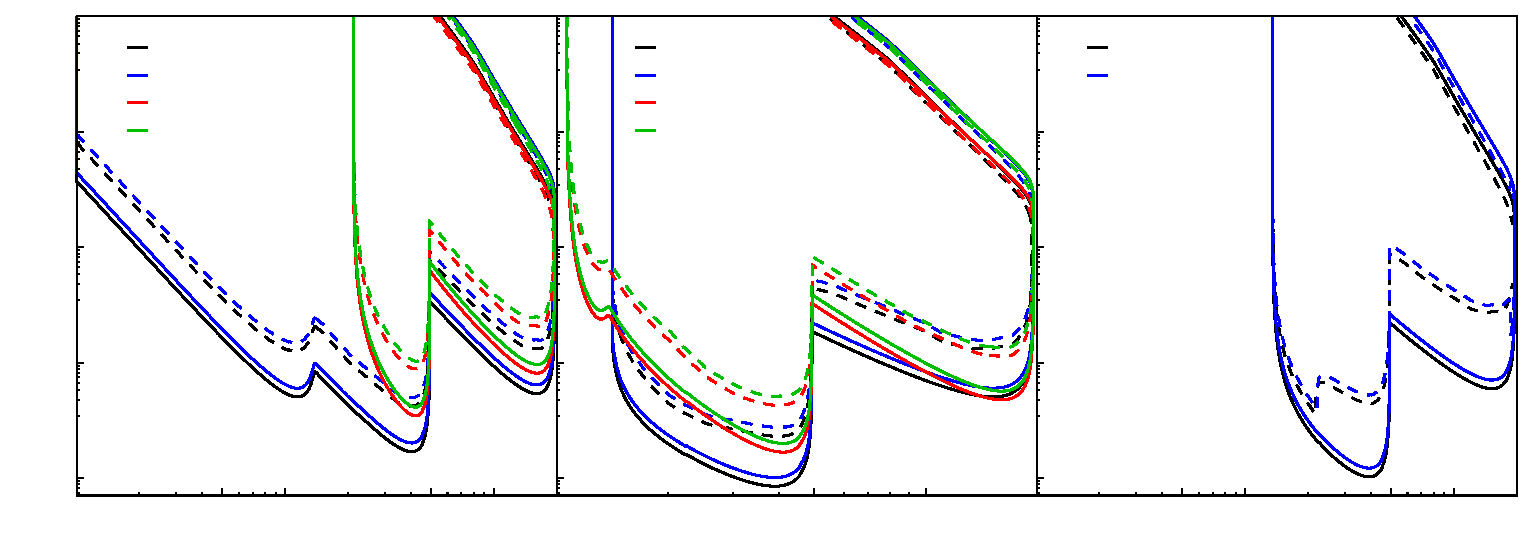
\includegraphics{pics/sensmulti_EW2_real}}%
    \gplfronttext
  \end{picture}%
\endgroup
}}
	\vspace{0.05em}

	%{\resizebox{\linewidth}{!}{\input{pics/sensmulti_MW.tex}}}
	{\resizebox{\linewidth}{!}{% GNUPLOT: LaTeX picture with Postscript
\begingroup
  \makeatletter
  \providecommand\color[2][]{%
    \GenericError{(gnuplot) \space\space\space\@spaces}{%
      Package color not loaded in conjunction with
      terminal option `colourtext'%
    }{See the gnuplot documentation for explanation.%
    }{Either use 'blacktext' in gnuplot or load the package
      color.sty in LaTeX.}%
    \renewcommand\color[2][]{}%
  }%
  \providecommand\includegraphics[2][]{%
    \GenericError{(gnuplot) \space\space\space\@spaces}{%
      Package graphicx or graphics not loaded%
    }{See the gnuplot documentation for explanation.%
    }{The gnuplot epslatex terminal needs graphicx.sty or graphics.sty.}%
    \renewcommand\includegraphics[2][]{}%
  }%
  \providecommand\rotatebox[2]{#2}%
  \@ifundefined{ifGPcolor}{%
    \newif\ifGPcolor
    \GPcolortrue
  }{}%
  \@ifundefined{ifGPblacktext}{%
    \newif\ifGPblacktext
    \GPblacktexttrue
  }{}%
  % define a \g@addto@macro without @ in the name:
  \let\gplgaddtomacro\g@addto@macro
  % define empty templates for all commands taking text:
  \gdef\gplbacktext{}%
  \gdef\gplfronttext{}%
  \makeatother
  \ifGPblacktext
    % no textcolor at all
    \def\colorrgb#1{}%
    \def\colorgray#1{}%
  \else
    % gray or color?
    \ifGPcolor
      \def\colorrgb#1{\color[rgb]{#1}}%
      \def\colorgray#1{\color[gray]{#1}}%
      \expandafter\def\csname LTw\endcsname{\color{white}}%
      \expandafter\def\csname LTb\endcsname{\color{black}}%
      \expandafter\def\csname LTa\endcsname{\color{black}}%
      \expandafter\def\csname LT0\endcsname{\color[rgb]{1,0,0}}%
      \expandafter\def\csname LT1\endcsname{\color[rgb]{0,1,0}}%
      \expandafter\def\csname LT2\endcsname{\color[rgb]{0,0,1}}%
      \expandafter\def\csname LT3\endcsname{\color[rgb]{1,0,1}}%
      \expandafter\def\csname LT4\endcsname{\color[rgb]{0,1,1}}%
      \expandafter\def\csname LT5\endcsname{\color[rgb]{1,1,0}}%
      \expandafter\def\csname LT6\endcsname{\color[rgb]{0,0,0}}%
      \expandafter\def\csname LT7\endcsname{\color[rgb]{1,0.3,0}}%
      \expandafter\def\csname LT8\endcsname{\color[rgb]{0.5,0.5,0.5}}%
    \else
      % gray
      \def\colorrgb#1{\color{black}}%
      \def\colorgray#1{\color[gray]{#1}}%
      \expandafter\def\csname LTw\endcsname{\color{white}}%
      \expandafter\def\csname LTb\endcsname{\color{black}}%
      \expandafter\def\csname LTa\endcsname{\color{black}}%
      \expandafter\def\csname LT0\endcsname{\color{black}}%
      \expandafter\def\csname LT1\endcsname{\color{black}}%
      \expandafter\def\csname LT2\endcsname{\color{black}}%
      \expandafter\def\csname LT3\endcsname{\color{black}}%
      \expandafter\def\csname LT4\endcsname{\color{black}}%
      \expandafter\def\csname LT5\endcsname{\color{black}}%
      \expandafter\def\csname LT6\endcsname{\color{black}}%
      \expandafter\def\csname LT7\endcsname{\color{black}}%
      \expandafter\def\csname LT8\endcsname{\color{black}}%
    \fi
  \fi
    \setlength{\unitlength}{0.0500bp}%
    \ifx\gptboxheight\undefined%
      \newlength{\gptboxheight}%
      \newlength{\gptboxwidth}%
      \newsavebox{\gptboxtext}%
    \fi%
    \setlength{\fboxrule}{0.5pt}%
    \setlength{\fboxsep}{1pt}%
\begin{picture}(14400.00,5040.00)%
    \gplgaddtomacro\gplbacktext{%
      \csname LTb\endcsname%%
      \put(444,607){\makebox(0,0)[r]{\strut{}\np{e-10}}}%
      \put(444,1715){\makebox(0,0)[r]{\strut{}\np{e-8}}}%
      \put(444,2823){\makebox(0,0)[r]{\strut{}\np{e-6}}}%
      \put(444,3931){\makebox(0,0)[r]{\strut{}\np{e-4}}}%
      \put(444,5039){\makebox(0,0)[r]{\strut{}\np{e-2}}}%
      \put(1975,220){\makebox(0,0){\strut{}$0.05$}}%
      \put(3978,220){\makebox(0,0){\strut{}$0.5$}}%
      \put(576,220){\makebox(0,0){\strut{}$0.01$}}%
      \put(2578,220){\makebox(0,0){\strut{}$0.1$}}%
      \put(4580,220){\makebox(0,0){\strut{}$1$}}%
    }%
    \gplgaddtomacro\gplfronttext{%
      \csname LTb\endcsname%%
      \put(-436,2739){\rotatebox{-270}{\makebox(0,0){\strut{}$ |U_{\mu N}|^2 $}}}%
      \put(2879,-110){\makebox(0,0){\strut{}Mass (GeV)}}%
      \csname LTb\endcsname%%
      \put(1388,1583){\makebox(0,0)[l]{\strut{}$\nu e e $ Majorana}}%
      \csname LTb\endcsname%%
      \put(1388,1319){\makebox(0,0)[l]{\strut{}$\nu e e $ Dirac}}%
      \csname LTb\endcsname%%
      \put(1388,1055){\makebox(0,0)[l]{\strut{}$\nu \mu \mu $ Majorana}}%
      \csname LTb\endcsname%%
      \put(1388,791){\makebox(0,0)[l]{\strut{}$\nu \mu \mu $ Dirac}}%
    }%
    \gplgaddtomacro\gplbacktext{%
      \csname LTb\endcsname%%
      \put(5052,607){\makebox(0,0)[r]{\strut{}}}%
      \put(5052,1715){\makebox(0,0)[r]{\strut{}}}%
      \put(5052,2823){\makebox(0,0)[r]{\strut{}}}%
      \put(5052,3931){\makebox(0,0)[r]{\strut{}}}%
      \put(5052,5039){\makebox(0,0)[r]{\strut{}}}%
      \put(7659,220){\makebox(0,0){\strut{}$0.5$}}%
      \put(5184,220){\makebox(0,0){\strut{}$0.1$}}%
      \put(8725,220){\makebox(0,0){\strut{}$1$}}%
    }%
    \gplgaddtomacro\gplfronttext{%
      \csname LTb\endcsname%%
      \put(7487,-110){\makebox(0,0){\strut{}Mass (GeV)}}%
      \csname LTb\endcsname%%
      \put(8118,1583){\makebox(0,0)[l]{\strut{}$\mu \pi $ Majorana}}%
      \csname LTb\endcsname%%
      \put(8118,1319){\makebox(0,0)[l]{\strut{}$\mu \pi $ Dirac}}%
      \csname LTb\endcsname%%
      \put(8118,1055){\makebox(0,0)[l]{\strut{}$\nu e \mu $ Majorana}}%
      \csname LTb\endcsname%%
      \put(8118,791){\makebox(0,0)[l]{\strut{}$\nu e \mu $ Dirac}}%
    }%
    \gplgaddtomacro\gplbacktext{%
      \csname LTb\endcsname%%
      \put(9660,607){\makebox(0,0)[r]{\strut{}}}%
      \put(9660,1715){\makebox(0,0)[r]{\strut{}}}%
      \put(9660,2823){\makebox(0,0)[r]{\strut{}}}%
      \put(9660,3931){\makebox(0,0)[r]{\strut{}}}%
      \put(9660,5039){\makebox(0,0)[r]{\strut{}}}%
      \put(11191,220){\makebox(0,0){\strut{}$0.05$}}%
      \put(13194,220){\makebox(0,0){\strut{}$0.5$}}%
      \put(14399,220){\makebox(0,0){\strut{}$2$}}%
      \put(9792,220){\makebox(0,0){\strut{}$0.01$}}%
      \put(11794,220){\makebox(0,0){\strut{}$0.1$}}%
      \put(13796,220){\makebox(0,0){\strut{}$1$}}%
    }%
    \gplgaddtomacro\gplfronttext{%
      \csname LTb\endcsname%%
      \put(12095,-110){\makebox(0,0){\strut{}Mass (GeV)}}%
      \csname LTb\endcsname%%
      \put(10604,1583){\makebox(0,0)[l]{\strut{}$\nu \pi^0 $ Majorana}}%
      \csname LTb\endcsname%%
      \put(10604,1319){\makebox(0,0)[l]{\strut{}$\nu \pi^0 $ Dirac}}%
    }%
    \gplbacktext
    \put(0,0){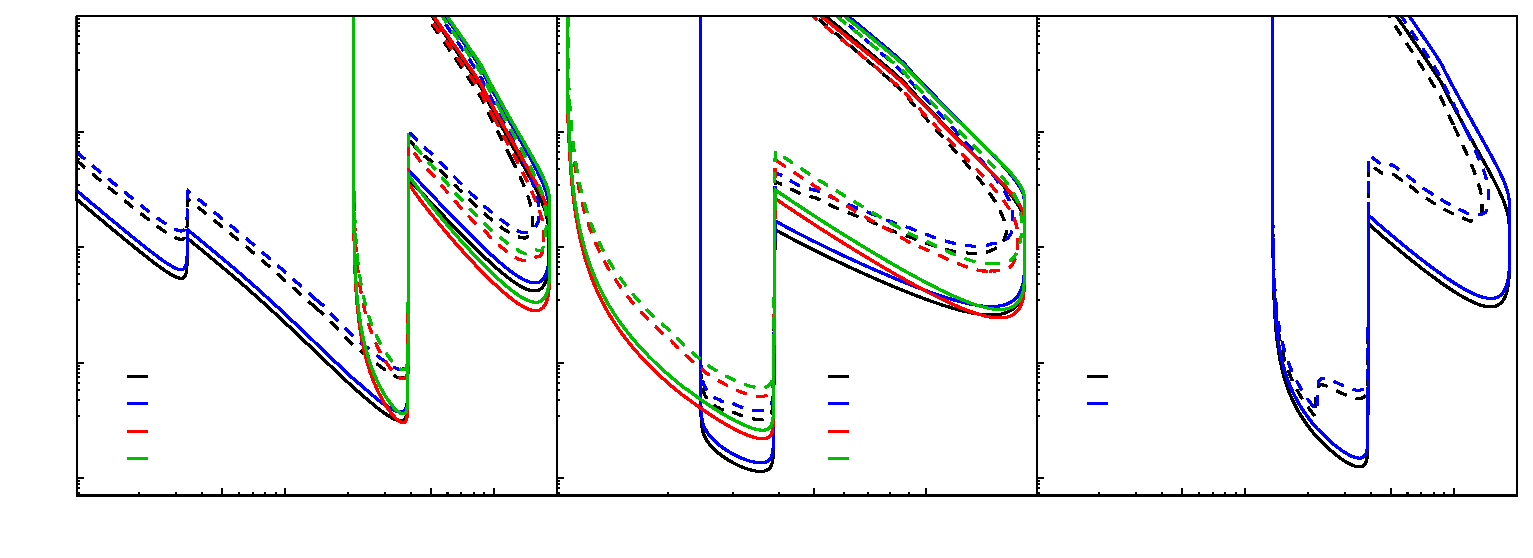
\includegraphics{pics/sensmulti_MW2_real}}%
    \gplfronttext
  \end{picture}%
\endgroup
}}
	\vspace{0.05em}

	%{\resizebox{\linewidth}{!}{\input{pics/sensmulti_TW.tex}}}
	{\resizebox{\linewidth}{!}{% GNUPLOT: LaTeX picture with Postscript
\begingroup
  \makeatletter
  \providecommand\color[2][]{%
    \GenericError{(gnuplot) \space\space\space\@spaces}{%
      Package color not loaded in conjunction with
      terminal option `colourtext'%
    }{See the gnuplot documentation for explanation.%
    }{Either use 'blacktext' in gnuplot or load the package
      color.sty in LaTeX.}%
    \renewcommand\color[2][]{}%
  }%
  \providecommand\includegraphics[2][]{%
    \GenericError{(gnuplot) \space\space\space\@spaces}{%
      Package graphicx or graphics not loaded%
    }{See the gnuplot documentation for explanation.%
    }{The gnuplot epslatex terminal needs graphicx.sty or graphics.sty.}%
    \renewcommand\includegraphics[2][]{}%
  }%
  \providecommand\rotatebox[2]{#2}%
  \@ifundefined{ifGPcolor}{%
    \newif\ifGPcolor
    \GPcolortrue
  }{}%
  \@ifundefined{ifGPblacktext}{%
    \newif\ifGPblacktext
    \GPblacktexttrue
  }{}%
  % define a \g@addto@macro without @ in the name:
  \let\gplgaddtomacro\g@addto@macro
  % define empty templates for all commands taking text:
  \gdef\gplbacktext{}%
  \gdef\gplfronttext{}%
  \makeatother
  \ifGPblacktext
    % no textcolor at all
    \def\colorrgb#1{}%
    \def\colorgray#1{}%
  \else
    % gray or color?
    \ifGPcolor
      \def\colorrgb#1{\color[rgb]{#1}}%
      \def\colorgray#1{\color[gray]{#1}}%
      \expandafter\def\csname LTw\endcsname{\color{white}}%
      \expandafter\def\csname LTb\endcsname{\color{black}}%
      \expandafter\def\csname LTa\endcsname{\color{black}}%
      \expandafter\def\csname LT0\endcsname{\color[rgb]{1,0,0}}%
      \expandafter\def\csname LT1\endcsname{\color[rgb]{0,1,0}}%
      \expandafter\def\csname LT2\endcsname{\color[rgb]{0,0,1}}%
      \expandafter\def\csname LT3\endcsname{\color[rgb]{1,0,1}}%
      \expandafter\def\csname LT4\endcsname{\color[rgb]{0,1,1}}%
      \expandafter\def\csname LT5\endcsname{\color[rgb]{1,1,0}}%
      \expandafter\def\csname LT6\endcsname{\color[rgb]{0,0,0}}%
      \expandafter\def\csname LT7\endcsname{\color[rgb]{1,0.3,0}}%
      \expandafter\def\csname LT8\endcsname{\color[rgb]{0.5,0.5,0.5}}%
    \else
      % gray
      \def\colorrgb#1{\color{black}}%
      \def\colorgray#1{\color[gray]{#1}}%
      \expandafter\def\csname LTw\endcsname{\color{white}}%
      \expandafter\def\csname LTb\endcsname{\color{black}}%
      \expandafter\def\csname LTa\endcsname{\color{black}}%
      \expandafter\def\csname LT0\endcsname{\color{black}}%
      \expandafter\def\csname LT1\endcsname{\color{black}}%
      \expandafter\def\csname LT2\endcsname{\color{black}}%
      \expandafter\def\csname LT3\endcsname{\color{black}}%
      \expandafter\def\csname LT4\endcsname{\color{black}}%
      \expandafter\def\csname LT5\endcsname{\color{black}}%
      \expandafter\def\csname LT6\endcsname{\color{black}}%
      \expandafter\def\csname LT7\endcsname{\color{black}}%
      \expandafter\def\csname LT8\endcsname{\color{black}}%
    \fi
  \fi
    \setlength{\unitlength}{0.0500bp}%
    \ifx\gptboxheight\undefined%
      \newlength{\gptboxheight}%
      \newlength{\gptboxwidth}%
      \newsavebox{\gptboxtext}%
    \fi%
    \setlength{\fboxrule}{0.5pt}%
    \setlength{\fboxsep}{1pt}%
\begin{picture}(14400.00,5040.00)%
    \gplgaddtomacro\gplbacktext{%
      \csname LTb\endcsname%%
      \put(2748,1097){\makebox(0,0)[r]{\strut{}\np{e-6}}}%
      \put(2748,2411){\makebox(0,0)[r]{\strut{}\np{e-4}}}%
      \put(2748,3725){\makebox(0,0)[r]{\strut{}\np{e-2}}}%
      \put(2748,5039){\makebox(0,0)[r]{\strut{}\np{1}}}%
      \put(4279,220){\makebox(0,0){\strut{}$0.05$}}%
      \put(6282,220){\makebox(0,0){\strut{}$0.5$}}%
      \put(2880,220){\makebox(0,0){\strut{}$0.01$}}%
      \put(4882,220){\makebox(0,0){\strut{}$0.1$}}%
      \put(6884,220){\makebox(0,0){\strut{}$1$}}%
    }%
    \gplgaddtomacro\gplfronttext{%
      \csname LTb\endcsname%%
      \put(2000,2739){\rotatebox{-270}{\makebox(0,0){\strut{}$ |U_{\tau N}|^2 $}}}%
      \put(5183,-110){\makebox(0,0){\strut{}Mass (GeV)}}%
      \csname LTb\endcsname%%
      \put(3692,2081){\makebox(0,0)[l]{\strut{}$\nu e e $ Majorana}}%
      \csname LTb\endcsname%%
      \put(3692,1817){\makebox(0,0)[l]{\strut{}$\nu e e $ Dirac}}%
      \csname LTb\endcsname%%
      \put(3692,1553){\makebox(0,0)[l]{\strut{}$\nu \mu \mu $ Majorana}}%
      \csname LTb\endcsname%%
      \put(3692,1289){\makebox(0,0)[l]{\strut{}$\nu \mu \mu $ Dirac}}%
    }%
    \gplgaddtomacro\gplbacktext{%
      \csname LTb\endcsname%%
      \put(7355,1097){\makebox(0,0)[r]{\strut{}}}%
      \put(7355,2411){\makebox(0,0)[r]{\strut{}}}%
      \put(7355,3725){\makebox(0,0)[r]{\strut{}}}%
      \put(7355,5039){\makebox(0,0)[r]{\strut{}}}%
      \put(8887,220){\makebox(0,0){\strut{}$0.05$}}%
      \put(10889,220){\makebox(0,0){\strut{}$0.5$}}%
      \put(12095,220){\makebox(0,0){\strut{}$2$}}%
      \put(7487,220){\makebox(0,0){\strut{}$0.01$}}%
      \put(9490,220){\makebox(0,0){\strut{}$0.1$}}%
      \put(11492,220){\makebox(0,0){\strut{}$1$}}%
    }%
    \gplgaddtomacro\gplfronttext{%
      \csname LTb\endcsname%%
      \put(9791,-110){\makebox(0,0){\strut{}Mass (GeV)}}%
      \csname LTb\endcsname%%
      \put(8299,2081){\makebox(0,0)[l]{\strut{}$\nu \pi^0 $ Majorana}}%
      \csname LTb\endcsname%%
      \put(8299,1817){\makebox(0,0)[l]{\strut{}$\nu \pi^0 $ Dirac}}%
    }%
    \gplbacktext
    \put(0,0){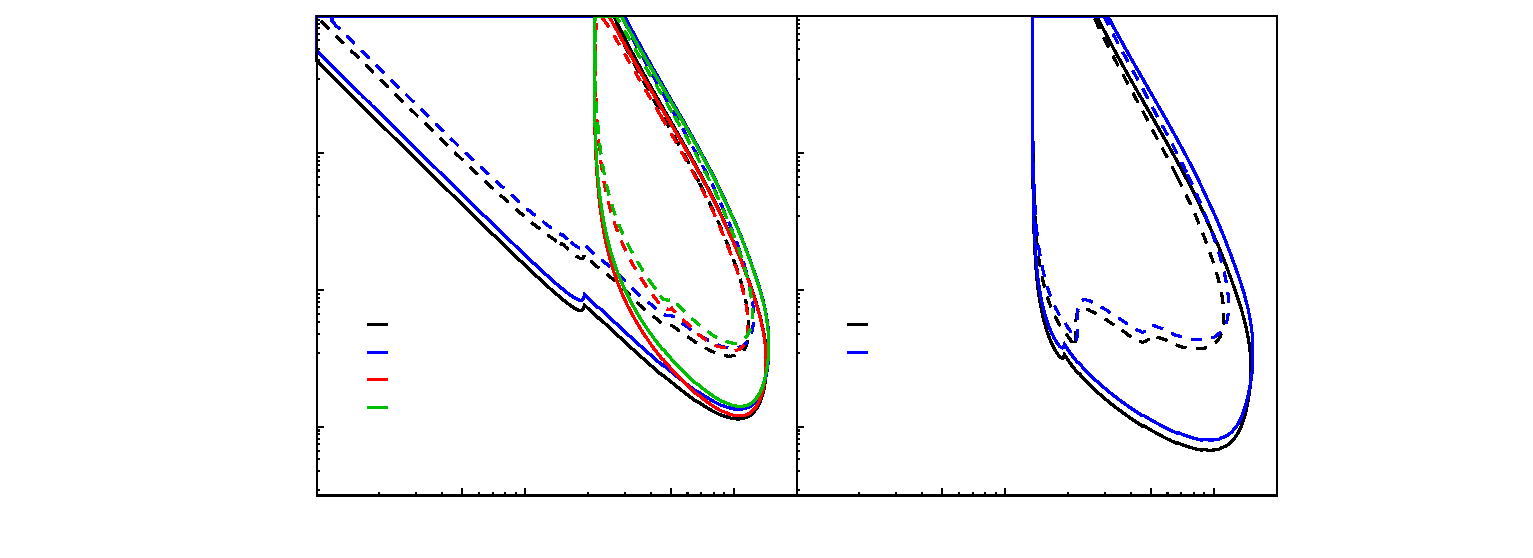
\includegraphics{pics/sensmulti_TW2_real}}%
    \gplfronttext
  \end{picture}%
\endgroup
}}

	\caption[Sensitivity regions to individual channels for dominant mixings with background analysis]%
		{The 90\,\% C.L. sensitivity regions to individual channels for dominant mixings %
		$|U_{e N}|^2$ (top), $|U_{\mu N}|^2$ (middle), and $|U_{\tau N}|^2$ (bottom) are shown.
		The solid lines correspond to the analysis before the background analysis, which is equivalent %
		to a weighting factor $W_d = 1$ (see~\refeq{eq:event}).
		The dashed lines are drawn after the background analysis.
		The distinction between the fermionic natures are explained in the colour key.}
	\label{fig:senseW}
\end{figure}


\begin{table}
	\centering
	\caption[Results from single dominant mixing]%
		{This table summarises the sensitivity result for single dominant mixing and for each decay channel.
			The minimum value of the mixing to Majorana HNLs to which DUNE ND is sensitive to is reported; %
			the value in bracket is with the background analysis included.
		}
	\label{tab:main_result}
	\small
	\begin{tabular}{lccc}
		\toprule
		Channel	& $|U_{e N}|^2$ & $|U_{\mu N}|^2$ & $|U_{\tau N}|^2$ 	\\
		\midrule
		$N\to\nu e^+ e^-$	& \np{2.9e-10} (\np{24.5e-10})	& \np{9.9e-10} (\np{73.1e-10})	& \np{1.3e-6} (\np{17.6e-6})	\\
		$N\to\nu e^\pm \mu^\mp$	& \np{2.3e-10} (\np{5.1e-10})	& \np{4.8e-10} (\np{6.4e-10})	& --	\\
		$N\to\nu \mu^+ \mu^-$	& \np{12.0e-10} (\np{46.5e-10})	& \np{9.2e-10} (\np{16.6e-10})	& \np{1.5e-6} (\np{40.0e-6})	\\
		$N\to\nu \pi^0$		& \np{1.1e-10} (\np{29.8e-10})	& \np{1.5e-10} (\np{36.9e-10})	& \np{4.6e-7} (\np{2.21e-5})	\\
		$N\to e^\mp \pi^\pm$	& \np{0.7e-10} (\np{4.3e-10})	& --				& --	\\
		$N\to\mu^\mp \pi^\pm$	& --				& \np{1.3e-10} (\np{19.9e-10})	& --	\\
		\bottomrule
	\end{tabular}
\end{table}

The sensitivity regions for the three mixings $|U_{e N}|^2$, $|U_{\mu N}|^2$, and %
$|U_{\tau N}|^2$ are presented here with the assumption that just one mixing element dominates over the other two.
The~sensitivities for the decay channels $N\to\nu e^+ e^-$, $\nu e^\pm \mu^\mp$, $\nu \mu^+ \mu^-$, $\nu \pi^0$, % 
$e^\mp \pi^\pm$ ($|U_{e N}|^2$ only), and $\mu^\mp \pi^\pm$ ($|U_{\mu N}|^2$ only) are reported in \reffig{fig:senseW}.
The solid lines corresponds to a scenario in which zero background is assumed at the ND.
%The introduction of background worsens the sensitives, the lines of which are represented by dashed lines.
A background evaluation was carried out for these channels (see~\refsec{sec:background}), %
in order to define a more realistic sensitivity; %
the resulting regions are shown as dashed lines in \reffig{fig:senseW}.
The final sensitivity will lie somewhere between the lines with and without backgrounds,
since it is expected that further improvements to background reduction can be achieved %
with a dedicated analysis by the experimental collaboration, %

For both the electronic and the muonic mixings, the two-body semileptonic decay modes are the ones providing %
the best sensitivity for sufficiently heavy masses.
With the channel $N\to e^\mp \pi^\pm$, the mixing can be constrained in the range %
$0.15\,\text{GeV} \lesssim m_N \lesssim 0.49\,\text{GeV}$ %
to be $|U_{e N}|^2 < \np{3e-9}$, with a minimum point $|U_{e N}|^2 < \np{7e-11}$ at $m_N \simeq 0.39$\,GeV.
Including the background rejection, the limits are loosened by a factor of $\sim6.1$.
The~channel $N\to \mu^\mp \pi^\pm$ can constrain the mixing $|U_{\mu N}|^2 < \np{5.6e-10}$ %
in the mass range \mbox{$0.25\,\text{GeV} \lesssim m_N \lesssim 0.39\,\text{GeV}$}, %
with the best limit $|U_{\mu N}|^2 < \np{1.3e-10}$ at $m_N \simeq 0.35$\,GeV.
In this case, the higher background reduce the bounds up to a factor of $\sim15.1$.
The NC decay $N\to \nu \pi^0$ is the channel most affected by background and with the worst signal efficiency: %
the limits are higher at most by a factor of~$\sim$27.1 for the electronic, %
$\sim$24.6 for the muonic, and~$\sim$52.6 for the tau mixing.
Assuming no background, instead, the constrains placed by this decay mode can be competitive, as the %
mixings are limited to be $|U_{e N}|^2 < \np{1.1e-10}$ at $m_N \simeq 0.39$\,GeV, %
$|U_{\mu N}|^2 < \np{1.5e-10}$ at $m_N \simeq 0.35$\,GeV, %
and $|U_{\tau N}|^2 < \np{4.6e-7}$ at $m_N \simeq 0.95$\,GeV.
%This difference is due to the fact that charge-ID is not taken in account in our analysis.
There is no sensitivity to the channel $N\to\tau^\mp\pi^\pm$ because of the subdominant branching ratio %
and flux content.

The three-body lepton decays have a lower reach, but are more sensitive to masses above the kaon mass limit %
than the two-body semileptonic modes.
The channel $N\to \nu e^- e^+$ is the only one that covers the whole mass range of interest %
and the bounds are weakened by background reduction by a factor less than 8 for mixings with electron and muon flavours.
It can limit the electronic mixing down to $|U_{e N}|^2 < \np{2.5e-9}$ at $m_N \simeq 0.11$\,GeV, %
$|U_{e N}|^2 < \np{2.9e-10}$ at $m_N \simeq 0.39$\,GeV, and $|U_{e N}|^2 < \np{3.0e-9}$ at $m_N \simeq 1.6$\,GeV.
The channels $N \to\nu \mu^- \mu^+$ and $\nu e^\pm \mu^\mp$ perform better with the muon mixing %
for which the residual background is very little, as one muon and one electron or two muons are required in the final state.
The bounds are weakened at most by a factor of $\sim1.8$ for the muon mixing.
These two channels respectively give the limits %
$|U_{\mu N}|^2 < \np{9.9e-10}$ at $m_N \simeq 0.37$\,GeV and $|U_{\mu N}|^2 < \np{8.0e-8}$ at $m_N \simeq 1.6$\,GeV, and %
$|U_{\mu N}|^2 < \np{4.8e-10}$ at $m_N \simeq 0.36$\,GeV and $|U_{\mu N}|^2 < \np{5.6e-8}$ at $m_N \simeq 1.6$\,GeV.
The $\tau$ sector can only be constrained by the two NC--mediated channels, %
which give very similar constraints near $m_N\simeq 1.0$\,GeV, these being $|U_{\tau N}|^2 < \np{1.3e-6}$ 
for the $\nu e^- e^+$ channel and $|U_{\tau N}|^2 < \np{1.5e-6}$ for the $\nu \mu^- \mu ^+$ channel.

%These regions are naturally weakened when the background analysis is taken in account.
%Instead of performing an event simulation for each value of the heavy neutrino mass, %
%we study the background expectancy only for 9 equally-spaced choices of heavy neutrino mass from 50 MeV to 450 MeV and we interpolate in between.
%%
%	%The weighting factors $W_d$ explained in section~\ref{sec:numevt} are extrapolated in the same manner.
%The channels less afflicted from background reduction analysis are the decays $N\to \ell_\alpha^- \pi^+$, %
%$N\to \nu e^-e^+$, and $N\to \nu e^\mp\mu^\pm$, the sensitivities of which are reduced by less than a factor of 10.
%The other channels present more background and the reduction in the sensitivity is slightly more than one order of magnitude.
%No background analysis is made for masses above the kaon mass.

\begin{figure}[t]
	\centering
	%{\resizebox{\linewidth}{!}{\input{pics/sens_EM_V.tex}}}
	{\resizebox{\linewidth}{!}{% GNUPLOT: LaTeX picture with Postscript
\begingroup
  \makeatletter
  \providecommand\color[2][]{%
    \GenericError{(gnuplot) \space\space\space\@spaces}{%
      Package color not loaded in conjunction with
      terminal option `colourtext'%
    }{See the gnuplot documentation for explanation.%
    }{Either use 'blacktext' in gnuplot or load the package
      color.sty in LaTeX.}%
    \renewcommand\color[2][]{}%
  }%
  \providecommand\includegraphics[2][]{%
    \GenericError{(gnuplot) \space\space\space\@spaces}{%
      Package graphicx or graphics not loaded%
    }{See the gnuplot documentation for explanation.%
    }{The gnuplot epslatex terminal needs graphicx.sty or graphics.sty.}%
    \renewcommand\includegraphics[2][]{}%
  }%
  \providecommand\rotatebox[2]{#2}%
  \@ifundefined{ifGPcolor}{%
    \newif\ifGPcolor
    \GPcolortrue
  }{}%
  \@ifundefined{ifGPblacktext}{%
    \newif\ifGPblacktext
    \GPblacktexttrue
  }{}%
  % define a \g@addto@macro without @ in the name:
  \let\gplgaddtomacro\g@addto@macro
  % define empty templates for all commands taking text:
  \gdef\gplbacktext{}%
  \gdef\gplfronttext{}%
  \makeatother
  \ifGPblacktext
    % no textcolor at all
    \def\colorrgb#1{}%
    \def\colorgray#1{}%
  \else
    % gray or color?
    \ifGPcolor
      \def\colorrgb#1{\color[rgb]{#1}}%
      \def\colorgray#1{\color[gray]{#1}}%
      \expandafter\def\csname LTw\endcsname{\color{white}}%
      \expandafter\def\csname LTb\endcsname{\color{black}}%
      \expandafter\def\csname LTa\endcsname{\color{black}}%
      \expandafter\def\csname LT0\endcsname{\color[rgb]{1,0,0}}%
      \expandafter\def\csname LT1\endcsname{\color[rgb]{0,1,0}}%
      \expandafter\def\csname LT2\endcsname{\color[rgb]{0,0,1}}%
      \expandafter\def\csname LT3\endcsname{\color[rgb]{1,0,1}}%
      \expandafter\def\csname LT4\endcsname{\color[rgb]{0,1,1}}%
      \expandafter\def\csname LT5\endcsname{\color[rgb]{1,1,0}}%
      \expandafter\def\csname LT6\endcsname{\color[rgb]{0,0,0}}%
      \expandafter\def\csname LT7\endcsname{\color[rgb]{1,0.3,0}}%
      \expandafter\def\csname LT8\endcsname{\color[rgb]{0.5,0.5,0.5}}%
    \else
      % gray
      \def\colorrgb#1{\color{black}}%
      \def\colorgray#1{\color[gray]{#1}}%
      \expandafter\def\csname LTw\endcsname{\color{white}}%
      \expandafter\def\csname LTb\endcsname{\color{black}}%
      \expandafter\def\csname LTa\endcsname{\color{black}}%
      \expandafter\def\csname LT0\endcsname{\color{black}}%
      \expandafter\def\csname LT1\endcsname{\color{black}}%
      \expandafter\def\csname LT2\endcsname{\color{black}}%
      \expandafter\def\csname LT3\endcsname{\color{black}}%
      \expandafter\def\csname LT4\endcsname{\color{black}}%
      \expandafter\def\csname LT5\endcsname{\color{black}}%
      \expandafter\def\csname LT6\endcsname{\color{black}}%
      \expandafter\def\csname LT7\endcsname{\color{black}}%
      \expandafter\def\csname LT8\endcsname{\color{black}}%
    \fi
  \fi
    \setlength{\unitlength}{0.0500bp}%
    \ifx\gptboxheight\undefined%
      \newlength{\gptboxheight}%
      \newlength{\gptboxwidth}%
      \newsavebox{\gptboxtext}%
    \fi%
    \setlength{\fboxrule}{0.5pt}%
    \setlength{\fboxsep}{1pt}%
\begin{picture}(14400.00,5040.00)%
    \gplgaddtomacro\gplbacktext{%
      \csname LTb\endcsname%%
      \put(444,951){\makebox(0,0)[r]{\strut{}\np{e-8}}}%
      \put(444,1973){\makebox(0,0)[r]{\strut{}\np{e-6}}}%
      \put(444,2995){\makebox(0,0)[r]{\strut{}\np{e-4}}}%
      \put(444,4017){\makebox(0,0)[r]{\strut{}\np{e-2}}}%
      \put(444,5039){\makebox(0,0)[r]{\strut{}\np{e0}}}%
      \put(1015,220){\makebox(0,0){\strut{}$0.5$}}%
      \put(2379,220){\makebox(0,0){\strut{}$1$}}%
    }%
    \gplgaddtomacro\gplfronttext{%
      \csname LTb\endcsname%%
      \put(-304,2739){\rotatebox{-270}{\makebox(0,0){\strut{}$ |U_{e N}|^2 $}}}%
      \put(2159,-110){\makebox(0,0){\strut{}Mass (GeV)}}%
      \csname LTb\endcsname%%
      \put(2838,4753){\makebox(0,0)[l]{\strut{}$e K$}}%
      \csname LTb\endcsname%%
      \put(2838,4489){\makebox(0,0)[l]{\strut{}$e K^*$}}%
      \csname LTb\endcsname%%
      \put(2838,4225){\makebox(0,0)[l]{\strut{}$e \rho$}}%
      \csname LTb\endcsname%%
      \put(2838,3961){\makebox(0,0)[l]{\strut{}$\nu\rho^0$}}%
    }%
    \gplgaddtomacro\gplbacktext{%
      \csname LTb\endcsname%%
      \put(3611,951){\makebox(0,0)[r]{\strut{}}}%
      \put(3611,1973){\makebox(0,0)[r]{\strut{}}}%
      \put(3611,2995){\makebox(0,0)[r]{\strut{}}}%
      \put(3611,4017){\makebox(0,0)[r]{\strut{}}}%
      \put(3611,5039){\makebox(0,0)[r]{\strut{}}}%
      \put(4182,220){\makebox(0,0){\strut{}$0.5$}}%
      \put(6911,220){\makebox(0,0){\strut{}$2$}}%
      \put(5547,220){\makebox(0,0){\strut{}$1$}}%
    }%
    \gplgaddtomacro\gplfronttext{%
      \csname LTb\endcsname%%
      \put(5327,-110){\makebox(0,0){\strut{}Mass (GeV)}}%
      \csname LTb\endcsname%%
      \put(6006,4753){\makebox(0,0)[l]{\strut{}$\nu\eta$}}%
      \csname LTb\endcsname%%
      \put(6006,4489){\makebox(0,0)[l]{\strut{}$\nu\eta'$}}%
      \csname LTb\endcsname%%
      \put(6006,4225){\makebox(0,0)[l]{\strut{}$\nu\omega$}}%
      \csname LTb\endcsname%%
      \put(6006,3961){\makebox(0,0)[l]{\strut{}$\nu\phi$}}%
    }%
    \gplgaddtomacro\gplbacktext{%
      \csname LTb\endcsname%%
      \put(7932,951){\makebox(0,0)[r]{\strut{}\np{e-8}}}%
      \put(7932,1973){\makebox(0,0)[r]{\strut{}\np{e-6}}}%
      \put(7932,2995){\makebox(0,0)[r]{\strut{}\np{e-4}}}%
      \put(7932,4017){\makebox(0,0)[r]{\strut{}\np{e-2}}}%
      \put(7932,5039){\makebox(0,0)[r]{\strut{}\np{e0}}}%
      \put(8064,220){\makebox(0,0){\strut{}$0.5$}}%
      \put(9648,220){\makebox(0,0){\strut{}$1$}}%
    }%
    \gplgaddtomacro\gplfronttext{%
      \csname LTb\endcsname%%
      \put(7184,2739){\rotatebox{-270}{\makebox(0,0){\strut{}$ |U_{\mu 4}|^2 $}}}%
      \put(9647,-110){\makebox(0,0){\strut{}Mass (GeV)}}%
      \csname LTb\endcsname%%
      \put(10107,4753){\makebox(0,0)[l]{\strut{}$\mu K$}}%
      \csname LTb\endcsname%%
      \put(10107,4489){\makebox(0,0)[l]{\strut{}$\mu K^*$}}%
      \csname LTb\endcsname%%
      \put(10107,4225){\makebox(0,0)[l]{\strut{}$\mu \rho$}}%
      \csname LTb\endcsname%%
      \put(10107,3961){\makebox(0,0)[l]{\strut{}$\nu \rho^0$}}%
    }%
    \gplgaddtomacro\gplbacktext{%
      \csname LTb\endcsname%%
      \put(11100,951){\makebox(0,0)[r]{\strut{}}}%
      \put(11100,1973){\makebox(0,0)[r]{\strut{}}}%
      \put(11100,2995){\makebox(0,0)[r]{\strut{}}}%
      \put(11100,4017){\makebox(0,0)[r]{\strut{}}}%
      \put(11100,5039){\makebox(0,0)[r]{\strut{}}}%
      \put(11232,220){\makebox(0,0){\strut{}$0.5$}}%
      \put(14399,220){\makebox(0,0){\strut{}$2$}}%
      \put(12816,220){\makebox(0,0){\strut{}$1$}}%
    }%
    \gplgaddtomacro\gplfronttext{%
      \csname LTb\endcsname%%
      \put(12815,-110){\makebox(0,0){\strut{}Mass (GeV)}}%
      \csname LTb\endcsname%%
      \put(13275,4753){\makebox(0,0)[l]{\strut{}$\nu\eta$}}%
      \csname LTb\endcsname%%
      \put(13275,4489){\makebox(0,0)[l]{\strut{}$\nu\eta'$}}%
      \csname LTb\endcsname%%
      \put(13275,4225){\makebox(0,0)[l]{\strut{}$\nu\omega$}}%
      \csname LTb\endcsname%%
      \put(13275,3961){\makebox(0,0)[l]{\strut{}$\nu\phi$}}%
    }%
    \gplbacktext
    \put(0,0){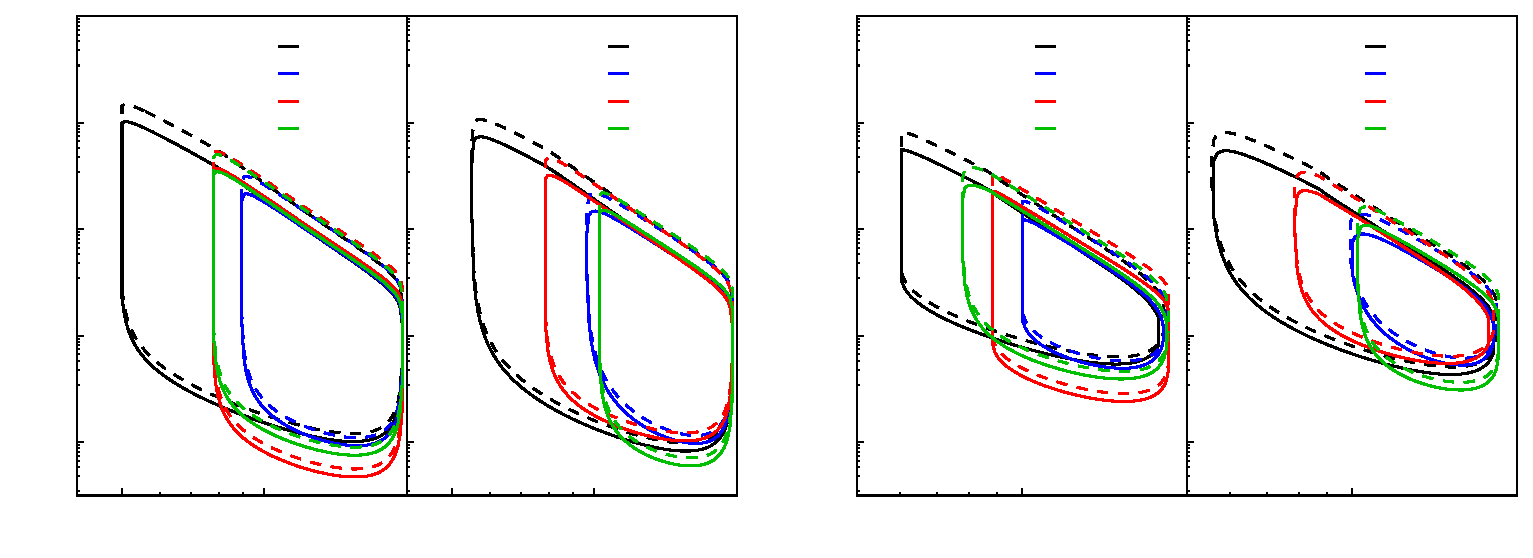
\includegraphics{pics/sensmulti_EM_V2_real}}%
    \gplfronttext
  \end{picture}%
\endgroup
}}
	\vspace{0.05em}

	%{\resizebox{\linewidth}{!}{\input{pics/sens_T_V.tex}}}
	{\resizebox{\linewidth}{!}{% GNUPLOT: LaTeX picture with Postscript
\begingroup
  \makeatletter
  \providecommand\color[2][]{%
    \GenericError{(gnuplot) \space\space\space\@spaces}{%
      Package color not loaded in conjunction with
      terminal option `colourtext'%
    }{See the gnuplot documentation for explanation.%
    }{Either use 'blacktext' in gnuplot or load the package
      color.sty in LaTeX.}%
    \renewcommand\color[2][]{}%
  }%
  \providecommand\includegraphics[2][]{%
    \GenericError{(gnuplot) \space\space\space\@spaces}{%
      Package graphicx or graphics not loaded%
    }{See the gnuplot documentation for explanation.%
    }{The gnuplot epslatex terminal needs graphicx.sty or graphics.sty.}%
    \renewcommand\includegraphics[2][]{}%
  }%
  \providecommand\rotatebox[2]{#2}%
  \@ifundefined{ifGPcolor}{%
    \newif\ifGPcolor
    \GPcolortrue
  }{}%
  \@ifundefined{ifGPblacktext}{%
    \newif\ifGPblacktext
    \GPblacktexttrue
  }{}%
  % define a \g@addto@macro without @ in the name:
  \let\gplgaddtomacro\g@addto@macro
  % define empty templates for all commands taking text:
  \gdef\gplbacktext{}%
  \gdef\gplfronttext{}%
  \makeatother
  \ifGPblacktext
    % no textcolor at all
    \def\colorrgb#1{}%
    \def\colorgray#1{}%
  \else
    % gray or color?
    \ifGPcolor
      \def\colorrgb#1{\color[rgb]{#1}}%
      \def\colorgray#1{\color[gray]{#1}}%
      \expandafter\def\csname LTw\endcsname{\color{white}}%
      \expandafter\def\csname LTb\endcsname{\color{black}}%
      \expandafter\def\csname LTa\endcsname{\color{black}}%
      \expandafter\def\csname LT0\endcsname{\color[rgb]{1,0,0}}%
      \expandafter\def\csname LT1\endcsname{\color[rgb]{0,1,0}}%
      \expandafter\def\csname LT2\endcsname{\color[rgb]{0,0,1}}%
      \expandafter\def\csname LT3\endcsname{\color[rgb]{1,0,1}}%
      \expandafter\def\csname LT4\endcsname{\color[rgb]{0,1,1}}%
      \expandafter\def\csname LT5\endcsname{\color[rgb]{1,1,0}}%
      \expandafter\def\csname LT6\endcsname{\color[rgb]{0,0,0}}%
      \expandafter\def\csname LT7\endcsname{\color[rgb]{1,0.3,0}}%
      \expandafter\def\csname LT8\endcsname{\color[rgb]{0.5,0.5,0.5}}%
    \else
      % gray
      \def\colorrgb#1{\color{black}}%
      \def\colorgray#1{\color[gray]{#1}}%
      \expandafter\def\csname LTw\endcsname{\color{white}}%
      \expandafter\def\csname LTb\endcsname{\color{black}}%
      \expandafter\def\csname LTa\endcsname{\color{black}}%
      \expandafter\def\csname LT0\endcsname{\color{black}}%
      \expandafter\def\csname LT1\endcsname{\color{black}}%
      \expandafter\def\csname LT2\endcsname{\color{black}}%
      \expandafter\def\csname LT3\endcsname{\color{black}}%
      \expandafter\def\csname LT4\endcsname{\color{black}}%
      \expandafter\def\csname LT5\endcsname{\color{black}}%
      \expandafter\def\csname LT6\endcsname{\color{black}}%
      \expandafter\def\csname LT7\endcsname{\color{black}}%
      \expandafter\def\csname LT8\endcsname{\color{black}}%
    \fi
  \fi
    \setlength{\unitlength}{0.0500bp}%
    \ifx\gptboxheight\undefined%
      \newlength{\gptboxheight}%
      \newlength{\gptboxwidth}%
      \newsavebox{\gptboxtext}%
    \fi%
    \setlength{\fboxrule}{0.5pt}%
    \setlength{\fboxsep}{1pt}%
\begin{picture}(14400.00,5040.00)%
    \gplgaddtomacro\gplbacktext{%
      \csname LTb\endcsname%%
      \put(4188,1097){\makebox(0,0)[r]{\strut{}\np{e-6}}}%
      \put(4188,2411){\makebox(0,0)[r]{\strut{}\np{e-4}}}%
      \put(4188,3725){\makebox(0,0)[r]{\strut{}\np{e-2}}}%
      \put(4188,5039){\makebox(0,0)[r]{\strut{}\np{1}}}%
      \put(4759,220){\makebox(0,0){\strut{}$0.5$}}%
      \put(6123,220){\makebox(0,0){\strut{}$1$}}%
    }%
    \gplgaddtomacro\gplfronttext{%
      \csname LTb\endcsname%%
      \put(3440,2739){\rotatebox{-270}{\makebox(0,0){\strut{}$ |U_{\tau N}|^2 $}}}%
      \put(5903,-110){\makebox(0,0){\strut{}Mass (GeV)}}%
      \csname LTb\endcsname%%
      \put(6582,4709){\makebox(0,0)[l]{\strut{}$\nu\eta$}}%
      \csname LTb\endcsname%%
      \put(6582,4445){\makebox(0,0)[l]{\strut{}$\nu\eta'$}}%
      \csname LTb\endcsname%%
      \put(6582,4181){\makebox(0,0)[l]{\strut{}$\nu\phi$}}%
    }%
    \gplgaddtomacro\gplbacktext{%
      \csname LTb\endcsname%%
      \put(7355,1097){\makebox(0,0)[r]{\strut{}}}%
      \put(7355,2411){\makebox(0,0)[r]{\strut{}}}%
      \put(7355,3725){\makebox(0,0)[r]{\strut{}}}%
      \put(7355,5039){\makebox(0,0)[r]{\strut{}}}%
      \put(7926,220){\makebox(0,0){\strut{}$0.5$}}%
      \put(10655,220){\makebox(0,0){\strut{}$2$}}%
      \put(9291,220){\makebox(0,0){\strut{}$1$}}%
    }%
    \gplgaddtomacro\gplfronttext{%
      \csname LTb\endcsname%%
      \put(9071,-110){\makebox(0,0){\strut{}Mass (GeV)}}%
      \csname LTb\endcsname%%
      \put(9750,4709){\makebox(0,0)[l]{\strut{}$\nu\omega$}}%
      \csname LTb\endcsname%%
      \put(9750,4445){\makebox(0,0)[l]{\strut{}$\nu\rho^0$}}%
    }%
    \gplbacktext
    \put(0,0){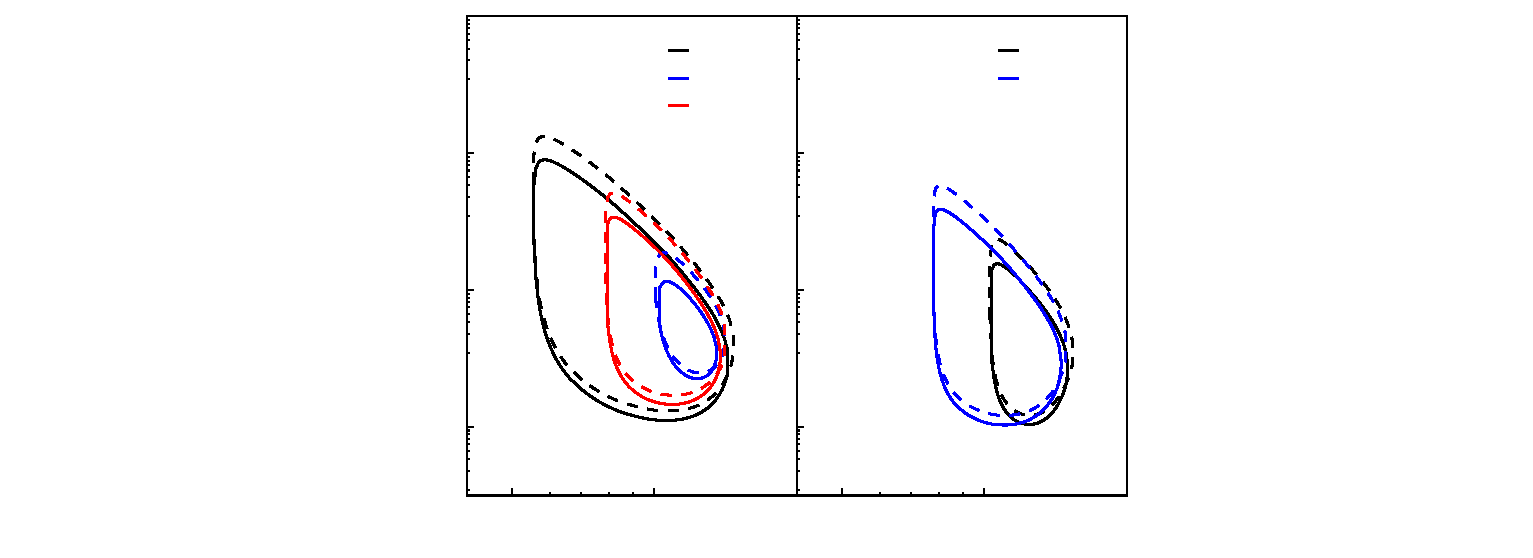
\includegraphics{pics/sensmulti_T_V2_real}}%
    \gplfronttext
  \end{picture}%
\endgroup
}}
	\caption[Sensitivity regions to individual channels for dominant mixings without background analysis]%
		{The 90\,\% C.L. sensitivity regions to individual channels for dominant mixings %
		$|U_{e N}|^2$ (top left), $|U_{\mu N}|^2$ (top right), and $|U_{\mu N}|^2$ (bottom) are presented for Majorana (solid lines) %
		and Dirac (dashed lines) neutrinos.
		No background analysis was performed for the channels shown here (see text).
		These channels become available only for masses above 0.5\,GeV.  }
	\label{fig:senseV}
\end{figure}

A background study was not performed for all the other decay channels, which open up for masses above the $K^0$ mass, %
due to the fact that the final state particles need a more complex analysis.
The sensitivities to these modes are shown in~\reffig{fig:senseV}, and they can place some constraints to the mixing.
All the channels peak in their sensitivity for masses between $1.3$ and $1.8$\,GeV.
The best limits obtained for CC decays are %
$|U_{e N}|^2 < \np{2.3e-9}$ from $N \to e^\mp \rho^\pm$ and $|U_{\mu N}|^2 < \np{6.0e-8}$ from $N \to \mu^\mp \rho^\pm$; %
among the NC decays $|U_{e N}|^2 < \np{3.7e-9}$ and $|U_{\mu N}|^2 < \np{1.0e-7}$ both from $N \to \nu \phi$.
Even for these channels, there is no sensitivity to CC processes to the tau mixing, %
but interesting limits are set from $N\to \nu\eta$, $N\to \nu\omega$, and $\nu\rho^0$ to be respectively %
$|U_{\tau N}|^2 < \np{1.86e-6}$, $\np{3.24e-6}$, and~$\np{1.60e-6}$.

\subsection{Two dominant mixings}
\label{sec:bimax}

\begin{figure}
	\centering
	%{\resizebox{\linewidth}{!}{\input{pics/sens_EM.tex}}}
	{\resizebox{\linewidth}{!}{% GNUPLOT: LaTeX picture with Postscript
\begingroup
  \makeatletter
  \providecommand\color[2][]{%
    \GenericError{(gnuplot) \space\space\space\@spaces}{%
      Package color not loaded in conjunction with
      terminal option `colourtext'%
    }{See the gnuplot documentation for explanation.%
    }{Either use 'blacktext' in gnuplot or load the package
      color.sty in LaTeX.}%
    \renewcommand\color[2][]{}%
  }%
  \providecommand\includegraphics[2][]{%
    \GenericError{(gnuplot) \space\space\space\@spaces}{%
      Package graphicx or graphics not loaded%
    }{See the gnuplot documentation for explanation.%
    }{The gnuplot epslatex terminal needs graphicx.sty or graphics.sty.}%
    \renewcommand\includegraphics[2][]{}%
  }%
  \providecommand\rotatebox[2]{#2}%
  \@ifundefined{ifGPcolor}{%
    \newif\ifGPcolor
    \GPcolortrue
  }{}%
  \@ifundefined{ifGPblacktext}{%
    \newif\ifGPblacktext
    \GPblacktexttrue
  }{}%
  % define a \g@addto@macro without @ in the name:
  \let\gplgaddtomacro\g@addto@macro
  % define empty templates for all commands taking text:
  \gdef\gplbacktext{}%
  \gdef\gplfronttext{}%
  \makeatother
  \ifGPblacktext
    % no textcolor at all
    \def\colorrgb#1{}%
    \def\colorgray#1{}%
  \else
    % gray or color?
    \ifGPcolor
      \def\colorrgb#1{\color[rgb]{#1}}%
      \def\colorgray#1{\color[gray]{#1}}%
      \expandafter\def\csname LTw\endcsname{\color{white}}%
      \expandafter\def\csname LTb\endcsname{\color{black}}%
      \expandafter\def\csname LTa\endcsname{\color{black}}%
      \expandafter\def\csname LT0\endcsname{\color[rgb]{1,0,0}}%
      \expandafter\def\csname LT1\endcsname{\color[rgb]{0,1,0}}%
      \expandafter\def\csname LT2\endcsname{\color[rgb]{0,0,1}}%
      \expandafter\def\csname LT3\endcsname{\color[rgb]{1,0,1}}%
      \expandafter\def\csname LT4\endcsname{\color[rgb]{0,1,1}}%
      \expandafter\def\csname LT5\endcsname{\color[rgb]{1,1,0}}%
      \expandafter\def\csname LT6\endcsname{\color[rgb]{0,0,0}}%
      \expandafter\def\csname LT7\endcsname{\color[rgb]{1,0.3,0}}%
      \expandafter\def\csname LT8\endcsname{\color[rgb]{0.5,0.5,0.5}}%
    \else
      % gray
      \def\colorrgb#1{\color{black}}%
      \def\colorgray#1{\color[gray]{#1}}%
      \expandafter\def\csname LTw\endcsname{\color{white}}%
      \expandafter\def\csname LTb\endcsname{\color{black}}%
      \expandafter\def\csname LTa\endcsname{\color{black}}%
      \expandafter\def\csname LT0\endcsname{\color{black}}%
      \expandafter\def\csname LT1\endcsname{\color{black}}%
      \expandafter\def\csname LT2\endcsname{\color{black}}%
      \expandafter\def\csname LT3\endcsname{\color{black}}%
      \expandafter\def\csname LT4\endcsname{\color{black}}%
      \expandafter\def\csname LT5\endcsname{\color{black}}%
      \expandafter\def\csname LT6\endcsname{\color{black}}%
      \expandafter\def\csname LT7\endcsname{\color{black}}%
      \expandafter\def\csname LT8\endcsname{\color{black}}%
    \fi
  \fi
    \setlength{\unitlength}{0.0500bp}%
    \ifx\gptboxheight\undefined%
      \newlength{\gptboxheight}%
      \newlength{\gptboxwidth}%
      \newsavebox{\gptboxtext}%
    \fi%
    \setlength{\fboxrule}{0.5pt}%
    \setlength{\fboxsep}{1pt}%
\begin{picture}(14400.00,5040.00)%
    \gplgaddtomacro\gplbacktext{%
      \csname LTb\endcsname%%
      \put(444,574){\makebox(0,0)[r]{\strut{}\np{e-10}}}%
      \put(444,1467){\makebox(0,0)[r]{\strut{}\np{e-8}}}%
      \put(444,2360){\makebox(0,0)[r]{\strut{}\np{e-6}}}%
      \put(444,3253){\makebox(0,0)[r]{\strut{}\np{e-4}}}%
      \put(444,4146){\makebox(0,0)[r]{\strut{}\np{e-2}}}%
      \put(444,5039){\makebox(0,0)[r]{\strut{}\np{e0}}}%
      \put(2543,220){\makebox(0,0){\strut{}$0.5$}}%
      \put(816,220){\makebox(0,0){\strut{}$0.1$}}%
      \put(3287,220){\makebox(0,0){\strut{}$1$}}%
    }%
    \gplgaddtomacro\gplfronttext{%
      \csname LTb\endcsname%%
      \put(-436,2739){\rotatebox{-270}{\makebox(0,0){\strut{}$|U_{e N} U_{\mu N}|^2$}}}%
      \put(2303,-110){\makebox(0,0){\strut{}Mass (GeV)}}%
      \csname LTb\endcsname%%
      \put(3503,4864){\makebox(0,0)[l]{\strut{}$\nu e\mu$}}%
      \csname LTb\endcsname%%
      \put(3503,4600){\makebox(0,0)[l]{\strut{}$e\pi$}}%
      \csname LTb\endcsname%%
      \put(3503,4336){\makebox(0,0)[l]{\strut{}$\mu\pi$}}%
      \csname LTb\endcsname%%
      \put(3503,4072){\makebox(0,0)[l]{\strut{}$e K$}}%
      \csname LTb\endcsname%%
      \put(3503,3808){\makebox(0,0)[l]{\strut{}$\mu K$}}%
    }%
    \gplgaddtomacro\gplbacktext{%
      \csname LTb\endcsname%%
      \put(3900,574){\makebox(0,0)[r]{\strut{}}}%
      \put(3900,1467){\makebox(0,0)[r]{\strut{}}}%
      \put(3900,2360){\makebox(0,0)[r]{\strut{}}}%
      \put(3900,3253){\makebox(0,0)[r]{\strut{}}}%
      \put(3900,4146){\makebox(0,0)[r]{\strut{}}}%
      \put(3900,5039){\makebox(0,0)[r]{\strut{}}}%
      \put(5206,220){\makebox(0,0){\strut{}$1$}}%
    }%
    \gplgaddtomacro\gplfronttext{%
      \csname LTb\endcsname%%
      \put(5759,-110){\makebox(0,0){\strut{}Mass (GeV)}}%
      \csname LTb\endcsname%%
      \put(5665,4773){\makebox(0,0)[l]{\strut{}$e\rho$}}%
      \csname LTb\endcsname%%
      \put(5665,4509){\makebox(0,0)[l]{\strut{}$\mu\rho$}}%
      \csname LTb\endcsname%%
      \put(5665,4245){\makebox(0,0)[l]{\strut{}$e K^*$}}%
      \csname LTb\endcsname%%
      \put(5665,3981){\makebox(0,0)[l]{\strut{}$\mu K^*$}}%
    }%
    \gplgaddtomacro\gplbacktext{%
      \csname LTb\endcsname%%
      \put(7355,574){\makebox(0,0)[r]{\strut{}}}%
      \put(7355,1467){\makebox(0,0)[r]{\strut{}}}%
      \put(7355,2360){\makebox(0,0)[r]{\strut{}}}%
      \put(7355,3253){\makebox(0,0)[r]{\strut{}}}%
      \put(7355,4146){\makebox(0,0)[r]{\strut{}}}%
      \put(7355,5039){\makebox(0,0)[r]{\strut{}}}%
      \put(8537,220){\makebox(0,0){\strut{}$0.05$}}%
      \put(10039,220){\makebox(0,0){\strut{}$0.5$}}%
      \put(7487,220){\makebox(0,0){\strut{}$0.01$}}%
      \put(8989,220){\makebox(0,0){\strut{}$0.1$}}%
      \put(10491,220){\makebox(0,0){\strut{}$1$}}%
    }%
    \gplgaddtomacro\gplfronttext{%
      \csname LTb\endcsname%%
      \put(9215,-110){\makebox(0,0){\strut{}Mass (GeV)}}%
      \csname LTb\endcsname%%
      \put(8210,4773){\makebox(0,0)[l]{\strut{}$\nu e e$}}%
      \csname LTb\endcsname%%
      \put(8210,4509){\makebox(0,0)[l]{\strut{}$\nu\mu\mu$}}%
      \csname LTb\endcsname%%
      \put(8210,4245){\makebox(0,0)[l]{\strut{}$\nu\pi^0$}}%
    }%
    \gplgaddtomacro\gplbacktext{%
      \csname LTb\endcsname%%
      \put(10812,574){\makebox(0,0)[r]{\strut{}}}%
      \put(10812,1467){\makebox(0,0)[r]{\strut{}}}%
      \put(10812,2360){\makebox(0,0)[r]{\strut{}}}%
      \put(10812,3253){\makebox(0,0)[r]{\strut{}}}%
      \put(10812,4146){\makebox(0,0)[r]{\strut{}}}%
      \put(10812,5039){\makebox(0,0)[r]{\strut{}}}%
      \put(10944,220){\makebox(0,0){\strut{}$0.5$}}%
      \put(14399,220){\makebox(0,0){\strut{}$2$}}%
      \put(12672,220){\makebox(0,0){\strut{}$1$}}%
    }%
    \gplgaddtomacro\gplfronttext{%
      \csname LTb\endcsname%%
      \put(12671,-110){\makebox(0,0){\strut{}Mass (GeV)}}%
      \csname LTb\endcsname%%
      \put(14003,4773){\makebox(0,0)[l]{\strut{}$\nu\eta$}}%
      \csname LTb\endcsname%%
      \put(14003,4509){\makebox(0,0)[l]{\strut{}$\nu\eta'$}}%
      \csname LTb\endcsname%%
      \put(14003,4245){\makebox(0,0)[l]{\strut{}$\nu\rho^0$}}%
      \csname LTb\endcsname%%
      \put(14003,3981){\makebox(0,0)[l]{\strut{}$\nu\omega$}}%
      \csname LTb\endcsname%%
      \put(14003,3717){\makebox(0,0)[l]{\strut{}$\nu\phi$}}%
    }%
    \gplbacktext
    \put(0,0){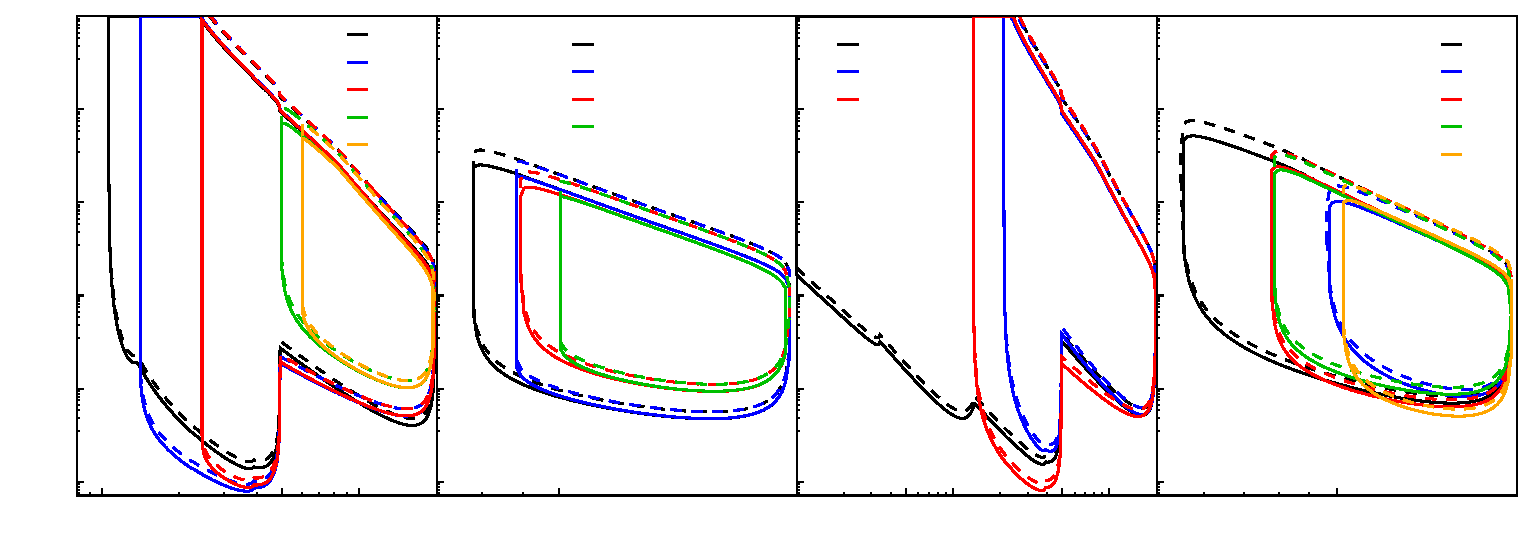
\includegraphics{pics/sensmulti_EM2_real}}%
    \gplfronttext
  \end{picture}%
\endgroup
}}
	\vspace{0.05em}

	%{\resizebox{\linewidth}{!}{\input{pics/sens_MT.tex}}}
	{\resizebox{\linewidth}{!}{% GNUPLOT: LaTeX picture with Postscript
\begingroup
  \makeatletter
  \providecommand\color[2][]{%
    \GenericError{(gnuplot) \space\space\space\@spaces}{%
      Package color not loaded in conjunction with
      terminal option `colourtext'%
    }{See the gnuplot documentation for explanation.%
    }{Either use 'blacktext' in gnuplot or load the package
      color.sty in LaTeX.}%
    \renewcommand\color[2][]{}%
  }%
  \providecommand\includegraphics[2][]{%
    \GenericError{(gnuplot) \space\space\space\@spaces}{%
      Package graphicx or graphics not loaded%
    }{See the gnuplot documentation for explanation.%
    }{The gnuplot epslatex terminal needs graphicx.sty or graphics.sty.}%
    \renewcommand\includegraphics[2][]{}%
  }%
  \providecommand\rotatebox[2]{#2}%
  \@ifundefined{ifGPcolor}{%
    \newif\ifGPcolor
    \GPcolortrue
  }{}%
  \@ifundefined{ifGPblacktext}{%
    \newif\ifGPblacktext
    \GPblacktexttrue
  }{}%
  % define a \g@addto@macro without @ in the name:
  \let\gplgaddtomacro\g@addto@macro
  % define empty templates for all commands taking text:
  \gdef\gplbacktext{}%
  \gdef\gplfronttext{}%
  \makeatother
  \ifGPblacktext
    % no textcolor at all
    \def\colorrgb#1{}%
    \def\colorgray#1{}%
  \else
    % gray or color?
    \ifGPcolor
      \def\colorrgb#1{\color[rgb]{#1}}%
      \def\colorgray#1{\color[gray]{#1}}%
      \expandafter\def\csname LTw\endcsname{\color{white}}%
      \expandafter\def\csname LTb\endcsname{\color{black}}%
      \expandafter\def\csname LTa\endcsname{\color{black}}%
      \expandafter\def\csname LT0\endcsname{\color[rgb]{1,0,0}}%
      \expandafter\def\csname LT1\endcsname{\color[rgb]{0,1,0}}%
      \expandafter\def\csname LT2\endcsname{\color[rgb]{0,0,1}}%
      \expandafter\def\csname LT3\endcsname{\color[rgb]{1,0,1}}%
      \expandafter\def\csname LT4\endcsname{\color[rgb]{0,1,1}}%
      \expandafter\def\csname LT5\endcsname{\color[rgb]{1,1,0}}%
      \expandafter\def\csname LT6\endcsname{\color[rgb]{0,0,0}}%
      \expandafter\def\csname LT7\endcsname{\color[rgb]{1,0.3,0}}%
      \expandafter\def\csname LT8\endcsname{\color[rgb]{0.5,0.5,0.5}}%
    \else
      % gray
      \def\colorrgb#1{\color{black}}%
      \def\colorgray#1{\color[gray]{#1}}%
      \expandafter\def\csname LTw\endcsname{\color{white}}%
      \expandafter\def\csname LTb\endcsname{\color{black}}%
      \expandafter\def\csname LTa\endcsname{\color{black}}%
      \expandafter\def\csname LT0\endcsname{\color{black}}%
      \expandafter\def\csname LT1\endcsname{\color{black}}%
      \expandafter\def\csname LT2\endcsname{\color{black}}%
      \expandafter\def\csname LT3\endcsname{\color{black}}%
      \expandafter\def\csname LT4\endcsname{\color{black}}%
      \expandafter\def\csname LT5\endcsname{\color{black}}%
      \expandafter\def\csname LT6\endcsname{\color{black}}%
      \expandafter\def\csname LT7\endcsname{\color{black}}%
      \expandafter\def\csname LT8\endcsname{\color{black}}%
    \fi
  \fi
    \setlength{\unitlength}{0.0500bp}%
    \ifx\gptboxheight\undefined%
      \newlength{\gptboxheight}%
      \newlength{\gptboxwidth}%
      \newsavebox{\gptboxtext}%
    \fi%
    \setlength{\fboxrule}{0.5pt}%
    \setlength{\fboxsep}{1pt}%
\begin{picture}(14400.00,5040.00)%
    \gplgaddtomacro\gplbacktext{%
      \csname LTb\endcsname%%
      \put(444,574){\makebox(0,0)[r]{\strut{}\np{e-10}}}%
      \put(444,1467){\makebox(0,0)[r]{\strut{}\np{e-8}}}%
      \put(444,2360){\makebox(0,0)[r]{\strut{}\np{e-6}}}%
      \put(444,3253){\makebox(0,0)[r]{\strut{}\np{e-4}}}%
      \put(444,4146){\makebox(0,0)[r]{\strut{}\np{e-2}}}%
      \put(444,5039){\makebox(0,0)[r]{\strut{}\np{1}}}%
      \put(2543,220){\makebox(0,0){\strut{}$0.5$}}%
      \put(816,220){\makebox(0,0){\strut{}$0.1$}}%
      \put(3287,220){\makebox(0,0){\strut{}$1$}}%
    }%
    \gplgaddtomacro\gplfronttext{%
      \csname LTb\endcsname%%
      \put(-436,2739){\rotatebox{-270}{\makebox(0,0){\strut{}$|U_{\mu N} U_{\tau N}|^2$}}}%
      \put(2303,-110){\makebox(0,0){\strut{}Mass $m_N$ (GeV)}}%
      \csname LTb\endcsname%%
      \put(3371,4844){\makebox(0,0)[l]{\strut{}$\nu e\mu$}}%
      \csname LTb\endcsname%%
      \put(3371,4580){\makebox(0,0)[l]{\strut{}$\mu\pi$}}%
      \csname LTb\endcsname%%
      \put(3371,4316){\makebox(0,0)[l]{\strut{}$\mu K$}}%
    }%
    \gplgaddtomacro\gplbacktext{%
      \csname LTb\endcsname%%
      \put(3900,574){\makebox(0,0)[r]{\strut{}}}%
      \put(3900,1467){\makebox(0,0)[r]{\strut{}}}%
      \put(3900,2360){\makebox(0,0)[r]{\strut{}}}%
      \put(3900,3253){\makebox(0,0)[r]{\strut{}}}%
      \put(3900,4146){\makebox(0,0)[r]{\strut{}}}%
      \put(3900,5039){\makebox(0,0)[r]{\strut{}}}%
      \put(5206,220){\makebox(0,0){\strut{}$1$}}%
    }%
    \gplgaddtomacro\gplfronttext{%
      \csname LTb\endcsname%%
      \put(5759,-110){\makebox(0,0){\strut{}Mass $m_N$ (GeV)}}%
      \csname LTb\endcsname%%
      \put(6827,4844){\makebox(0,0)[l]{\strut{}$e\rho$}}%
      \csname LTb\endcsname%%
      \put(6827,4580){\makebox(0,0)[l]{\strut{}$e K^*$}}%
    }%
    \gplgaddtomacro\gplbacktext{%
      \csname LTb\endcsname%%
      \put(7355,574){\makebox(0,0)[r]{\strut{}}}%
      \put(7355,1467){\makebox(0,0)[r]{\strut{}}}%
      \put(7355,2360){\makebox(0,0)[r]{\strut{}}}%
      \put(7355,3253){\makebox(0,0)[r]{\strut{}}}%
      \put(7355,4146){\makebox(0,0)[r]{\strut{}}}%
      \put(7355,5039){\makebox(0,0)[r]{\strut{}}}%
      \put(7487,220){\makebox(0,0){\strut{}$0.01$}}%
      \put(8989,220){\makebox(0,0){\strut{}$0.1$}}%
      \put(10491,220){\makebox(0,0){\strut{}$1$}}%
    }%
    \gplgaddtomacro\gplfronttext{%
      \csname LTb\endcsname%%
      \put(9215,-110){\makebox(0,0){\strut{}Mass $m_N$ (GeV)}}%
      \csname LTb\endcsname%%
      \put(8078,4844){\makebox(0,0)[l]{\strut{}$\nu e e$}}%
      \csname LTb\endcsname%%
      \put(8078,4580){\makebox(0,0)[l]{\strut{}$\nu\mu\mu$}}%
      \csname LTb\endcsname%%
      \put(8078,4316){\makebox(0,0)[l]{\strut{}$\nu\pi^0$}}%
    }%
    \gplgaddtomacro\gplbacktext{%
      \csname LTb\endcsname%%
      \put(10812,574){\makebox(0,0)[r]{\strut{}}}%
      \put(10812,1467){\makebox(0,0)[r]{\strut{}}}%
      \put(10812,2360){\makebox(0,0)[r]{\strut{}}}%
      \put(10812,3253){\makebox(0,0)[r]{\strut{}}}%
      \put(10812,4146){\makebox(0,0)[r]{\strut{}}}%
      \put(10812,5039){\makebox(0,0)[r]{\strut{}}}%
      \put(14399,220){\makebox(0,0){\strut{}$2$}}%
      \put(12672,220){\makebox(0,0){\strut{}$1$}}%
    }%
    \gplgaddtomacro\gplfronttext{%
      \csname LTb\endcsname%%
      \put(12671,-110){\makebox(0,0){\strut{}Mass $m_N$ (GeV)}}%
      \csname LTb\endcsname%%
      \put(13871,4844){\makebox(0,0)[l]{\strut{}$\nu\eta$}}%
      \csname LTb\endcsname%%
      \put(13871,4580){\makebox(0,0)[l]{\strut{}$\nu\eta'$}}%
      \csname LTb\endcsname%%
      \put(13871,4316){\makebox(0,0)[l]{\strut{}$\nu\rho^0$}}%
      \csname LTb\endcsname%%
      \put(13871,4052){\makebox(0,0)[l]{\strut{}$\nu\omega$}}%
      \csname LTb\endcsname%%
      \put(13871,3788){\makebox(0,0)[l]{\strut{}$\nu\phi$}}%
    }%
    \gplbacktext
    \put(0,0){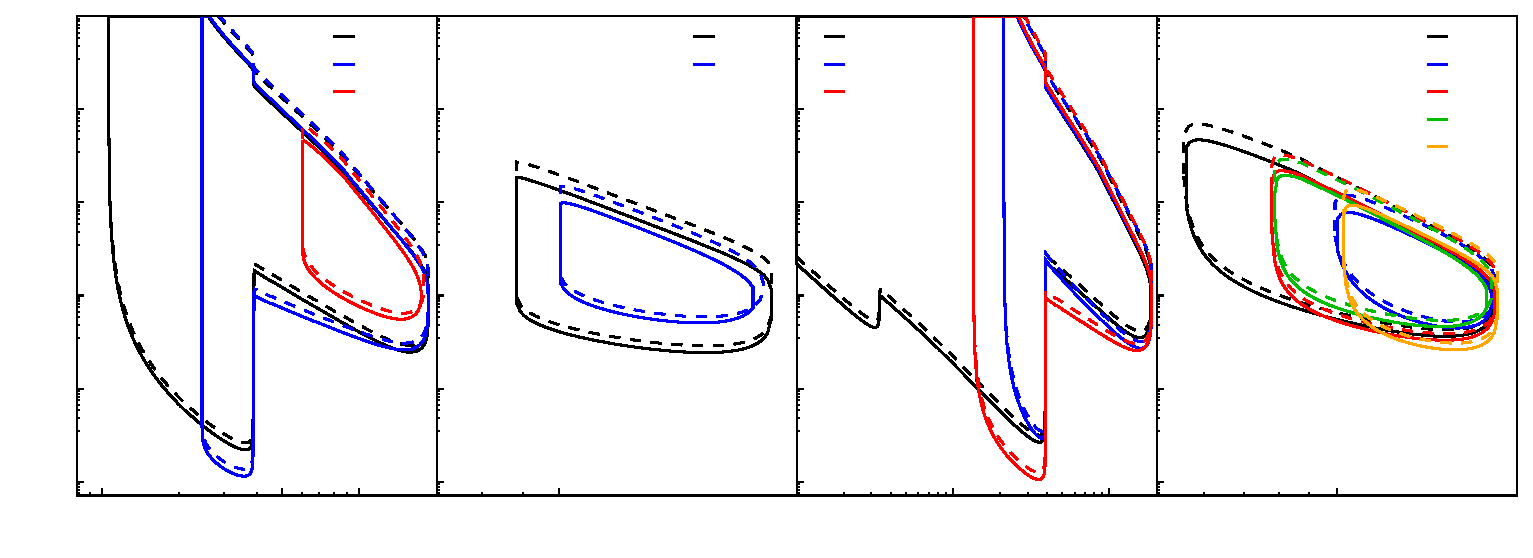
\includegraphics{pics/sensmulti_MT2_real}}%
    \gplfronttext
  \end{picture}%
\endgroup
}}
	\vspace{0.05em}

	%{\resizebox{\linewidth}{!}{\input{pics/sens_TE.tex}}}
	{\resizebox{\linewidth}{!}{% GNUPLOT: LaTeX picture with Postscript
\begingroup
  \makeatletter
  \providecommand\color[2][]{%
    \GenericError{(gnuplot) \space\space\space\@spaces}{%
      Package color not loaded in conjunction with
      terminal option `colourtext'%
    }{See the gnuplot documentation for explanation.%
    }{Either use 'blacktext' in gnuplot or load the package
      color.sty in LaTeX.}%
    \renewcommand\color[2][]{}%
  }%
  \providecommand\includegraphics[2][]{%
    \GenericError{(gnuplot) \space\space\space\@spaces}{%
      Package graphicx or graphics not loaded%
    }{See the gnuplot documentation for explanation.%
    }{The gnuplot epslatex terminal needs graphicx.sty or graphics.sty.}%
    \renewcommand\includegraphics[2][]{}%
  }%
  \providecommand\rotatebox[2]{#2}%
  \@ifundefined{ifGPcolor}{%
    \newif\ifGPcolor
    \GPcolortrue
  }{}%
  \@ifundefined{ifGPblacktext}{%
    \newif\ifGPblacktext
    \GPblacktexttrue
  }{}%
  % define a \g@addto@macro without @ in the name:
  \let\gplgaddtomacro\g@addto@macro
  % define empty templates for all commands taking text:
  \gdef\gplbacktext{}%
  \gdef\gplfronttext{}%
  \makeatother
  \ifGPblacktext
    % no textcolor at all
    \def\colorrgb#1{}%
    \def\colorgray#1{}%
  \else
    % gray or color?
    \ifGPcolor
      \def\colorrgb#1{\color[rgb]{#1}}%
      \def\colorgray#1{\color[gray]{#1}}%
      \expandafter\def\csname LTw\endcsname{\color{white}}%
      \expandafter\def\csname LTb\endcsname{\color{black}}%
      \expandafter\def\csname LTa\endcsname{\color{black}}%
      \expandafter\def\csname LT0\endcsname{\color[rgb]{1,0,0}}%
      \expandafter\def\csname LT1\endcsname{\color[rgb]{0,1,0}}%
      \expandafter\def\csname LT2\endcsname{\color[rgb]{0,0,1}}%
      \expandafter\def\csname LT3\endcsname{\color[rgb]{1,0,1}}%
      \expandafter\def\csname LT4\endcsname{\color[rgb]{0,1,1}}%
      \expandafter\def\csname LT5\endcsname{\color[rgb]{1,1,0}}%
      \expandafter\def\csname LT6\endcsname{\color[rgb]{0,0,0}}%
      \expandafter\def\csname LT7\endcsname{\color[rgb]{1,0.3,0}}%
      \expandafter\def\csname LT8\endcsname{\color[rgb]{0.5,0.5,0.5}}%
    \else
      % gray
      \def\colorrgb#1{\color{black}}%
      \def\colorgray#1{\color[gray]{#1}}%
      \expandafter\def\csname LTw\endcsname{\color{white}}%
      \expandafter\def\csname LTb\endcsname{\color{black}}%
      \expandafter\def\csname LTa\endcsname{\color{black}}%
      \expandafter\def\csname LT0\endcsname{\color{black}}%
      \expandafter\def\csname LT1\endcsname{\color{black}}%
      \expandafter\def\csname LT2\endcsname{\color{black}}%
      \expandafter\def\csname LT3\endcsname{\color{black}}%
      \expandafter\def\csname LT4\endcsname{\color{black}}%
      \expandafter\def\csname LT5\endcsname{\color{black}}%
      \expandafter\def\csname LT6\endcsname{\color{black}}%
      \expandafter\def\csname LT7\endcsname{\color{black}}%
      \expandafter\def\csname LT8\endcsname{\color{black}}%
    \fi
  \fi
    \setlength{\unitlength}{0.0500bp}%
    \ifx\gptboxheight\undefined%
      \newlength{\gptboxheight}%
      \newlength{\gptboxwidth}%
      \newsavebox{\gptboxtext}%
    \fi%
    \setlength{\fboxrule}{0.5pt}%
    \setlength{\fboxsep}{1pt}%
\begin{picture}(14400.00,5040.00)%
    \gplgaddtomacro\gplbacktext{%
      \csname LTb\endcsname%%
      \put(444,574){\makebox(0,0)[r]{\strut{}\np{e-10}}}%
      \put(444,1467){\makebox(0,0)[r]{\strut{}\np{e-8}}}%
      \put(444,2360){\makebox(0,0)[r]{\strut{}\np{e-6}}}%
      \put(444,3253){\makebox(0,0)[r]{\strut{}\np{e-4}}}%
      \put(444,4146){\makebox(0,0)[r]{\strut{}\np{e-2}}}%
      \put(444,5039){\makebox(0,0)[r]{\strut{}\np{e0}}}%
      \put(2543,220){\makebox(0,0){\strut{}$0.5$}}%
      \put(816,220){\makebox(0,0){\strut{}$0.1$}}%
      \put(3287,220){\makebox(0,0){\strut{}$1$}}%
    }%
    \gplgaddtomacro\gplfronttext{%
      \csname LTb\endcsname%%
      \put(-436,2739){\rotatebox{-270}{\makebox(0,0){\strut{}$|U_{e N} U_{\tau N}|^2$}}}%
      \put(2303,-110){\makebox(0,0){\strut{}Mass (GeV)}}%
      \csname LTb\endcsname%%
      \put(3371,4844){\makebox(0,0)[l]{\strut{}$\nu e\mu$}}%
      \csname LTb\endcsname%%
      \put(3371,4580){\makebox(0,0)[l]{\strut{}$e\pi$}}%
      \csname LTb\endcsname%%
      \put(3371,4316){\makebox(0,0)[l]{\strut{}$e K$}}%
    }%
    \gplgaddtomacro\gplbacktext{%
      \csname LTb\endcsname%%
      \put(3900,574){\makebox(0,0)[r]{\strut{}}}%
      \put(3900,1467){\makebox(0,0)[r]{\strut{}}}%
      \put(3900,2360){\makebox(0,0)[r]{\strut{}}}%
      \put(3900,3253){\makebox(0,0)[r]{\strut{}}}%
      \put(3900,4146){\makebox(0,0)[r]{\strut{}}}%
      \put(3900,5039){\makebox(0,0)[r]{\strut{}}}%
      \put(5206,220){\makebox(0,0){\strut{}$1$}}%
    }%
    \gplgaddtomacro\gplfronttext{%
      \csname LTb\endcsname%%
      \put(5759,-110){\makebox(0,0){\strut{}Mass (GeV)}}%
      \csname LTb\endcsname%%
      \put(6827,4844){\makebox(0,0)[l]{\strut{}$e\rho$}}%
      \csname LTb\endcsname%%
      \put(6827,4580){\makebox(0,0)[l]{\strut{}$e K^*$}}%
    }%
    \gplgaddtomacro\gplbacktext{%
      \csname LTb\endcsname%%
      \put(7355,574){\makebox(0,0)[r]{\strut{}}}%
      \put(7355,1467){\makebox(0,0)[r]{\strut{}}}%
      \put(7355,2360){\makebox(0,0)[r]{\strut{}}}%
      \put(7355,3253){\makebox(0,0)[r]{\strut{}}}%
      \put(7355,4146){\makebox(0,0)[r]{\strut{}}}%
      \put(7355,5039){\makebox(0,0)[r]{\strut{}}}%
      \put(7487,220){\makebox(0,0){\strut{}$0.01$}}%
      \put(8989,220){\makebox(0,0){\strut{}$0.1$}}%
      \put(10491,220){\makebox(0,0){\strut{}$1$}}%
    }%
    \gplgaddtomacro\gplfronttext{%
      \csname LTb\endcsname%%
      \put(9215,-110){\makebox(0,0){\strut{}Mass (GeV)}}%
      \csname LTb\endcsname%%
      \put(8078,4844){\makebox(0,0)[l]{\strut{}$\nu e e$}}%
      \csname LTb\endcsname%%
      \put(8078,4580){\makebox(0,0)[l]{\strut{}$\nu\mu\mu$}}%
      \csname LTb\endcsname%%
      \put(8078,4316){\makebox(0,0)[l]{\strut{}$\nu\pi^0$}}%
    }%
    \gplgaddtomacro\gplbacktext{%
      \csname LTb\endcsname%%
      \put(10812,574){\makebox(0,0)[r]{\strut{}}}%
      \put(10812,1467){\makebox(0,0)[r]{\strut{}}}%
      \put(10812,2360){\makebox(0,0)[r]{\strut{}}}%
      \put(10812,3253){\makebox(0,0)[r]{\strut{}}}%
      \put(10812,4146){\makebox(0,0)[r]{\strut{}}}%
      \put(10812,5039){\makebox(0,0)[r]{\strut{}}}%
      \put(14399,220){\makebox(0,0){\strut{}$2$}}%
      \put(12672,220){\makebox(0,0){\strut{}$1$}}%
    }%
    \gplgaddtomacro\gplfronttext{%
      \csname LTb\endcsname%%
      \put(12671,-110){\makebox(0,0){\strut{}Mass (GeV)}}%
      \csname LTb\endcsname%%
      \put(13871,4844){\makebox(0,0)[l]{\strut{}$\nu\eta$}}%
      \csname LTb\endcsname%%
      \put(13871,4580){\makebox(0,0)[l]{\strut{}$\nu\eta'$}}%
      \csname LTb\endcsname%%
      \put(13871,4316){\makebox(0,0)[l]{\strut{}$\nu\rho^0$}}%
      \csname LTb\endcsname%%
      \put(13871,4052){\makebox(0,0)[l]{\strut{}$\nu\omega$}}%
      \csname LTb\endcsname%%
      \put(13871,3788){\makebox(0,0)[l]{\strut{}$\nu\phi$}}%
    }%
    \gplbacktext
    \put(0,0){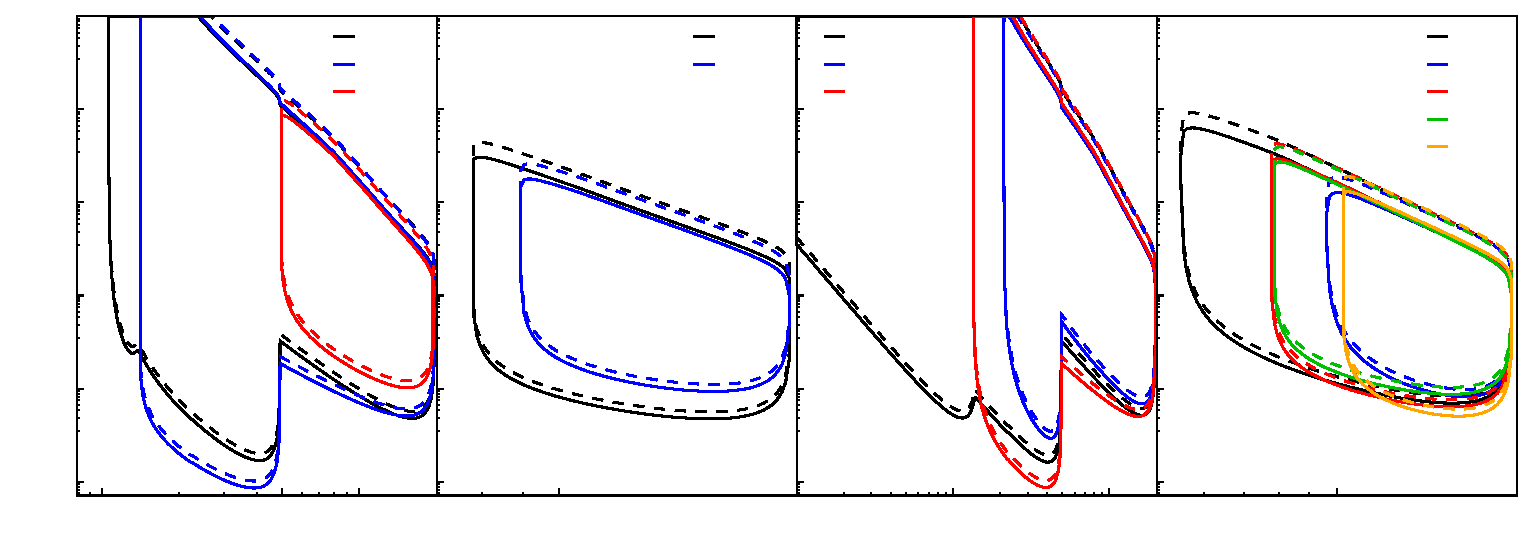
\includegraphics{pics/sensmulti_TE2_real}}%
    \gplfronttext
  \end{picture}%
\endgroup
}}
	\caption[Sensitivity regions to individual channels for two dominant mixings]%
		{The 90\,\% C.L. sensitivity regions to individual channels for two dominant mixings %
		$|U_{e N}^* U_{\mu N}|$ (top), $|U_{\mu N}^* U_{\tau N}|$ (middle), and $|U_{e N}^* U_{\tau N}|$ (bottom) are presented.
		All the modes considered in this work are shown here, but no background analysis is reported.
		As before, the solid lines correspond to the analysis with Majorana neutrinos, the dashed lines with Dirac neutrino.}
	\label{fig:senseMix}
\end{figure}

The bounds in a scenario in which two mixing elements are comparable and dominant over the third one are presented in this section.
This case complements the previous analysis in \refsec{sec:dominant} as, by searching for HNL decays, %
the experiment can constrain certain combinations of the mixing elements.
This can happen when the neutrino is produced via one mixing and decays via another one, %
or when both mixing elements play a role in production and decay.
For instance, the decay $K^+ \to \mu^+ N$ yields heavy neutrinos with a flux proportional to %
$|U_{\mu N}|^2$, but they can afterwards decay into the channel $\nu e^+ e^-$ also via the electronic or the tau mixing.
It is important to highlight that in the case in which one mixing is responsible %
for the production and a different mixing for the decay %
then number of events is proportional to the product of the mixings %
$|U_{\alpha N}||U_{\beta N}|$ if the studied channel is CC--mediated.
However, if the decay channel is also sensitive to a NC exchange, the number of events is instead proportional to %
$|U_{\alpha N}|\sqrt{|U_{\alpha N}|^2 + |U_{\beta N}|^2}$.
In the remainder of this section, the combination of two mixings will be denoted by $|U_{\alpha N}^* U_{\beta N}|$ %
for comparing bounds and sensitivity plots.

%However, if two mixings are non-zero, nothing prevents the production and the decay to be mediated by both of them. 
The combinations of mixing terms is relevant to charged Lepton Flavour Violating (cLFV) %
decays or flavour changing neutral current processes %
which can be enhanced in presence of nearly-sterile neutrinos.
For example, the well-known decay $\mu^+ \to e^+ \gamma$ has a branching ratio which is sensitive to extra neutrino states.
This reads
\begin{equation}
	\label{eq:meg}
	\text{Br}(\mu^+ \to e^+ \gamma) = \frac{3 \alpha}{32 \pi} \abs{\sum_i \hat{U}_{\mu i}^*\, \hat{U}_{e i}\,G\qty(\frac{m_i^2}{M_W^2})} \ ,
\end{equation}
where $G(x)$ is the loop function of the process~\cite{Ilakovac:1994kj}.
The current upper limit is set by the MEG experiment to be %
$\text{Br}(\mu^+ \to e^+\gamma) < \np{4.2e-13}$~\cite{TheMEG:2016wtm}.
Despite being one of the best constrained cLFV process, the bounds on $|U_{e N}^* U_{\mu N}|$ are not as good as the ones imposed %
by other processes, like $\mu \to e e e$ or $\mu - e$ conversion on nuclei~\cite{Alonso:2012ji}.
For instance, the constraint from conversion on Au is $|U_{e N}^* U_{\mu N}| < \np{1.6e-5}$ %
for HNL masses larger than 0.1\,GeV~\cite{Deshpande:2011uv}.
The branching ratio of other cLFV channels, like $\tau^\pm \to e^\pm \gamma$ or $\tau^\pm \to \mu^\pm \gamma$ %
cannot be as simply determined and so the bounds achieved on the combination of heavy neutrino mixings are expected %
to be less stringent~\cite{Buras:2010cp, Abada:2016vzu}.
Stronger bounds come from the study of three-body decays of charm and bottom mesons to charged leptons with different flavour %
and tau decays to pseudoscalar mesons and a charged lepton: from the search for %
the decay $K \to e \mu \pi$ the bound $|U_{e N}^* U_{\mu N}| < \np{e-9}$ is reached for masses %
$0.15\,\text{GeV}\lesssim m_N \lesssim 0.50\,\text{GeV}$;
the decays $\tau \to e \pi \pi$ and $\tau \to \mu \pi\pi$ set the limits %
$|U_{e N}^* U_{\tau N}|, |U_{\mu N}^* U_{\tau N}| < \np{5e-6}$ for the respective mass ranges %
$0.14\,\text{GeV}\lesssim m_N \lesssim 1.7\,\text{GeV}$ and %
$0.24\,\text{GeV}\lesssim m_N \lesssim 1.7\,\text{GeV}$~\cite{Helo:2010cw}.



Instead of dealing with a three-dimensional parameter scan of the neutrino mass and two mixing angles, %
the study is simplified by assigning the same value to the two mixing parameters under consideration, %
for which the number of HNL decays is maximal.
The number of events is then reported as a function of the neutrino mass and the combination $|U_{\alpha N}^* U_{\beta N}|$.
The results for all channels considered in this work are shown in~\reffig{fig:senseMix}.
The best constraints come again from two-body semileptonic decays for all mixing combinations, %
the lowest upper limits being $|U_{e N}^* U_{\mu N}| < \np{6e-11}$ at $m_N \simeq 0.36$\,GeV, %
$|U_{\mu N}^* U_{\tau N}| < \np{1.3e-10}$ at $m_N \simeq 0.35$\,GeV, %
and $|U_{\tau N}^* U_{e N}| < \np{7e-11}$ at $m_N \simeq 0.39$\,GeV.
Amongst the three-body leptonic decay channels, $N\to\nu e e$ has the best sensitivity for masses $m_N < m_{K^0}$, %
but the mode $N\to \nu e^\mp \mu^\pm$ can be actually more constraining at higher masses.
Regarding the channels available only above the kaon mass threshold, decays to pseudoscalar mesons are the most sensitive %
between CC processes, whereas the decay $N \to \nu \phi$ gives the best constraint of the NC--mediated channels.

\section{Mass model constraints from DUNE ND}
\label{sec:combined}

%Finally, we make a comparison of this analysis with previous and recent results of beam dump experiment.
%and explain the how the experiment %
%can explore the parameter spaces of different neutrino mass models in the next section, \ref{sec:combined}.

From the results presented in the previous section, the DUNE ND will be sensitive to very low couplings %
for experimentally accessible mass values.
These points of the parameter space correspond to regions viable in some realisations of low scale neutrino mass models.
In view of the discussion regarding seesaw models in \refsec{sec:model}, %
a random scan of mass matrices is performed to define such regions of the parameter space.
Three minimal ISS scenarios are chosen requiring they predict a HNL with a mass accessible %
by the experiment and that satisfy the experimental evidence of neutrino oscillation~\cite{Abada:2014vea}.
Following the notation introduce in \refcha{cha:mass_models}, in the first two cases %
the heavy neutrino under study belongs to the lightest pseudo-Dirac pair of an ISS\,(2,2) and an ISS\,(2,3) realisation; %
the third scenario is an ISS\,(2,3) case in which the fourth massless state becomes %
a Majorana neutrino in the \mbox{MeV--GeV} region thanks to a high LNV parameter.
The details of this analysis are reported in this section, together with the overall sensitivities of DUNE ND to %
heavy neutrino discovery and low scale mass models. 
A~comparison with future experiments is also included.

\subsection{Mass model scan}

%The DUNE experiment will be very sensitive to regions of the parameter space of interest with respect to low scale seesaw models.
Neutrino mass matrices with the same structure of \refeq{eq:iss_matrix_lnv} are randomly generated and numerically diagonalised.
The number of physical parameters of a ISS\,$(a,b)$ mass matrix is found to be $n_p = 7a + b +2\, a\,b$~\cite{Abada:2014vea}. %
A basis in which $m_D$ has complex entries but three of which are real %
and $M_R$ is diagonal and real can be chosen without loss of generality.
If the matrix entries respect the hierarchy \mbox{$\mu \ll m_D \ll M_R$}, the mass spectrum in %
the LNC limit is principally given by the diagonal values of $M_R$.
The matrix is then perturbed to achieve the three minimal ISS scenarios introduced above; %
the randomly generated mass matrix $\mathcal{M}$ %
is diagonalised using the Jacobi Singular Value Decomposition (SVD) as implemented in the Eigen library~\cite{eigenweb}.
The Takagi decomposition, %
\begin{equation}
	\hat{U}^T \mathcal{M}\, \hat{U} = \text{diag}(m_1, m_2, m_3, ...)\ ,
\end{equation}
is retrieved starting from the SVD decomposition $\mathcal{M} = V \Sigma U^\dagger$, %
from which the singular values $\Sigma$ are the non-negative square roots of the eigenvalues of $\mathcal{M}^\dagger \mathcal{M}$ %
and the unitary matrix is $\hat{U} = U \rho^\dagger$, where $\rho = (U^T V)^\frac{1}{2}$ is a unitary phase matrix.

Only matrices satisfying the current constraints on heavy neutral fermions are taken in account.
The first requirement is that the eigenvalues must give the correct mass squared splittings %
compatible within 3$\sigma$ with the measured values~\cite{Esteban:2018azc}.
The condition of matching also the measured mixing angles is relaxed because %
the entries of the PMNS matrix are the result of the random structure of $m_D$ and $\mu$.
Constraints on the unitarity of the mixing matrix are applied instead.
The deviation from unitarity are quantified by the following Hermitian matrix:
\begin{equation}
	\varepsilon_{\alpha \beta} \equiv |\delta_{\alpha \beta} - (\mathcal{U}\,\mathcal{U}^\dagger)_{\alpha \beta}| = %
	\abs{\sum_{i=4}^n \hat{U}_{\alpha i} \hat{U}_{\beta i}^*}\ .
\end{equation}
The non-unitarity of the PMNS matrix has been assessed in various experiments, and the constraints depend upon the mass scale of averaged out neutrinos.
For neutrino masses below the GeV scale, but heavy enough to decouple from flavour oscillations, %
non-unitarity effects are tested in neutrino oscillation experiment as an overall normalisation.
If the neutrino mass is above the GeV scale, electroweak precision experiments provide strong constraints on non-unitarity.
The limits are summarised below (from~\refref{Antusch:2008tz, Fernandez-Martinez:2016lgt, Blennow:2016jkn})
\begin{align}
	&\varepsilon_{\alpha \beta} <
	\begin{pmatrix}
		\np{2.4e-2}	& \np{1.3e-2}	& \np{3.5e-2}	\\
		\cdot		& \np{2.2e-2}	& \np{6.0e-3}	\\
		\cdot		& \cdot		& \np{1.0e-1}
	\end{pmatrix}\quad 
	\text{if 10\,eV} \lesssim m_N \lesssim \text{1\,GeV}\ ,\\
	&\varepsilon_{\alpha \beta} <
	\begin{pmatrix}
		\np{1.3e-3}	& \np{1.2e-5}	& \np{1.4e-3}	\\
		\cdot		& \np{2.2e-4}	& \np{6.0e-4}	\\
		\cdot		& \cdot		& \np{2.8e-3}
	\end{pmatrix}\quad
	\text{if}\ m_N \gtrsim \text{1\,GeV}\ .
\end{align}

The $\mu$ entries of the ISS matrices naturally lead to lepton flavour and lepton number violating processes.
The most studied LFV process is the decay rate of \mbox{$\mu^+ \to e^+\gamma$}, the branching ratio of which is given in \refeq{eq:meg}.
The current upper limit on the branching ratio is \np{4.2e-13}, but a future upgrade of the experiment %
foresees to reach a limit lower than \np{5e-14}.

Heavy neutrinos in a ISS model also contribute to the neutrinoless double beta decay.
The effective neutrino mass $m_{\beta\beta}$ receives further corrections with respect %
to the standard expression as
\begin{equation}
	m_{\beta\beta} \simeq \abs{\sum_i \hat{U}_{e i}^2 \frac{p^2\,m_i}{p^2 - m_i^2}}
\end{equation}
where $p^2 \simeq -\np{0.015}$\,GeV\tapi{2} is the typical virtual momentum of the exchanged neutrino.
The~contribution from masses above the 0.1\,GeV scale drops as $\flatfrac{1}{m^2_i}$ while it is constant for masses below~\cite{Blennow:2010th}.
It is interesting to note that the contributions given by pseudo-Dirac pairs are subject to partial cancellation, regulated by the LNV parameters.
In the LNC limit, the cancellation is maximum and the paired states do not take part in the $0\nu\beta\beta$ process.
The latest result from the KamLAND-Zen experiment is interpreted as~\mbox{$m_{\beta\beta} < 61$\,meV}~\cite{KamLAND-Zen:2016pfg}.
%The latest result from the GERDA experiment~\cite{Agostini:2017iyd} is interpreted as $m_{\beta\beta} < 150$\,meV.

For the first two ISS scenarios the allowed ranges span in the space %
\mbox{$m_D \sim 10^{[3,6]}$\,eV}, \mbox{$M_R \sim 10^{[6,15]}$\,eV}, $\mu \sim 10^{[-4,1]}$\,eV.
Each matrix generated is verified to respect the \emph{naturalness condition} in the 't Hooft sense~\cite{tHooft:1980xss} %
and that the mass spectrum presents a mass state accessible by the DUNE experiment.
For the third ISS case, large entries of the submatrix $\mu$ are necessary to give the Majorana state a mass that %
can be probed by the experiment.
The ranges of \mbox{$m_D \sim 10^{[3,10]}$\,eV}, $M_R \sim 10^{[7,15]}$\,eV, $\mu \sim 10^{[4,9]}$\,eV to respect %
the constraints.
The hierarchy and naturalness conditions are relaxed in this case.
%It is found that the block $\mu_R$ does not influence the final mass spectrum; %
%it usually gives contribution to the light neutrino masses at the loop level, in a region below the GeV scale that has been already excluded by experiments.
%The neutrino masses and the mixing elements are extracted from the mass matrices that survive all the experimental constraints.
The resulting points in the space $(m_N, |U_{\alpha N}|^2)$ are clustered together and the regions defined are overlaid in \reffig{fig:sensAll}.
Any combination of mass and mixing element inside these areas can be justified by a valid neutrino mass matrix %
which can explain the light neutrino masses and survive the experimental constraints.
The pseudo-Dirac pairs from the ISS\,(2,2) and ISS\,(2,3) scenarios give very similar regions, %
but Majorana states from the ISS\,(2,3) realisation can only be generated with very small couplings.
A type I seesaw band, corresponding to light neutrino mass between 20~meV and 200~meV, %
is highlighted in the figure for comparison.




\subsection{Overall sensitivity}

The overall sensitivity of DUNE ND to the discovery of HNL is defined here as the combination of the sensitivities %
to some selected channels and presented in \reffig{fig:sensAll}.
These channels are $N \to \nu e^+ e^-$, $\nu e^\pm \mu^\mp$, $\nu \mu^+\mu^-$, $\nu\pi^0$, $e^\mp\pi^\pm$, and $\mu^\mp\pi^\pm$, %
and are preferred because of their good discovery prospect, for which a background study has also been carried out.
They all give strong sensitivities, especially for masses below 0.5\,GeV, as shown in \refsec{sec:results}.
Their reach is due to high branching ratios and the HNL flux being more intense at such masses.
Also, the final state particles are all well-studied particles, most of which leave tracks in the detector %
that are easy to reconstruct, therefore allowing the background to be controlled with sufficient precision.
The neutrino spectrum component coming from the $D_s$ meson allows for a weaker sensitivity %
to masses above the neutral kaon mass.
The sensitivity study is conducted for the two scenarios in which either a Majorana or a Dirac neutrino is the decaying particle.


\begin{figure}
	\centering
	\noindent\makebox[\textwidth][c]{%
		\begin{minipage}{1.0\linewidth}
			%\hspace{-1.0em}
			{\resizebox{0.5\linewidth}{!}{% GNUPLOT: LaTeX picture with Postscript
\begingroup
  \makeatletter
  \providecommand\color[2][]{%
    \GenericError{(gnuplot) \space\space\space\@spaces}{%
      Package color not loaded in conjunction with
      terminal option `colourtext'%
    }{See the gnuplot documentation for explanation.%
    }{Either use 'blacktext' in gnuplot or load the package
      color.sty in LaTeX.}%
    \renewcommand\color[2][]{}%
  }%
  \providecommand\includegraphics[2][]{%
    \GenericError{(gnuplot) \space\space\space\@spaces}{%
      Package graphicx or graphics not loaded%
    }{See the gnuplot documentation for explanation.%
    }{The gnuplot epslatex terminal needs graphicx.sty or graphics.sty.}%
    \renewcommand\includegraphics[2][]{}%
  }%
  \providecommand\rotatebox[2]{#2}%
  \@ifundefined{ifGPcolor}{%
    \newif\ifGPcolor
    \GPcolortrue
  }{}%
  \@ifundefined{ifGPblacktext}{%
    \newif\ifGPblacktext
    \GPblacktexttrue
  }{}%
  % define a \g@addto@macro without @ in the name:
  \let\gplgaddtomacro\g@addto@macro
  % define empty templates for all commands taking text:
  \gdef\gplbacktext{}%
  \gdef\gplfronttext{}%
  \makeatother
  \ifGPblacktext
    % no textcolor at all
    \def\colorrgb#1{}%
    \def\colorgray#1{}%
  \else
    % gray or color?
    \ifGPcolor
      \def\colorrgb#1{\color[rgb]{#1}}%
      \def\colorgray#1{\color[gray]{#1}}%
      \expandafter\def\csname LTw\endcsname{\color{white}}%
      \expandafter\def\csname LTb\endcsname{\color{black}}%
      \expandafter\def\csname LTa\endcsname{\color{black}}%
      \expandafter\def\csname LT0\endcsname{\color[rgb]{1,0,0}}%
      \expandafter\def\csname LT1\endcsname{\color[rgb]{0,1,0}}%
      \expandafter\def\csname LT2\endcsname{\color[rgb]{0,0,1}}%
      \expandafter\def\csname LT3\endcsname{\color[rgb]{1,0,1}}%
      \expandafter\def\csname LT4\endcsname{\color[rgb]{0,1,1}}%
      \expandafter\def\csname LT5\endcsname{\color[rgb]{1,1,0}}%
      \expandafter\def\csname LT6\endcsname{\color[rgb]{0,0,0}}%
      \expandafter\def\csname LT7\endcsname{\color[rgb]{1,0.3,0}}%
      \expandafter\def\csname LT8\endcsname{\color[rgb]{0.5,0.5,0.5}}%
    \else
      % gray
      \def\colorrgb#1{\color{black}}%
      \def\colorgray#1{\color[gray]{#1}}%
      \expandafter\def\csname LTw\endcsname{\color{white}}%
      \expandafter\def\csname LTb\endcsname{\color{black}}%
      \expandafter\def\csname LTa\endcsname{\color{black}}%
      \expandafter\def\csname LT0\endcsname{\color{black}}%
      \expandafter\def\csname LT1\endcsname{\color{black}}%
      \expandafter\def\csname LT2\endcsname{\color{black}}%
      \expandafter\def\csname LT3\endcsname{\color{black}}%
      \expandafter\def\csname LT4\endcsname{\color{black}}%
      \expandafter\def\csname LT5\endcsname{\color{black}}%
      \expandafter\def\csname LT6\endcsname{\color{black}}%
      \expandafter\def\csname LT7\endcsname{\color{black}}%
      \expandafter\def\csname LT8\endcsname{\color{black}}%
    \fi
  \fi
    \setlength{\unitlength}{0.0500bp}%
    \ifx\gptboxheight\undefined%
      \newlength{\gptboxheight}%
      \newlength{\gptboxwidth}%
      \newsavebox{\gptboxtext}%
    \fi%
    \setlength{\fboxrule}{0.5pt}%
    \setlength{\fboxsep}{1pt}%
\begin{picture}(7200.00,5040.00)%
    \gplgaddtomacro\gplbacktext{%
      \csname LTb\endcsname%%
      \put(849,1039){\makebox(0,0)[r]{\strut{}$10^{-10}$}}%
      \csname LTb\endcsname%%
      \put(849,1928){\makebox(0,0)[r]{\strut{}$10^{-8}$}}%
      \csname LTb\endcsname%%
      \put(849,2817){\makebox(0,0)[r]{\strut{}$10^{-6}$}}%
      \csname LTb\endcsname%%
      \put(849,3706){\makebox(0,0)[r]{\strut{}$10^{-4}$}}%
      \csname LTb\endcsname%%
      \put(849,4595){\makebox(0,0)[r]{\strut{}$10^{-2}$}}%
      \csname LTb\endcsname%%
      \put(2844,409){\makebox(0,0){\strut{}0.05}}%
      \csname LTb\endcsname%%
      \put(5552,409){\makebox(0,0){\strut{}0.5}}%
      \csname LTb\endcsname%%
      \put(7183,409){\makebox(0,0){\strut{}2}}%
      \csname LTb\endcsname%%
      \put(951,409){\makebox(0,0){\strut{}0.01}}%
      \csname LTb\endcsname%%
      \put(3659,409){\makebox(0,0){\strut{}0.1}}%
      \csname LTb\endcsname%%
      \put(6368,409){\makebox(0,0){\strut{}1}}%
    }%
    \gplgaddtomacro\gplfronttext{%
      \csname LTb\endcsname%%
      \put(153,2817){\rotatebox{-270}{\makebox(0,0){\strut{}$|U_{e N}|^2$}}}%
      \csname LTb\endcsname%%
      \put(4067,130){\makebox(0,0){\strut{}Mass $m_N$ (GeV)}}%
      \csname LTb\endcsname%%
      \put(4151,3713){\makebox(0,0)[l]{\strut{}FASER}}%
      \csname LTb\endcsname%%
      \put(4151,3917){\makebox(0,0)[l]{\strut{}MATHUSLA}}%
      \csname LTb\endcsname%%
      \put(4151,4121){\makebox(0,0)[l]{\strut{}NA62}}%
      \csname LTb\endcsname%%
      \put(4151,4325){\makebox(0,0)[l]{\strut{}SHiP}}%
      \csname LTb\endcsname%%
      \put(4151,4529){\makebox(0,0)[l]{\strut{}SBND}}%
      \csname LTb\endcsname%%
      \put(4151,4733){\makebox(0,0)[l]{\strut{}DUNE}}%
      \csname LTb\endcsname%%
      \put(4151,4937){\makebox(0,0)[l]{\strut{} }}%
      \csname LTb\endcsname%%
      \put(849,1039){\makebox(0,0)[r]{\strut{}$10^{-10}$}}%
      \csname LTb\endcsname%%
      \put(849,1928){\makebox(0,0)[r]{\strut{}$10^{-8}$}}%
      \csname LTb\endcsname%%
      \put(849,2817){\makebox(0,0)[r]{\strut{}$10^{-6}$}}%
      \csname LTb\endcsname%%
      \put(849,3706){\makebox(0,0)[r]{\strut{}$10^{-4}$}}%
      \csname LTb\endcsname%%
      \put(849,4595){\makebox(0,0)[r]{\strut{}$10^{-2}$}}%
      \csname LTb\endcsname%%
      \put(2844,409){\makebox(0,0){\strut{}0.05}}%
      \csname LTb\endcsname%%
      \put(5552,409){\makebox(0,0){\strut{}0.5}}%
      \csname LTb\endcsname%%
      \put(7183,409){\makebox(0,0){\strut{}2}}%
      \csname LTb\endcsname%%
      \put(951,409){\makebox(0,0){\strut{}0.01}}%
      \csname LTb\endcsname%%
      \put(3659,409){\makebox(0,0){\strut{}0.1}}%
      \csname LTb\endcsname%%
      \put(6368,409){\makebox(0,0){\strut{}1}}%
      \csname LTb\endcsname%%
      \put(2844,4284){\makebox(0,0){\strut{}\textbf{Excluded}}}%
      \csname LTb\endcsname%%
      \put(1766,996){\makebox(0,0){\strut{}\textbf{Weyl state}}}%
      \csname LTb\endcsname%%
      \put(1766,2373){\makebox(0,0){\strut{}\textbf{\shortstack{Pseudo-Dirac\\pair}}}}%
      \csname LTb\endcsname%%
      \put(2844,1484){\rotatebox{-5}{\makebox(0,0){\strut{}\textbf{Type I}}}}%
    }%
    \gplbacktext
    \put(0,0){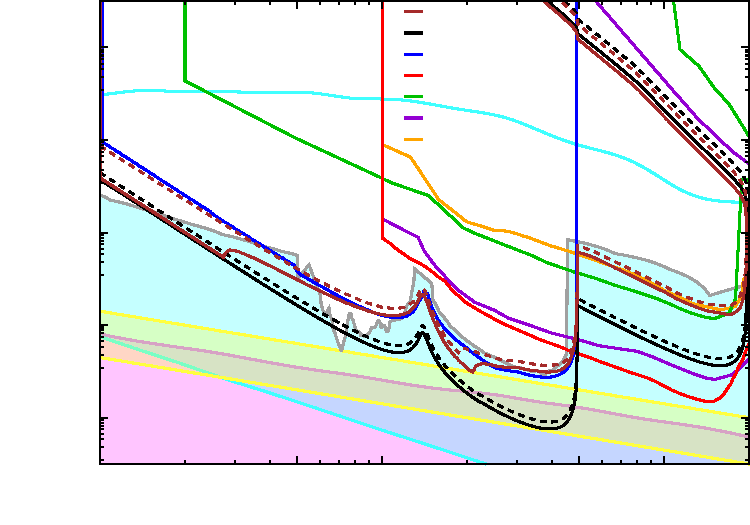
\includegraphics{pics/DUNE_HNL_E_real}}%
    \gplfronttext
  \end{picture}%
\endgroup
}}
			%\hspace{-0.5em}
			{\resizebox{0.5\linewidth}{!}{% GNUPLOT: LaTeX picture with Postscript
\begingroup
  \makeatletter
  \providecommand\color[2][]{%
    \GenericError{(gnuplot) \space\space\space\@spaces}{%
      Package color not loaded in conjunction with
      terminal option `colourtext'%
    }{See the gnuplot documentation for explanation.%
    }{Either use 'blacktext' in gnuplot or load the package
      color.sty in LaTeX.}%
    \renewcommand\color[2][]{}%
  }%
  \providecommand\includegraphics[2][]{%
    \GenericError{(gnuplot) \space\space\space\@spaces}{%
      Package graphicx or graphics not loaded%
    }{See the gnuplot documentation for explanation.%
    }{The gnuplot epslatex terminal needs graphicx.sty or graphics.sty.}%
    \renewcommand\includegraphics[2][]{}%
  }%
  \providecommand\rotatebox[2]{#2}%
  \@ifundefined{ifGPcolor}{%
    \newif\ifGPcolor
    \GPcolortrue
  }{}%
  \@ifundefined{ifGPblacktext}{%
    \newif\ifGPblacktext
    \GPblacktexttrue
  }{}%
  % define a \g@addto@macro without @ in the name:
  \let\gplgaddtomacro\g@addto@macro
  % define empty templates for all commands taking text:
  \gdef\gplbacktext{}%
  \gdef\gplfronttext{}%
  \makeatother
  \ifGPblacktext
    % no textcolor at all
    \def\colorrgb#1{}%
    \def\colorgray#1{}%
  \else
    % gray or color?
    \ifGPcolor
      \def\colorrgb#1{\color[rgb]{#1}}%
      \def\colorgray#1{\color[gray]{#1}}%
      \expandafter\def\csname LTw\endcsname{\color{white}}%
      \expandafter\def\csname LTb\endcsname{\color{black}}%
      \expandafter\def\csname LTa\endcsname{\color{black}}%
      \expandafter\def\csname LT0\endcsname{\color[rgb]{1,0,0}}%
      \expandafter\def\csname LT1\endcsname{\color[rgb]{0,1,0}}%
      \expandafter\def\csname LT2\endcsname{\color[rgb]{0,0,1}}%
      \expandafter\def\csname LT3\endcsname{\color[rgb]{1,0,1}}%
      \expandafter\def\csname LT4\endcsname{\color[rgb]{0,1,1}}%
      \expandafter\def\csname LT5\endcsname{\color[rgb]{1,1,0}}%
      \expandafter\def\csname LT6\endcsname{\color[rgb]{0,0,0}}%
      \expandafter\def\csname LT7\endcsname{\color[rgb]{1,0.3,0}}%
      \expandafter\def\csname LT8\endcsname{\color[rgb]{0.5,0.5,0.5}}%
    \else
      % gray
      \def\colorrgb#1{\color{black}}%
      \def\colorgray#1{\color[gray]{#1}}%
      \expandafter\def\csname LTw\endcsname{\color{white}}%
      \expandafter\def\csname LTb\endcsname{\color{black}}%
      \expandafter\def\csname LTa\endcsname{\color{black}}%
      \expandafter\def\csname LT0\endcsname{\color{black}}%
      \expandafter\def\csname LT1\endcsname{\color{black}}%
      \expandafter\def\csname LT2\endcsname{\color{black}}%
      \expandafter\def\csname LT3\endcsname{\color{black}}%
      \expandafter\def\csname LT4\endcsname{\color{black}}%
      \expandafter\def\csname LT5\endcsname{\color{black}}%
      \expandafter\def\csname LT6\endcsname{\color{black}}%
      \expandafter\def\csname LT7\endcsname{\color{black}}%
      \expandafter\def\csname LT8\endcsname{\color{black}}%
    \fi
  \fi
    \setlength{\unitlength}{0.0500bp}%
    \ifx\gptboxheight\undefined%
      \newlength{\gptboxheight}%
      \newlength{\gptboxwidth}%
      \newsavebox{\gptboxtext}%
    \fi%
    \setlength{\fboxrule}{0.5pt}%
    \setlength{\fboxsep}{1pt}%
\begin{picture}(7200.00,5040.00)%
    \gplgaddtomacro\gplbacktext{%
      \csname LTb\endcsname%%
      \put(849,1039){\makebox(0,0)[r]{\strut{}$10^{-10}$}}%
      \csname LTb\endcsname%%
      \put(849,1928){\makebox(0,0)[r]{\strut{}$10^{-8}$}}%
      \csname LTb\endcsname%%
      \put(849,2817){\makebox(0,0)[r]{\strut{}$10^{-6}$}}%
      \csname LTb\endcsname%%
      \put(849,3706){\makebox(0,0)[r]{\strut{}$10^{-4}$}}%
      \csname LTb\endcsname%%
      \put(849,4595){\makebox(0,0)[r]{\strut{}$10^{-2}$}}%
      \csname LTb\endcsname%%
      \put(2844,409){\makebox(0,0){\strut{}0.05}}%
      \csname LTb\endcsname%%
      \put(5552,409){\makebox(0,0){\strut{}0.5}}%
      \csname LTb\endcsname%%
      \put(7183,409){\makebox(0,0){\strut{}2}}%
      \csname LTb\endcsname%%
      \put(951,409){\makebox(0,0){\strut{}0.01}}%
      \csname LTb\endcsname%%
      \put(3659,409){\makebox(0,0){\strut{}0.1}}%
      \csname LTb\endcsname%%
      \put(6368,409){\makebox(0,0){\strut{}1}}%
    }%
    \gplgaddtomacro\gplfronttext{%
      \csname LTb\endcsname%%
      \put(153,2817){\rotatebox{-270}{\makebox(0,0){\strut{}$|U_{\mu N}|^2$}}}%
      \csname LTb\endcsname%%
      \put(4067,130){\makebox(0,0){\strut{}Mass $m_N$ (GeV)}}%
      \csname LTb\endcsname%%
      \put(4348,3713){\makebox(0,0)[l]{\strut{}FASER}}%
      \csname LTb\endcsname%%
      \put(4348,3917){\makebox(0,0)[l]{\strut{}MATHUSLA}}%
      \csname LTb\endcsname%%
      \put(4348,4121){\makebox(0,0)[l]{\strut{}NA62}}%
      \csname LTb\endcsname%%
      \put(4348,4325){\makebox(0,0)[l]{\strut{}SHiP}}%
      \csname LTb\endcsname%%
      \put(4348,4529){\makebox(0,0)[l]{\strut{}SBND}}%
      \csname LTb\endcsname%%
      \put(4348,4733){\makebox(0,0)[l]{\strut{}DUNE}}%
      \csname LTb\endcsname%%
      \put(4348,4937){\makebox(0,0)[l]{\strut{} }}%
      \csname LTb\endcsname%%
      \put(849,1039){\makebox(0,0)[r]{\strut{}$10^{-10}$}}%
      \csname LTb\endcsname%%
      \put(849,1928){\makebox(0,0)[r]{\strut{}$10^{-8}$}}%
      \csname LTb\endcsname%%
      \put(849,2817){\makebox(0,0)[r]{\strut{}$10^{-6}$}}%
      \csname LTb\endcsname%%
      \put(849,3706){\makebox(0,0)[r]{\strut{}$10^{-4}$}}%
      \csname LTb\endcsname%%
      \put(849,4595){\makebox(0,0)[r]{\strut{}$10^{-2}$}}%
      \csname LTb\endcsname%%
      \put(2844,409){\makebox(0,0){\strut{}0.05}}%
      \csname LTb\endcsname%%
      \put(5552,409){\makebox(0,0){\strut{}0.5}}%
      \csname LTb\endcsname%%
      \put(7183,409){\makebox(0,0){\strut{}2}}%
      \csname LTb\endcsname%%
      \put(951,409){\makebox(0,0){\strut{}0.01}}%
      \csname LTb\endcsname%%
      \put(3659,409){\makebox(0,0){\strut{}0.1}}%
      \csname LTb\endcsname%%
      \put(6368,409){\makebox(0,0){\strut{}1}}%
      \csname LTb\endcsname%%
      \put(4737,3261){\makebox(0,0){\strut{}\textbf{Excluded}}}%
      \csname LTb\endcsname%%
      \put(1766,996){\makebox(0,0){\strut{}\textbf{Weyl state}}}%
      \csname LTb\endcsname%%
      \put(2582,2239){\makebox(0,0){\strut{}\textbf{\shortstack{Pseudo-Dirac\\pair}}}}%
      \csname LTb\endcsname%%
      \put(2844,1484){\rotatebox{-5}{\makebox(0,0){\strut{}\textbf{Type I}}}}%
    }%
    \gplbacktext
    \put(0,0){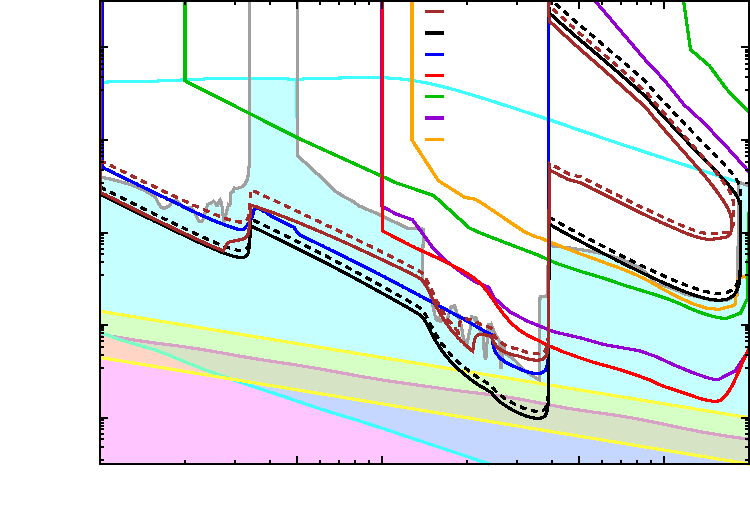
\includegraphics{pics/DUNE_HNL_M_real}}%
    \gplfronttext
  \end{picture}%
\endgroup
}}
		\end{minipage}
	}

	\vspace{0.5em}
	{\resizebox{0.5\linewidth}{!}{% GNUPLOT: LaTeX picture with Postscript
\begingroup
  \makeatletter
  \providecommand\color[2][]{%
    \GenericError{(gnuplot) \space\space\space\@spaces}{%
      Package color not loaded in conjunction with
      terminal option `colourtext'%
    }{See the gnuplot documentation for explanation.%
    }{Either use 'blacktext' in gnuplot or load the package
      color.sty in LaTeX.}%
    \renewcommand\color[2][]{}%
  }%
  \providecommand\includegraphics[2][]{%
    \GenericError{(gnuplot) \space\space\space\@spaces}{%
      Package graphicx or graphics not loaded%
    }{See the gnuplot documentation for explanation.%
    }{The gnuplot epslatex terminal needs graphicx.sty or graphics.sty.}%
    \renewcommand\includegraphics[2][]{}%
  }%
  \providecommand\rotatebox[2]{#2}%
  \@ifundefined{ifGPcolor}{%
    \newif\ifGPcolor
    \GPcolortrue
  }{}%
  \@ifundefined{ifGPblacktext}{%
    \newif\ifGPblacktext
    \GPblacktexttrue
  }{}%
  % define a \g@addto@macro without @ in the name:
  \let\gplgaddtomacro\g@addto@macro
  % define empty templates for all commands taking text:
  \gdef\gplbacktext{}%
  \gdef\gplfronttext{}%
  \makeatother
  \ifGPblacktext
    % no textcolor at all
    \def\colorrgb#1{}%
    \def\colorgray#1{}%
  \else
    % gray or color?
    \ifGPcolor
      \def\colorrgb#1{\color[rgb]{#1}}%
      \def\colorgray#1{\color[gray]{#1}}%
      \expandafter\def\csname LTw\endcsname{\color{white}}%
      \expandafter\def\csname LTb\endcsname{\color{black}}%
      \expandafter\def\csname LTa\endcsname{\color{black}}%
      \expandafter\def\csname LT0\endcsname{\color[rgb]{1,0,0}}%
      \expandafter\def\csname LT1\endcsname{\color[rgb]{0,1,0}}%
      \expandafter\def\csname LT2\endcsname{\color[rgb]{0,0,1}}%
      \expandafter\def\csname LT3\endcsname{\color[rgb]{1,0,1}}%
      \expandafter\def\csname LT4\endcsname{\color[rgb]{0,1,1}}%
      \expandafter\def\csname LT5\endcsname{\color[rgb]{1,1,0}}%
      \expandafter\def\csname LT6\endcsname{\color[rgb]{0,0,0}}%
      \expandafter\def\csname LT7\endcsname{\color[rgb]{1,0.3,0}}%
      \expandafter\def\csname LT8\endcsname{\color[rgb]{0.5,0.5,0.5}}%
    \else
      % gray
      \def\colorrgb#1{\color{black}}%
      \def\colorgray#1{\color[gray]{#1}}%
      \expandafter\def\csname LTw\endcsname{\color{white}}%
      \expandafter\def\csname LTb\endcsname{\color{black}}%
      \expandafter\def\csname LTa\endcsname{\color{black}}%
      \expandafter\def\csname LT0\endcsname{\color{black}}%
      \expandafter\def\csname LT1\endcsname{\color{black}}%
      \expandafter\def\csname LT2\endcsname{\color{black}}%
      \expandafter\def\csname LT3\endcsname{\color{black}}%
      \expandafter\def\csname LT4\endcsname{\color{black}}%
      \expandafter\def\csname LT5\endcsname{\color{black}}%
      \expandafter\def\csname LT6\endcsname{\color{black}}%
      \expandafter\def\csname LT7\endcsname{\color{black}}%
      \expandafter\def\csname LT8\endcsname{\color{black}}%
    \fi
  \fi
    \setlength{\unitlength}{0.0500bp}%
    \ifx\gptboxheight\undefined%
      \newlength{\gptboxheight}%
      \newlength{\gptboxwidth}%
      \newsavebox{\gptboxtext}%
    \fi%
    \setlength{\fboxrule}{0.5pt}%
    \setlength{\fboxsep}{1pt}%
\begin{picture}(7200.00,5040.00)%
    \gplgaddtomacro\gplbacktext{%
      \csname LTb\endcsname%%
      \put(849,595){\makebox(0,0)[r]{\strut{}$10^{-10}$}}%
      \csname LTb\endcsname%%
      \put(849,1484){\makebox(0,0)[r]{\strut{}$10^{-8}$}}%
      \csname LTb\endcsname%%
      \put(849,2373){\makebox(0,0)[r]{\strut{}$10^{-6}$}}%
      \csname LTb\endcsname%%
      \put(849,3261){\makebox(0,0)[r]{\strut{}$10^{-4}$}}%
      \csname LTb\endcsname%%
      \put(849,4150){\makebox(0,0)[r]{\strut{}$10^{-2}$}}%
      \csname LTb\endcsname%%
      \put(849,5039){\makebox(0,0)[r]{\strut{}$10^{0}$}}%
      \csname LTb\endcsname%%
      \put(2844,409){\makebox(0,0){\strut{}0.05}}%
      \csname LTb\endcsname%%
      \put(5552,409){\makebox(0,0){\strut{}0.5}}%
      \csname LTb\endcsname%%
      \put(7183,409){\makebox(0,0){\strut{}2}}%
      \csname LTb\endcsname%%
      \put(951,409){\makebox(0,0){\strut{}0.01}}%
      \csname LTb\endcsname%%
      \put(3659,409){\makebox(0,0){\strut{}0.1}}%
      \csname LTb\endcsname%%
      \put(6368,409){\makebox(0,0){\strut{}1}}%
    }%
    \gplgaddtomacro\gplfronttext{%
      \csname LTb\endcsname%%
      \put(153,2817){\rotatebox{-270}{\makebox(0,0){\strut{}$|U_{\tau N}|^2$}}}%
      \csname LTb\endcsname%%
      \put(4067,130){\makebox(0,0){\strut{}Mass (GeV)}}%
      \csname LTb\endcsname%%
      \put(1808,2584){\makebox(0,0)[l]{\strut{}FASER}}%
      \csname LTb\endcsname%%
      \put(1808,2788){\makebox(0,0)[l]{\strut{}MATHUSLA}}%
      \csname LTb\endcsname%%
      \put(1808,2992){\makebox(0,0)[l]{\strut{}NA62}}%
      \csname LTb\endcsname%%
      \put(1808,3196){\makebox(0,0)[l]{\strut{}SHiP}}%
      \csname LTb\endcsname%%
      \put(1808,3400){\makebox(0,0)[l]{\strut{}DUNE}}%
      \csname LTb\endcsname%%
      \put(1808,3604){\makebox(0,0)[l]{\strut{} }}%
      \csname LTb\endcsname%%
      \put(849,595){\makebox(0,0)[r]{\strut{}$10^{-10}$}}%
      \csname LTb\endcsname%%
      \put(849,1484){\makebox(0,0)[r]{\strut{}$10^{-8}$}}%
      \csname LTb\endcsname%%
      \put(849,2373){\makebox(0,0)[r]{\strut{}$10^{-6}$}}%
      \csname LTb\endcsname%%
      \put(849,3261){\makebox(0,0)[r]{\strut{}$10^{-4}$}}%
      \csname LTb\endcsname%%
      \put(849,4150){\makebox(0,0)[r]{\strut{}$10^{-2}$}}%
      \csname LTb\endcsname%%
      \put(849,5039){\makebox(0,0)[r]{\strut{}$10^{0}$}}%
      \csname LTb\endcsname%%
      \put(2844,409){\makebox(0,0){\strut{}0.05}}%
      \csname LTb\endcsname%%
      \put(5552,409){\makebox(0,0){\strut{}0.5}}%
      \csname LTb\endcsname%%
      \put(7183,409){\makebox(0,0){\strut{}2}}%
      \csname LTb\endcsname%%
      \put(951,409){\makebox(0,0){\strut{}0.01}}%
      \csname LTb\endcsname%%
      \put(3659,409){\makebox(0,0){\strut{}0.1}}%
      \csname LTb\endcsname%%
      \put(6368,409){\makebox(0,0){\strut{}1}}%
      \csname LTb\endcsname%%
      \put(2844,4595){\makebox(0,0){\strut{}\textbf{Excluded}}}%
      \csname LTb\endcsname%%
      \put(1766,906){\makebox(0,0){\strut{}\textbf{Weyl state}}}%
      \csname LTb\endcsname%%
      \put(2844,1928){\makebox(0,0){\strut{}\textbf{\shortstack{Pseudo-Dirac\\pair}}}}%
      \csname LTb\endcsname%%
      \put(2844,1039){\rotatebox{-5}{\makebox(0,0){\strut{}\textbf{Type I}}}}%
    }%
    \gplbacktext
    \put(0,0){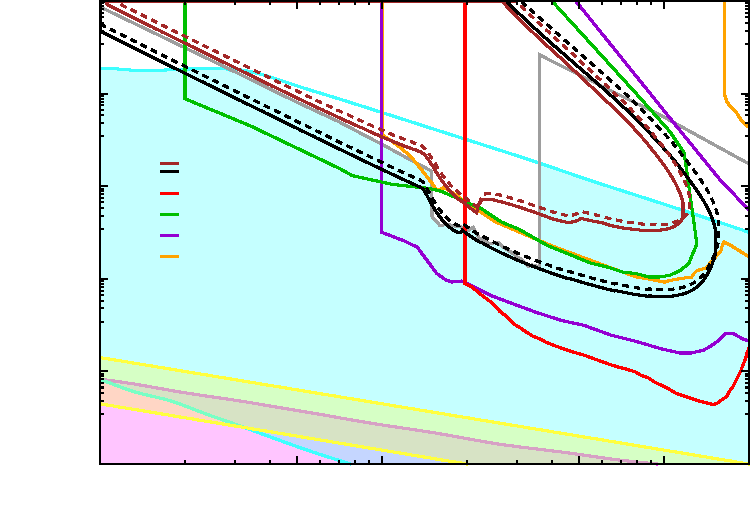
\includegraphics{pics/DUNE_HNL_T_real}}%
    \gplfronttext
  \end{picture}%
\endgroup
}}
	%
	\vspace{-0.2em}
	\caption[Combined sensitivity for dominant mixings for channels with good discovery prospects]%
		{The 90\,\% C.L. sensitivity regions for dominant mixings %
		$|U_{e N}|^2$ (top left), $|U_{\mu N}|^2$ (top right), and $|U_{\tau N}|^2$ (bottom) are presented %
		combining results for channels with good discovery prospects (see text).
		The study is performed for Majorana neutrinos (solid) and Dirac neutrinos (dashed), %
		in the case of no background (black) and after the background analysis (brown).
		The region excluded by experimental constraints (grey) is obtained by combining the results from
		PS191~\cite{Bernardi:1985ny, Bernardi:1987ek}, %
		peak searches~\cite{Artamonov:2014urb, Britton:1992pg, Britton:1992xv, Aguilar-Arevalo:2017vlf, Aguilar-Arevalo:2019owf}, %
		CHARM~\cite{Vilain:1994vg}, NuTeV~\cite{Vaitaitis:1999wq}, DELPHI~\cite{Abreu:1996pa}, and T2K~\cite{Abe:2019kgx}, %
		with the lines reinterpreted for Majorana neutrinos (see \refref{Ruchayskiy:2011aa}).
		The sensitivity for DUNE ND (black) is compared to the predictions of future experiments, %
		SBN~\cite{Ballett:2016opr} (blue), %
		SHiP~\cite{Alekhin:2015byh} (red), NA62~\cite{Drewes:2018irr} (green), MATHUSLA~\cite{Curtin:2018mvb} (purple), %
		and FASER~\cite{Kling:2018wct} with 1\,m radius (orange).
		The shaded areas corresponds to possible neutrino mass models considered in this work: %
		the simulations of the ISS\,(2,2) and ISS\,(2,3) models where the lightest %
		pseudo-Dirac pair is the neutrino decaying in the ND (cyan); %
		the ISS\,(2,3) scenario when the single Majorana state is responsible for a signal (magenta); %
		the type~I seesaw scenario with a neutrino mass starting from \np{20}\,meV to \np{0.2}\,eV (yellow).}
	\label{fig:sensAll}
\end{figure}

A comparison with previous experiments allows to appreciate the ND performance to searches of HNLs.
The results of PS191~\cite{Bernardi:1985ny, Bernardi:1987ek}, peak searches~\cite{Artamonov:2014urb, Britton:1992pg, Britton:1992xv}, %
CHARM~\cite{Vilain:1994vg}, NuTeV~\cite{Vaitaitis:1999wq}, DELPHI~\cite{Abreu:1996pa}, and T2K~\cite{Abe:2019kgx} are also shown %
in \reffig{fig:sensAll}.
It is found that DUNE ND can increase the bound on the electronic and muonic mixing elements %
for masses $m_N < m_{K^0}$ with respect to past experiments.
The constraint on the tauonic mixing is at least comparable with previous measurements.
For masses above, for which neutrino production relies on charm meson decays, the existing bounds %
are improved for the electronic mixing and the tauonic mixing, while a conservative result %
can be achieved in the muonic case.
Also the prospects for the SBN programme~\cite{Ballett:2016opr}, %
NA62~\cite{Drewes:2018irr}, and the proposed SHiP~\cite{Alekhin:2015byh}, MATHUSLA~\cite{Curtin:2018mvb}, %
and FASER~\cite{Kling:2018wct} with 1\,m radius are overlaid.
DUNE ND will give the best sensitivity for masses below the 0.5\,GeV in all channels, but the tauonic one.
However, anywhere the $D_s$ meson production is involved, the experiment cannot outperform the predicted %
sensitivity of the SHiP experiment which will deploy a 400\,GeV proton beam on a titanium-zinc-molybdenum alloy %
target, enhancing the production of charm and bottom mesons.
MATHUSLA will have a similar sensitivity, collecting particles from the High Luminosity LHC phase.
NA62 gives better results for the $|U_{\mu N}|^2$ mixing, but DUNE has a better sensitivity %
to the electron and tau channels.
FASER is comparable to NA62 in sensitivity, but it can reach regions of the parameter space beyond the 2\,GeV limit %
to which DUNE is not sensitive.
Comparing to previous similar studies, the sensitivities estimated in this analysis give stronger %
or at least comparable bounds than the ones in \refref{Krasnov:2019kdc}, 
where a different ND configuration is assumed, and no background study was performed.
More specifically, the limits on $|U_{eN}|^2$ are stronger, even considering the background events.
This is true also for the limits on $|U_{\mu N}|^2$, but only for masses below 500 MeV: %
in \refref{Krasnov:2019kdc} the sensitivity to masses above this threshold is enhanced by the contribution %
from B meson, which is not estimated in this study.
For the same reason, the limits on $|U_{\tau N}|^2$ prove to be comparable to the result of this work, %
despite accounting only for the $D_s$ meson component.

Finally, the overall sensitivity is compared with respect to regions allowed by neutrino mass models.
In the electronic and muonic channels, DUNE ND will be sensitive to a large part of the pseudo-Dirac regions, %
corresponding to ISS\,(2,2) and ISS\,(2,3) models, %
part of which have been already excluded by past experiments.
DUNE will close the gap and put to test type I seesaw parameters, especially for HNL masses between 0.2 and 0.5\,GeV, %
starting to reach the region of ISS\,(2,3) with large lepton number violation.
For the tauonic channel, the experiment will probe only a small portion %
of pseudo-Dirac pairs from ISS\,(2,2) and ISS\,(2,3) models.
The sensitivity is not high enough to reach type I and Majorana state regions, which not even the dedicated experiment SHiP can.

\begin{figure}
	\centering
	{\resizebox{\linewidth}{!}{% GNUPLOT: LaTeX picture with Postscript
\begingroup
  \makeatletter
  \providecommand\color[2][]{%
    \GenericError{(gnuplot) \space\space\space\@spaces}{%
      Package color not loaded in conjunction with
      terminal option `colourtext'%
    }{See the gnuplot documentation for explanation.%
    }{Either use 'blacktext' in gnuplot or load the package
      color.sty in LaTeX.}%
    \renewcommand\color[2][]{}%
  }%
  \providecommand\includegraphics[2][]{%
    \GenericError{(gnuplot) \space\space\space\@spaces}{%
      Package graphicx or graphics not loaded%
    }{See the gnuplot documentation for explanation.%
    }{The gnuplot epslatex terminal needs graphicx.sty or graphics.sty.}%
    \renewcommand\includegraphics[2][]{}%
  }%
  \providecommand\rotatebox[2]{#2}%
  \@ifundefined{ifGPcolor}{%
    \newif\ifGPcolor
    \GPcolortrue
  }{}%
  \@ifundefined{ifGPblacktext}{%
    \newif\ifGPblacktext
    \GPblacktexttrue
  }{}%
  % define a \g@addto@macro without @ in the name:
  \let\gplgaddtomacro\g@addto@macro
  % define empty templates for all commands taking text:
  \gdef\gplbacktext{}%
  \gdef\gplfronttext{}%
  \makeatother
  \ifGPblacktext
    % no textcolor at all
    \def\colorrgb#1{}%
    \def\colorgray#1{}%
  \else
    % gray or color?
    \ifGPcolor
      \def\colorrgb#1{\color[rgb]{#1}}%
      \def\colorgray#1{\color[gray]{#1}}%
      \expandafter\def\csname LTw\endcsname{\color{white}}%
      \expandafter\def\csname LTb\endcsname{\color{black}}%
      \expandafter\def\csname LTa\endcsname{\color{black}}%
      \expandafter\def\csname LT0\endcsname{\color[rgb]{1,0,0}}%
      \expandafter\def\csname LT1\endcsname{\color[rgb]{0,1,0}}%
      \expandafter\def\csname LT2\endcsname{\color[rgb]{0,0,1}}%
      \expandafter\def\csname LT3\endcsname{\color[rgb]{1,0,1}}%
      \expandafter\def\csname LT4\endcsname{\color[rgb]{0,1,1}}%
      \expandafter\def\csname LT5\endcsname{\color[rgb]{1,1,0}}%
      \expandafter\def\csname LT6\endcsname{\color[rgb]{0,0,0}}%
      \expandafter\def\csname LT7\endcsname{\color[rgb]{1,0.3,0}}%
      \expandafter\def\csname LT8\endcsname{\color[rgb]{0.5,0.5,0.5}}%
    \else
      % gray
      \def\colorrgb#1{\color{black}}%
      \def\colorgray#1{\color[gray]{#1}}%
      \expandafter\def\csname LTw\endcsname{\color{white}}%
      \expandafter\def\csname LTb\endcsname{\color{black}}%
      \expandafter\def\csname LTa\endcsname{\color{black}}%
      \expandafter\def\csname LT0\endcsname{\color{black}}%
      \expandafter\def\csname LT1\endcsname{\color{black}}%
      \expandafter\def\csname LT2\endcsname{\color{black}}%
      \expandafter\def\csname LT3\endcsname{\color{black}}%
      \expandafter\def\csname LT4\endcsname{\color{black}}%
      \expandafter\def\csname LT5\endcsname{\color{black}}%
      \expandafter\def\csname LT6\endcsname{\color{black}}%
      \expandafter\def\csname LT7\endcsname{\color{black}}%
      \expandafter\def\csname LT8\endcsname{\color{black}}%
    \fi
  \fi
    \setlength{\unitlength}{0.0500bp}%
    \ifx\gptboxheight\undefined%
      \newlength{\gptboxheight}%
      \newlength{\gptboxwidth}%
      \newsavebox{\gptboxtext}%
    \fi%
    \setlength{\fboxrule}{0.5pt}%
    \setlength{\fboxsep}{1pt}%
\begin{picture}(14400.00,5040.00)%
    \gplgaddtomacro\gplbacktext{%
      \csname LTb\endcsname%%
      \put(444,972){\makebox(0,0)[r]{\strut{}\np{e-1}}}%
      \put(444,2740){\makebox(0,0)[r]{\strut{}\np{e0}}}%
      \put(444,4507){\makebox(0,0)[r]{\strut{}\np{e1}}}%
      \put(576,220){\makebox(0,0){\strut{}\np{e-10}}}%
      \put(1497,220){\makebox(0,0){\strut{}\np{e-8}}}%
      \put(2419,220){\makebox(0,0){\strut{}\np{e-6}}}%
      \put(3340,220){\makebox(0,0){\strut{}\np{e-4}}}%
      \put(4262,220){\makebox(0,0){\strut{}\np{e-2}}}%
    }%
    \gplgaddtomacro\gplfronttext{%
      \csname LTb\endcsname%%
      \put(-304,2739){\rotatebox{-270}{\makebox(0,0){\strut{}$\Delta m_{4 1}^2 $}}}%
      \put(2879,-110){\makebox(0,0){\strut{}$|U_{e 4}|^2$}}%
      \csname LTb\endcsname%%
      \put(1167,4844){\makebox(0,0)[l]{\strut{}DANSS}}%
      \csname LTb\endcsname%%
      \put(1167,4580){\makebox(0,0)[l]{\strut{}NEOS}}%
      \csname LTb\endcsname%%
      \put(1167,4316){\makebox(0,0)[l]{\strut{}STEREO}}%
      \csname LTb\endcsname%%
      \put(1167,4052){\makebox(0,0)[l]{\strut{}SK + IC}}%
    }%
    \gplgaddtomacro\gplbacktext{%
      \csname LTb\endcsname%%
      \put(5052,972){\makebox(0,0)[r]{\strut{}}}%
      \put(5052,2740){\makebox(0,0)[r]{\strut{}}}%
      \put(5052,4507){\makebox(0,0)[r]{\strut{}}}%
      \put(5184,220){\makebox(0,0){\strut{}\np{e-12}}}%
      \put(5952,220){\makebox(0,0){\strut{}\np{e-10}}}%
      \put(6720,220){\makebox(0,0){\strut{}\np{e-8}}}%
      \put(7488,220){\makebox(0,0){\strut{}\np{e-6}}}%
      \put(8255,220){\makebox(0,0){\strut{}\np{e-4}}}%
      \put(9023,220){\makebox(0,0){\strut{}\np{e-2}}}%
    }%
    \gplgaddtomacro\gplfronttext{%
      \csname LTb\endcsname%%
      \put(7487,-110){\makebox(0,0){\strut{}$4 |U_{e 4}|^2 |U_{\mu 4}|^2$}}%
      \csname LTb\endcsname%%
      \put(5775,4844){\makebox(0,0)[l]{\strut{}MiniBooNE}}%
      \csname LTb\endcsname%%
      \put(5775,4580){\makebox(0,0)[l]{\strut{}KARMEN}}%
      \csname LTb\endcsname%%
      \put(5775,4316){\makebox(0,0)[l]{\strut{}OPERA}}%
    }%
    \gplgaddtomacro\gplbacktext{%
      \csname LTb\endcsname%%
      \put(9660,972){\makebox(0,0)[r]{\strut{}}}%
      \put(9660,2740){\makebox(0,0)[r]{\strut{}}}%
      \put(9660,4507){\makebox(0,0)[r]{\strut{}}}%
      \put(14399,220){\makebox(0,0){\strut{}\np{e0}}}%
      \put(9792,220){\makebox(0,0){\strut{}\np{e-10}}}%
      \put(10713,220){\makebox(0,0){\strut{}\np{e-8}}}%
      \put(11635,220){\makebox(0,0){\strut{}\np{e-6}}}%
      \put(12556,220){\makebox(0,0){\strut{}\np{e-4}}}%
      \put(13478,220){\makebox(0,0){\strut{}\np{e-2}}}%
    }%
    \gplgaddtomacro\gplfronttext{%
      \csname LTb\endcsname%%
      \put(12095,-110){\makebox(0,0){\strut{}$|U_{\mu 4}|^2$}}%
      \csname LTb\endcsname%%
      \put(10383,4844){\makebox(0,0)[l]{\strut{}$\nu_\mu\to\nu_\mu$}}%
    }%
    \gplbacktext
    \put(0,0){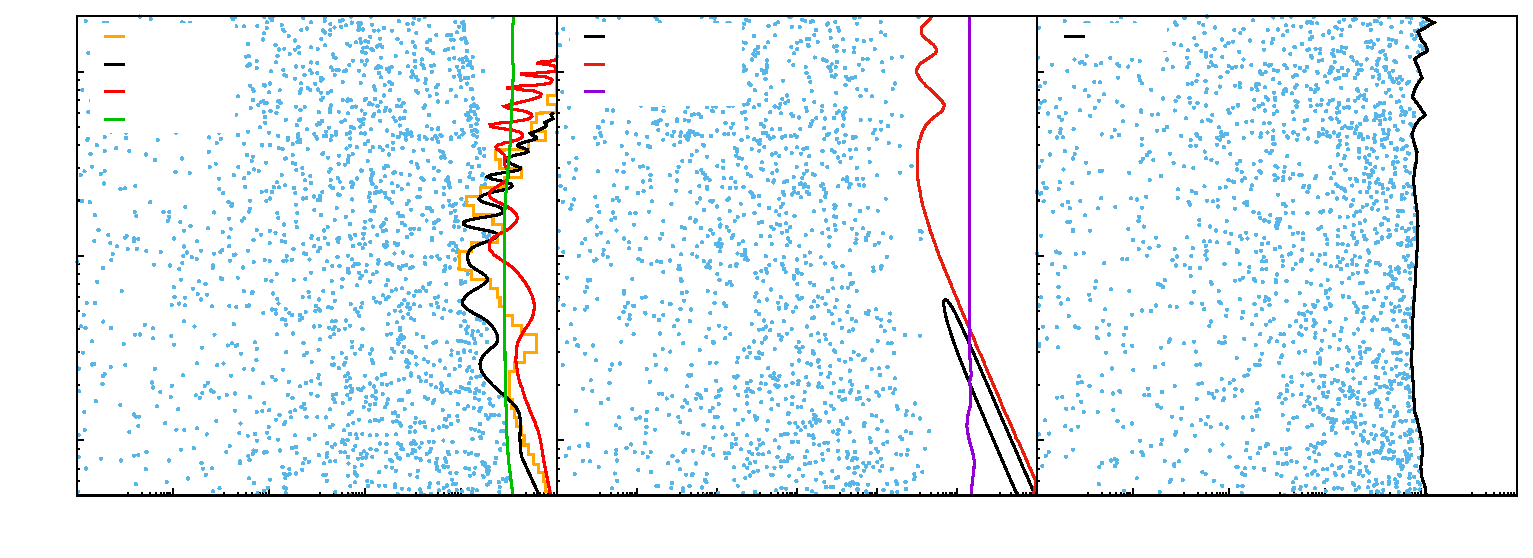
\includegraphics{pics/multiSBL}}%
    \gplfronttext
  \end{picture}%
\endgroup
}}
	%{\resizebox{0.5\linewidth}{!}{\input{pics/oscUe.tex}}}
	%\hspace{-1em}
	%{\resizebox{0.5\linewidth}{!}{\input{pics/oscUem.tex}}}
	%\hspace{-1em}
	%{\resizebox{0.5\linewidth}{!}{\input{pics/oscUm.tex}}}
	%
	\caption[Comparison of ISS(2,3) with short baseline anomalies]%
		{One of the two ISS\,(2,3) realisations considered presents a Majorana state at masses comparable with short baseline experiments.
		The results of the ISS\,(2,3) simulation (blue dots) for $\Delta m_{4 1}^2$ against combination of mixing angles and %
		the experimental result at 90\,\% C.L. are shown.
		$|U_{e 4}|^2$~(left) compared to %
		to DANSS~\cite{Alekseev:2018efk}, NEOS~\cite{Ko:2016owz}, STEREO~\cite{AlmazanMolina:2019qul}, %
		and Super-Kamiokande and IceCube combined ~\cite{Dentler:2018sju};
		\mbox{$\sin^2 2\theta{_\mu e} = 4|U_{e 4}|^2|U_{\mu 4}|^2$} (middle) compared to KARMEN2, OPERA and MiniBooNE~\cite{Aguilar-Arevalo:2018gpe},
		and $|U_{\mu 4}|^2$ (right) compared to a combined $\nu_\mu$ disappearance analysis~\cite{Dentler:2018sju}.
		Only the points generated by matrices which pass the experimental constraints are shown here.}
	\label{fig:sblosc}
\end{figure}

The ISS\,(2,3) scenario in which the pseudo-Dirac pair is accessible by the experiment also predicts a light %
Majorana state, the mass of which is controlled by the small LNV perturbations.
This entails the presence of a third mass splitting $\Delta m^2_{4 1}$, which could give %
an active--sterile oscillation signature in short baseline experiments, very much debated in literature %
(see \refref{Dentler:2018sju} for a recent review).
In figure Fig.~\ref{fig:sblosc}, the new mass splitting is plotted against the mixings $|U_{e 4}|^2$, %
$|U_{\mu 4}|^2$ and the combination usually referred to as %
$\sin^2 2\theta_{\mu e} \equiv 4 |U_{e 4}|^2|U_{\mu 4}|^2$.
The mass splittings generated in the matrix scan span from %
$\Delta m^2_{3 1} \simeq \np{0.0025}$\,eV\tapi{2} up to \np{e4}\,eV\tapi{2}, and the squared mixings cover a large region, %
down to \np{e-14} for all the flavours.
The reactor anomalies could be soon excluded at the 90\,\% C.L. by the DANSS experiment~\cite{Alekseev:2018efk} %
and the allowed regions from LSND~\cite{Aguilar:2001ty} and %
MiniBooNE~\cite{Aguilar-Arevalo:2012fmn, Aguilar-Arevalo:2013pmq, Aguilar-Arevalo:2018gpe} %
require values of $\sin^2 2\theta_{\mu e} \gtrsim \np{e-3}$.
The regions already excluded by these experiments are also reported in \reffig{fig:sblosc}.
Given the results of the matrix scan, it is unlikely that one of the ISS\,(2,3) realisations %
considered in this work could explain simultaneously a short baseline anomaly and predict %
a heavy neutrino--like signal in DUNE ND, unless for sparse and very fine-tuned points.


\section{Determining the nature of HNLs}
\label{sec:majorana_dirac}


If such heavy neutrino states are discovered, it would be possible to distinguish the fermionic nature %
of the decaying HNL, by studying the charge of the decay products.
Thanks to the different angular dependency of polarised decay rates for Majorana and Dirac, analysing the angular distributions of %
HNL decays could be in principle used to distinguish between the two scenarios~\cite{Balantekin:2018ukw}.
As studied in~\refsec{sec:decay}, the two-body decay distributions for a Majorana neutrino %
with given helicity into a neutral final state is isotropic in the heavy neutrino rest frame.
This is also true of the total decay distribution of charged final states in the absence of charge-ID in the detector.
For two-body semileptonic decays, the polarised decay rate has a linear or antilinear dependency on $\cos\theta$ in the rest frame, %
according to the polarisation and lepton number of the neutrino, where $\theta$ is the polar angle of the charged lepton to the beamline.
However, for practical applications, studying angular distributions requires modest statistics %
and such distributions might not be obvious anymore once they are convolved with the neutrino spectrum.
%This could in principle be used to determine the nature of the heavy neutrino.

It is worth noting, that aside from the neutral current distributional differences, %
the direct distinction between charged-conjugate final states is an equally competitive means of determining the nature of the initial state.
The discussion of this section focuses on the channels $N \to \ell^\mp P^\pm$, %
as these present the best discovery prospect.
The decays into charged pseudoscalar mesons $P^\pm$ are the channel with the highest branching ratio (see \refsec{sec:decay}) %
and the ones with the cleanest experimental signature, despite the nonnegligible background.
Moreover, the charge of the final state lepton is directly determined by the fermionic type of the decaying neutrino.
Assuming a beam purely composed of neutrinos, a Dirac HNL produced in the beam could only decay into $\ell^- P^+$, %
as it preserves lepton number.
On the other hand, if the heavy neutrino is Majorana, the LNV channel $\ell^+ P^-$ %
would be also expected with the same rate as the LNC mode.
With perfect detector efficiency and performance, only one LNV event is necessary to reject LNC.
In addition to the different event rate, the angular and energy distribution of the decays will vary %
depending on the fermionic nature of the neutrino, because of different helicity contributions.
However, a beam of only neutrino is not achievable with %
the conventional techniques for producing artificial neutrinos.
Unsuccessful focusing and deflection by the horn system for short-lived secondary particles is the cause %
of an irremovable component of antineutrinos in the neutrino mode beam. %, and vice versa for the antineutrino mode.
This results in an intrinsic background of LNV events, which are not expected in the case of a Dirac neutrino.
The same discussion applies equally to the beam in antineutrino mode.

%We assume the beam to be in FHC mode only and we focus only on the channel $N\to \ell \pi$.
%If there is no contamination from $\cj{\nu}$, then beam is purely $\nu$.
%This means that after mixing with HNL, in the Dirac case the decay can only happen in the channel $N\to \ell^- \pi^+$.
%If the HNL is Majorana, we would see equal number of decays into $N \to \ell^\mp \pi^\pm$.

Neglecting background from SM events, the number of HNL decay events inside the detector is computed %
using \refeq{eq:event}.
%The number of events is computed for each point of the parameter space.
%For each point of the parameter space $\hat{\theta} = (m_N, |U_{\alpha N}|^2)$, we can predict the number %
%of events detected at ND for both channels $\ell^- \pi^+$ and $\ell^+ \pi^-$.
For given HNL mass and mixings, let us define $\sigma$ and $\rho$ respectively as %
the number of signal events for the channel $\ell^- \pi^+$ and for the channel $\ell^+ \pi^-$.
The probability of detecting $s$ and $r$ events in the detector for the two channels %
follows a Poisson distribution with rate parameter respectively $\sigma$ and $\rho$:
\begin{equation}
	%P(n^{m,p}; \hat{\theta}) = P(n^m, \sigma^m)\,P(n^p, \sigma^p) = 
	P(s, r) = e^{-\sigma} \frac{\sigma^s}{s!}\ e^{-\rho} \frac{\rho^r}{r!}\ .
\end{equation}
With this probability definition, a frequentist confidence regions is defined %
for each given point of the parameter space, i.e. a combination of $\sigma$ and $\rho$, %
sorting by the ratio of probabilities~\cite{Feldman:1997qc} %
\begin{equation}
	\frac{P(s, r)}{P(\hat{s}, \hat{r})}\ ,
\end{equation}
where the best fit points are $\hat{s} = \sigma$ and $\hat{r} = \rho$ if the HNL is Dirac %
or $\hat{s} = \hat{r} = (\sigma + \rho)/2$ if Majorana.
The Poissonian probabilities are then summed until reaching 99\,\%\ C.L., %
determining in this way a region in the $(\sigma, \rho)$ space.
If the two regions for the case of Dirac or Majorana HNL do not overlap, %
then it is possible to distinguish between the two scenarios with 99\,\%\ C.L.
SM background can be accounted for by replacing $\sigma \to \sigma + b_\sigma$ and $\rho \to \rho + b_\rho$.

%Neglecting background induced by SM interactions of light neutrinos with the detector, the number of channel $d$ decays inside the detector is estimated as:
%\begin{equation}
%	\label{eq:event}
%	\mathcal{N}_d = \int\!\! \dd{E}\ \Pi_d(E) \, \dv{\phi_N}{E}\ ,
%\end{equation}
%where $\dv*{\phi_N}{E}$ is the flux of HNL expected at the ND, and $\Pi_d(E)$ encapsulates the probability of an HNL of energy $E$ to travel the baseline %
%distance and decay inside the ND to the specific channel $d$.
%The number of events is computed for each point of the parameter space.
%In this region, the horn system is the most effective in deflecting pions and kaons, %
%achieving a reduction factor of 10 for the antineutrino subcomponent.
%Using the Feldman and Cousins method~\cite{Feldman:1997qc}, we estimate how many events are needed in order %
%The probability of observing $n$ events with a signal mean $\sigma = \mathcal{N}_d$ %
%and background $b = \mathcal{B}_d$ follows a Poisson distribution:
%\begin{equation*}
%	P(n|\sigma,b) = (\sigma+b) \frac{e^{-(\sigma+b)}}{n!}
%\end{equation*}
%
%The null hypothesis is that no LNV is seen, just LNC events.
%The signal must be above the intrinsic background of the antineutrino subcomponent.
%So for a given point in the parameter space, $b$ is the number of events in the ``negative'' channel %
%by Dirac decays (so antineutrinos are decaying), $s$ required is the one of good LNV signals, %
%which is Majorana decays to the LNV channel.
%
%The number of events for each point of the parameter space is computed 
%The null hypothesis $H_0$ is that no sterile neutrino decays are seen ($\sigma = 0$), %
%while only background events $b$ are expected.
%The Feldman and Cousins method~\cite{Feldman:1997qc} is the applied to reject the null hypothesis that no LNV event is seen.
%This criterion is used to define the sensitivity regions to LNV event by HNL decay, shown later.

\begin{figure}[t]
	\centering
	\resizebox{.48\textwidth}{!}{% GNUPLOT: LaTeX picture with Postscript
\begingroup
  \makeatletter
  \providecommand\color[2][]{%
    \GenericError{(gnuplot) \space\space\space\@spaces}{%
      Package color not loaded in conjunction with
      terminal option `colourtext'%
    }{See the gnuplot documentation for explanation.%
    }{Either use 'blacktext' in gnuplot or load the package
      color.sty in LaTeX.}%
    \renewcommand\color[2][]{}%
  }%
  \providecommand\includegraphics[2][]{%
    \GenericError{(gnuplot) \space\space\space\@spaces}{%
      Package graphicx or graphics not loaded%
    }{See the gnuplot documentation for explanation.%
    }{The gnuplot epslatex terminal needs graphicx.sty or graphics.sty.}%
    \renewcommand\includegraphics[2][]{}%
  }%
  \providecommand\rotatebox[2]{#2}%
  \@ifundefined{ifGPcolor}{%
    \newif\ifGPcolor
    \GPcolortrue
  }{}%
  \@ifundefined{ifGPblacktext}{%
    \newif\ifGPblacktext
    \GPblacktexttrue
  }{}%
  % define a \g@addto@macro without @ in the name:
  \let\gplgaddtomacro\g@addto@macro
  % define empty templates for all commands taking text:
  \gdef\gplbacktext{}%
  \gdef\gplfronttext{}%
  \makeatother
  \ifGPblacktext
    % no textcolor at all
    \def\colorrgb#1{}%
    \def\colorgray#1{}%
  \else
    % gray or color?
    \ifGPcolor
      \def\colorrgb#1{\color[rgb]{#1}}%
      \def\colorgray#1{\color[gray]{#1}}%
      \expandafter\def\csname LTw\endcsname{\color{white}}%
      \expandafter\def\csname LTb\endcsname{\color{black}}%
      \expandafter\def\csname LTa\endcsname{\color{black}}%
      \expandafter\def\csname LT0\endcsname{\color[rgb]{1,0,0}}%
      \expandafter\def\csname LT1\endcsname{\color[rgb]{0,1,0}}%
      \expandafter\def\csname LT2\endcsname{\color[rgb]{0,0,1}}%
      \expandafter\def\csname LT3\endcsname{\color[rgb]{1,0,1}}%
      \expandafter\def\csname LT4\endcsname{\color[rgb]{0,1,1}}%
      \expandafter\def\csname LT5\endcsname{\color[rgb]{1,1,0}}%
      \expandafter\def\csname LT6\endcsname{\color[rgb]{0,0,0}}%
      \expandafter\def\csname LT7\endcsname{\color[rgb]{1,0.3,0}}%
      \expandafter\def\csname LT8\endcsname{\color[rgb]{0.5,0.5,0.5}}%
    \else
      % gray
      \def\colorrgb#1{\color{black}}%
      \def\colorgray#1{\color[gray]{#1}}%
      \expandafter\def\csname LTw\endcsname{\color{white}}%
      \expandafter\def\csname LTb\endcsname{\color{black}}%
      \expandafter\def\csname LTa\endcsname{\color{black}}%
      \expandafter\def\csname LT0\endcsname{\color{black}}%
      \expandafter\def\csname LT1\endcsname{\color{black}}%
      \expandafter\def\csname LT2\endcsname{\color{black}}%
      \expandafter\def\csname LT3\endcsname{\color{black}}%
      \expandafter\def\csname LT4\endcsname{\color{black}}%
      \expandafter\def\csname LT5\endcsname{\color{black}}%
      \expandafter\def\csname LT6\endcsname{\color{black}}%
      \expandafter\def\csname LT7\endcsname{\color{black}}%
      \expandafter\def\csname LT8\endcsname{\color{black}}%
    \fi
  \fi
    \setlength{\unitlength}{0.0500bp}%
    \ifx\gptboxheight\undefined%
      \newlength{\gptboxheight}%
      \newlength{\gptboxwidth}%
      \newsavebox{\gptboxtext}%
    \fi%
    \setlength{\fboxrule}{0.5pt}%
    \setlength{\fboxsep}{1pt}%
\begin{picture}(7200.00,5040.00)%
    \gplgaddtomacro\gplbacktext{%
      \csname LTb\endcsname%%
      \put(747,595){\makebox(0,0)[r]{\strut{}\np{e-12}}}%
      \csname LTb\endcsname%%
      \put(747,1484){\makebox(0,0)[r]{\strut{}\np{e-10}}}%
      \csname LTb\endcsname%%
      \put(747,2373){\makebox(0,0)[r]{\strut{}\np{e-8}}}%
      \csname LTb\endcsname%%
      \put(747,3261){\makebox(0,0)[r]{\strut{}\np{e-6}}}%
      \csname LTb\endcsname%%
      \put(747,4150){\makebox(0,0)[r]{\strut{}\np{e-4}}}%
      \csname LTb\endcsname%%
      \put(747,5039){\makebox(0,0)[r]{\strut{}\np{e-2}}}%
      \csname LTb\endcsname%%
      \put(2773,409){\makebox(0,0){\strut{}0.05}}%
      \csname LTb\endcsname%%
      \put(5526,409){\makebox(0,0){\strut{}0.5}}%
      \csname LTb\endcsname%%
      \put(7183,409){\makebox(0,0){\strut{}2}}%
      \csname LTb\endcsname%%
      \put(849,409){\makebox(0,0){\strut{}0.01}}%
      \csname LTb\endcsname%%
      \put(3602,409){\makebox(0,0){\strut{}0.1}}%
      \csname LTb\endcsname%%
      \put(6354,409){\makebox(0,0){\strut{}1}}%
    }%
    \gplgaddtomacro\gplfronttext{%
      \csname LTb\endcsname%%
      \put(153,2817){\rotatebox{-270}{\makebox(0,0){\strut{}$|U_{e N}|^2$}}}%
      \csname LTb\endcsname%%
      \put(4016,130){\makebox(0,0){\strut{}Mass (GeV)}}%
      \csname LTb\endcsname%%
      \put(4466,3543){\makebox(0,0)[l]{\strut{}FASER}}%
      \csname LTb\endcsname%%
      \put(4466,3747){\makebox(0,0)[l]{\strut{}NA62}}%
      \csname LTb\endcsname%%
      \put(4466,3951){\makebox(0,0)[l]{\strut{}SHiP}}%
      \csname LTb\endcsname%%
      \put(4466,4155){\makebox(0,0)[l]{\strut{}SBND}}%
      \csname LTb\endcsname%%
      \put(4466,4359){\makebox(0,0)[l]{\strut{}DUNE}}%
      \csname LTb\endcsname%%
      \put(747,595){\makebox(0,0)[r]{\strut{}\np{e-12}}}%
      \csname LTb\endcsname%%
      \put(747,1484){\makebox(0,0)[r]{\strut{}\np{e-10}}}%
      \csname LTb\endcsname%%
      \put(747,2373){\makebox(0,0)[r]{\strut{}\np{e-8}}}%
      \csname LTb\endcsname%%
      \put(747,3261){\makebox(0,0)[r]{\strut{}\np{e-6}}}%
      \csname LTb\endcsname%%
      \put(747,4150){\makebox(0,0)[r]{\strut{}\np{e-4}}}%
      \csname LTb\endcsname%%
      \put(747,5039){\makebox(0,0)[r]{\strut{}\np{e-2}}}%
      \csname LTb\endcsname%%
      \put(2773,409){\makebox(0,0){\strut{}0.05}}%
      \csname LTb\endcsname%%
      \put(5526,409){\makebox(0,0){\strut{}0.5}}%
      \csname LTb\endcsname%%
      \put(7183,409){\makebox(0,0){\strut{}2}}%
      \csname LTb\endcsname%%
      \put(849,409){\makebox(0,0){\strut{}0.01}}%
      \csname LTb\endcsname%%
      \put(3602,409){\makebox(0,0){\strut{}0.1}}%
      \csname LTb\endcsname%%
      \put(6354,409){\makebox(0,0){\strut{}1}}%
      \csname LTb\endcsname%%
      \put(2073,4050){\makebox(0,0)[l]{\strut{}\textbf{Excluded}}}%
      \csname LTb\endcsname%%
      \put(1678,1039){\makebox(0,0)[l]{\strut{}\textbf{Majorana state}}}%
      \csname LTb\endcsname%%
      \put(5554,906){\makebox(0,0)[l]{\strut{}\textbf{\shortstack{Pseudo-Dirac\\pair}}}}%
      \csname LTb\endcsname%%
      \put(2773,1928){\rotatebox{-5}{\makebox(0,0)[l]{\strut{}\textbf{Type I}}}}%
    }%
    \gplbacktext
    \put(0,0){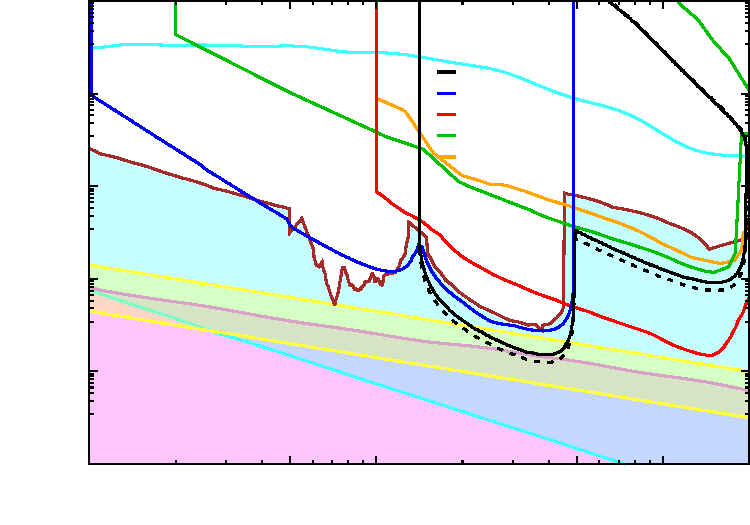
\includegraphics{pics/lnvexp_E}}%
    \gplfronttext
  \end{picture}%
\endgroup
}
	\resizebox{.48\textwidth}{!}{% GNUPLOT: LaTeX picture with Postscript
\begingroup
  \makeatletter
  \providecommand\color[2][]{%
    \GenericError{(gnuplot) \space\space\space\@spaces}{%
      Package color not loaded in conjunction with
      terminal option `colourtext'%
    }{See the gnuplot documentation for explanation.%
    }{Either use 'blacktext' in gnuplot or load the package
      color.sty in LaTeX.}%
    \renewcommand\color[2][]{}%
  }%
  \providecommand\includegraphics[2][]{%
    \GenericError{(gnuplot) \space\space\space\@spaces}{%
      Package graphicx or graphics not loaded%
    }{See the gnuplot documentation for explanation.%
    }{The gnuplot epslatex terminal needs graphicx.sty or graphics.sty.}%
    \renewcommand\includegraphics[2][]{}%
  }%
  \providecommand\rotatebox[2]{#2}%
  \@ifundefined{ifGPcolor}{%
    \newif\ifGPcolor
    \GPcolortrue
  }{}%
  \@ifundefined{ifGPblacktext}{%
    \newif\ifGPblacktext
    \GPblacktexttrue
  }{}%
  % define a \g@addto@macro without @ in the name:
  \let\gplgaddtomacro\g@addto@macro
  % define empty templates for all commands taking text:
  \gdef\gplbacktext{}%
  \gdef\gplfronttext{}%
  \makeatother
  \ifGPblacktext
    % no textcolor at all
    \def\colorrgb#1{}%
    \def\colorgray#1{}%
  \else
    % gray or color?
    \ifGPcolor
      \def\colorrgb#1{\color[rgb]{#1}}%
      \def\colorgray#1{\color[gray]{#1}}%
      \expandafter\def\csname LTw\endcsname{\color{white}}%
      \expandafter\def\csname LTb\endcsname{\color{black}}%
      \expandafter\def\csname LTa\endcsname{\color{black}}%
      \expandafter\def\csname LT0\endcsname{\color[rgb]{1,0,0}}%
      \expandafter\def\csname LT1\endcsname{\color[rgb]{0,1,0}}%
      \expandafter\def\csname LT2\endcsname{\color[rgb]{0,0,1}}%
      \expandafter\def\csname LT3\endcsname{\color[rgb]{1,0,1}}%
      \expandafter\def\csname LT4\endcsname{\color[rgb]{0,1,1}}%
      \expandafter\def\csname LT5\endcsname{\color[rgb]{1,1,0}}%
      \expandafter\def\csname LT6\endcsname{\color[rgb]{0,0,0}}%
      \expandafter\def\csname LT7\endcsname{\color[rgb]{1,0.3,0}}%
      \expandafter\def\csname LT8\endcsname{\color[rgb]{0.5,0.5,0.5}}%
    \else
      % gray
      \def\colorrgb#1{\color{black}}%
      \def\colorgray#1{\color[gray]{#1}}%
      \expandafter\def\csname LTw\endcsname{\color{white}}%
      \expandafter\def\csname LTb\endcsname{\color{black}}%
      \expandafter\def\csname LTa\endcsname{\color{black}}%
      \expandafter\def\csname LT0\endcsname{\color{black}}%
      \expandafter\def\csname LT1\endcsname{\color{black}}%
      \expandafter\def\csname LT2\endcsname{\color{black}}%
      \expandafter\def\csname LT3\endcsname{\color{black}}%
      \expandafter\def\csname LT4\endcsname{\color{black}}%
      \expandafter\def\csname LT5\endcsname{\color{black}}%
      \expandafter\def\csname LT6\endcsname{\color{black}}%
      \expandafter\def\csname LT7\endcsname{\color{black}}%
      \expandafter\def\csname LT8\endcsname{\color{black}}%
    \fi
  \fi
    \setlength{\unitlength}{0.0500bp}%
    \ifx\gptboxheight\undefined%
      \newlength{\gptboxheight}%
      \newlength{\gptboxwidth}%
      \newsavebox{\gptboxtext}%
    \fi%
    \setlength{\fboxrule}{0.5pt}%
    \setlength{\fboxsep}{1pt}%
\begin{picture}(7200.00,5040.00)%
    \gplgaddtomacro\gplbacktext{%
      \csname LTb\endcsname%%
      \put(747,595){\makebox(0,0)[r]{\strut{}\np{e-12}}}%
      \csname LTb\endcsname%%
      \put(747,1484){\makebox(0,0)[r]{\strut{}\np{e-10}}}%
      \csname LTb\endcsname%%
      \put(747,2373){\makebox(0,0)[r]{\strut{}\np{e-8}}}%
      \csname LTb\endcsname%%
      \put(747,3261){\makebox(0,0)[r]{\strut{}\np{e-6}}}%
      \csname LTb\endcsname%%
      \put(747,4150){\makebox(0,0)[r]{\strut{}\np{e-4}}}%
      \csname LTb\endcsname%%
      \put(747,5039){\makebox(0,0)[r]{\strut{}\np{e-2}}}%
      \csname LTb\endcsname%%
      \put(2773,409){\makebox(0,0){\strut{}0.05}}%
      \csname LTb\endcsname%%
      \put(5526,409){\makebox(0,0){\strut{}0.5}}%
      \csname LTb\endcsname%%
      \put(7183,409){\makebox(0,0){\strut{}2}}%
      \csname LTb\endcsname%%
      \put(849,409){\makebox(0,0){\strut{}0.01}}%
      \csname LTb\endcsname%%
      \put(3602,409){\makebox(0,0){\strut{}0.1}}%
      \csname LTb\endcsname%%
      \put(6354,409){\makebox(0,0){\strut{}1}}%
    }%
    \gplgaddtomacro\gplfronttext{%
      \csname LTb\endcsname%%
      \put(153,2817){\rotatebox{-270}{\makebox(0,0){\strut{}$|U_{\mu N}|^2$}}}%
      \csname LTb\endcsname%%
      \put(4016,130){\makebox(0,0){\strut{}Mass $m_N$ (GeV)}}%
      \csname LTb\endcsname%%
      \put(4466,3677){\makebox(0,0)[l]{\strut{}FASER}}%
      \csname LTb\endcsname%%
      \put(4466,3881){\makebox(0,0)[l]{\strut{}NA62}}%
      \csname LTb\endcsname%%
      \put(4466,4085){\makebox(0,0)[l]{\strut{}SHiP}}%
      \csname LTb\endcsname%%
      \put(4466,4289){\makebox(0,0)[l]{\strut{}SBND}}%
      \csname LTb\endcsname%%
      \put(4466,4493){\makebox(0,0)[l]{\strut{}DUNE}}%
      \csname LTb\endcsname%%
      \put(747,595){\makebox(0,0)[r]{\strut{}\np{e-12}}}%
      \csname LTb\endcsname%%
      \put(747,1484){\makebox(0,0)[r]{\strut{}\np{e-10}}}%
      \csname LTb\endcsname%%
      \put(747,2373){\makebox(0,0)[r]{\strut{}\np{e-8}}}%
      \csname LTb\endcsname%%
      \put(747,3261){\makebox(0,0)[r]{\strut{}\np{e-6}}}%
      \csname LTb\endcsname%%
      \put(747,4150){\makebox(0,0)[r]{\strut{}\np{e-4}}}%
      \csname LTb\endcsname%%
      \put(747,5039){\makebox(0,0)[r]{\strut{}\np{e-2}}}%
      \csname LTb\endcsname%%
      \put(2773,409){\makebox(0,0){\strut{}0.05}}%
      \csname LTb\endcsname%%
      \put(5526,409){\makebox(0,0){\strut{}0.5}}%
      \csname LTb\endcsname%%
      \put(7183,409){\makebox(0,0){\strut{}2}}%
      \csname LTb\endcsname%%
      \put(849,409){\makebox(0,0){\strut{}0.01}}%
      \csname LTb\endcsname%%
      \put(3602,409){\makebox(0,0){\strut{}0.1}}%
      \csname LTb\endcsname%%
      \put(6354,409){\makebox(0,0){\strut{}1}}%
      \csname LTb\endcsname%%
      \put(5526,3706){\makebox(0,0)[l]{\strut{}\textbf{Excluded}}}%
      \csname LTb\endcsname%%
      \put(1678,1039){\makebox(0,0)[l]{\strut{}\textbf{Majorana state}}}%
      \csname LTb\endcsname%%
      \put(5554,906){\makebox(0,0)[l]{\strut{}\textbf{\shortstack{Pseudo-Dirac\\pair}}}}%
      \csname LTb\endcsname%%
      \put(2773,1928){\rotatebox{-5}{\makebox(0,0)[l]{\strut{}\textbf{Type I}}}}%
    }%
    \gplbacktext
    \put(0,0){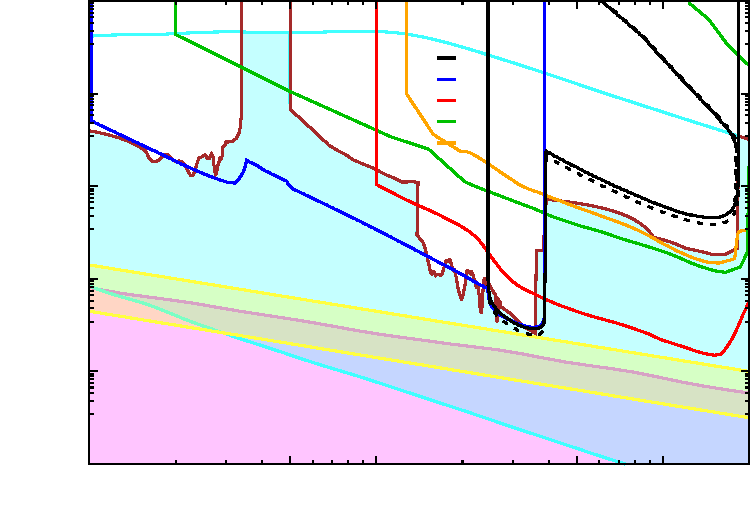
\includegraphics{pics/lnvexp_M}}%
    \gplfronttext
  \end{picture}%
\endgroup
}
	\caption[Sensitivity to distinction between Majorana and Dirac HNL]%
		{The regions in which distinction between Majorana and Dirac HNL is %
		possible with 90\,\% C.L. are shown for dominant $|U_{e N}|^2$ (left) and $|U_{\mu N}|^2$ (right).
		The channels $N \to e^\mp \pi^\pm$ and $\mu^\mp \pi^\pm$ are used, respectively.
		The dashed line black line assumes 100\,\% charge identification, %
		whereas the solid ones correspond to a realistic charge detection efficiency evaluated %
		with a MC simulation.
		The regions are compared to the exclusion limits to HNL discovery of future experiments: %
		SBN~\cite{Ballett:2016opr} (blue), SHiP~\cite{Alekhin:2015byh} (red), %
		NA62~\cite{Drewes:2018irr} (green), MATHUSLA~\cite{Curtin:2018mvb} (purple), %
		and FASER~\cite{Kling:2018wct} with 1\,m radius (orange).
		The region excluded by experimental constraints (brown) is obtained by combining the results from
		PS191~\cite{Bernardi:1985ny, Bernardi:1987ek}, %
		peak searches~\cite{Artamonov:2014urb, Britton:1992pg, Britton:1992xv, Aguilar-Arevalo:2017vlf, Aguilar-Arevalo:2019owf}, %
		CHARM~\cite{Vilain:1994vg}, NuTeV~\cite{Vaitaitis:1999wq}, DELPHI~\cite{Abreu:1996pa}, and T2K~\cite{Abe:2019kgx}.
		The shaded areas corresponds to possible neutrino mass models considered in this work: %
		the simulations of the ISS\,(2,2) and ISS\,(2,3) models where the lightest %
		pseudo-Dirac pair is the neutrino decaying in the ND (cyan); %
		the ISS\,(2,3) scenario when the single Majorana state is responsible for a signal (magenta); %
		the type~I seesaw scenario with a neutrino mass starting from \np{20}\,meV to \np{0.2}\,eV (yellow).}
	\label{fig:lnv}
\end{figure}

Correct charge identification is a necessary requirement to distinguish between %
lepton number conserving and lepton number violating processes.
Being magnetised, the MPD is capable of charge identification of tracks.
An analysis on the determination of the HNL nature by the MPD was carried out in \refref{Berryman:2019dme}.
Although charge identification is a difficult task with liquid argon technology, %
some events originating inside the LArTPC module can propagate to the MPD and the charge of these particles could be identified.
This would allow the expansion of the fiducial volume of the ND sensitive to charges, which depends on the momentum of the final state particles.
Using the same fast MC simulation of the DUNE ND explained in \refsec{sec:experiment}, %
the charge is retrieved if the sagitta of curved tracks inside the MPD are greater than 1\,cm, %
hundred times the spatial resolution.
Assuming a high momentum and neglecting energy loss in the MPD, the condition required is 
\begin{equation}
	%s = R \qty( 1 - \cos \frac{L}{R} ) 
	s \simeq \frac{L^2}{R} \simeq \frac{0.3\,B}{p} L^2 %
	(\cos^2\theta + \sin^2\theta\, \sin^2\phi)^2 > 0.1\,\text{cm}\ ,
\end{equation}
where $B = 0.5$\,T is the magnetic field of the MPD, $p$ the charged particle momentum, %
$L$ the length of the track, and $\theta$ and $\phi$ the polar and azimuth angles.
The 90\,\% C.L. regions in which statistics is sufficient for distinguishing between Majorana and Dirac neutrinos %
are shown in \reffig{fig:lnv}.
As specified above, the two-body pseudoscalar meson channels are used in conjunction with an expanded fiducial volume %
compared to \refref{Berryman:2019dme}.
A background evaluation for this specific analysis is under study.
Charge identification can further reduce background from SM neutrino interactions, %
especially if with production of extra pions and other hadrons.
HNL decays have always particles of opposite charge in the final state and this requirement %
can help reject more background events in the selection process.
